\documentclass[a4paper]{article}

\usepackage[portuguese]{babel}
\usepackage[utf8]{inputenc}
\usepackage[T1]{fontenc}

\newcommand{\documentTitle}{Genetic Algorithms - Brachistochrone Curve} %Macro definition
\newcommand{\documentAuthors}{João Rafael (2008111876, jprafael@student.dei.uc.pt) \and José Ribeiro (2008112181, jbaia@student.dei.uc.pt)} %Macro definition

\title{\documentTitle}
\author{\documentAuthors{}}

\usepackage{hyperref}
\hypersetup{
	pdftitle = \documentTitle
	,pdfauthor = \documentAuthors
	,pdfsubject = {Introduction to Artificial Inteligence Project \#2 Report}
	,pdfkeywords = {Artificial Inteligence Project} {Genetic Algorithms} {Brachistochrone Curve}
	,pdfborder = {0 0 0}
}

\usepackage{subfig}
\usepackage{amsmath}
\usepackage{wrapfig}
\usepackage{array}
\usepackage{anysize}
\usepackage{lscape}
\usepackage[pdftex]{graphicx}
\usepackage{longtable}
\usepackage{multirow}
\usepackage[table]{xcolor}

\marginsize{3.5cm}{3.5cm}{3cm}{3cm}

\makeatletter

\begin{document}
\renewcommand{\figurename}{Figure}
\maketitle
\cleardoublepage

\tableofcontents
\cleardoublepage

\setlength{\parindent}{1cm}
\setlength{\parskip}{0.3cm}

\section{Introduction}
\indent \indent Este projecto está inserido no âmbito da disciplina de Introdução à Inteligência Artificial,
mais concretamente no seguimento do primeiro projecto, uma vez que implementamos outro tipo de Agentes: Agentes Adaptativos.

Ao contrário dos agentes já estudados (Reactivos), estes baseiam-se fundamentalmente em conceitos da Biologia, nomeadamente a teoria da Selecção Natural de Darwin aplicada à Genética.
Estes agentes representam populações que, ao longo do tempo (iterações da aplicação), evoluem ao sofrer mutações e recombinações entre indivíduos (e os seus genes) e posterior selecção dos mais aptos.
Desta forma, pretende-se que a aptidão da população melhore, convergindo para o óptimo global.

\subsection{Brachistochrone curve}

\indent \indent O problema da curva braquistócrona é um clássico da disciplina de cálculo:

\emph{Tendo dois pontos distintos, A e B, o objectivo é conhecer a trajectória que minimiza o tempo que um ponto material demora a deslocar-se entre eles, quando sujeito apenas à força da gravidade (com atrito desprezável).}

\begin{figure}[ht]
	\centering
	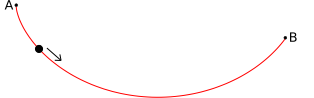
\includegraphics[scale=0.5]{images/Brachistochrone.png}
	\caption{Curva Braquistócrona}
	\label{fig:brachistochrone}
\end{figure}

\indent Este problema apenas é válido quando se consideram pares de pontos com a altura de B inferior à de A, pois caso contrário o corpo não consegue efectuar o percurso.

Leibniz, L'Hospital, Newton, e os irmãos Bernoulli apresentaram soluções analíticas.
No entanto o estudo deste problema, segundo o paradigma de agentes adaptativos, é interessante pois permite calcular uma aproximação da curva
não necessitando de ferramentas matemáticas complexas.

\indent Para cada instância do problema, um indivíduo representa uma trajectória possível. Estes individuos são avaliados segundo uma
função de aptidão que mede o tempo correspondente: quanto menor, mais apto ele é considerado.

\indent De forma a definir o o formato da trajectória, cada indivíduo é caracterizado por um conjunto de genes. Estes representam os vários
factores que contribuem para a forma da trajectória, como por exemplo coordenadas, declives, curvaturas, etc. Assim, para alterar as características
de um determinado indivíduo (fenótipo) é necessário efectuar alterações ao seu conjunto genético (genótipo). Estas alterações podem se categorizar
fundamentalmente em dois tipos:

\begin{description}
	\item[Mutation] \hfill \\ 
		Alteração ou substituição de um gene por outro de origem primariamente estocástica.
	\item[Crossover] \hfill \\ 
		Aplicação de permutações no código genético de dois ou mais indivíduos, trocando a informação genética de um para outro.
\end{description}

\cleardoublepage
\section{Implementation}
\indent \indent Durante a implementação deste projecto foram surgindo abordagens alternativas,
introduzidas tanto por erros conceptuais, como por \emph{bugs}. Estas abordagens, apesar de não estarem de acordo com
o considerado comum na àrea de Inteligência Artificial, foram demonstrando capacidade de gerar soluções adequadas ao problema.
Assim, decidimos que seria interessante efectuar uma comparação entre os resultados obtidos segundo o método tradicional, e aquele a que apelidámos \emph{Rafael-Ribeiro}. 

\subsection{Representation}
\label{subsec:representation}
\indent \indent À semelhança de outros problemas\footnote[1]{Aplicação do método do trapézio para o cálculo do integral de uma curva.}, a discretização do espaço contínuo em amostras
distintas facilita a computação numérica dos resultados. Desta forma escolhemos implementar duas formas de representação:

\begin{description}
	\item[Fixed] \hfill \\
	\label{it:fixed_representation}
		Onde a curva é aproximada por um conjunto sucessivo de segmentos de recta, definidos por pares de pontos equidistantes.
	\item[Dynamic] \hfill \\
	\label{it:dynamic_representation}
		Uma representação da mesma natureza que a anterior, apenas retirando a restrição da distância entre pontos.
\end{description}

\indent Estas duas representações foram escolhidas por serem compactas, i.e.: para cada gene apenas é necessário guardar a informação das suas coordenadas.
Note-se que no caso da representação fixa a absissa é conhecida \emph{a priori}, reduzindo assim o espaço de procura exponencialmente (em relação à dinâmica).

\indent Para além destas duas representações considerámos ainda uma terceira:

\begin{description}
	\item[NURBS] \hfill \\ 
		A curva aproximada é definida à custa dos pontos de controlo de uma NURBS\footnote[2]{Non-uniform rational basis spline.}. 
		\begin{figure}[ht]
			\centering
			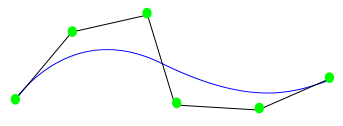
\includegraphics[scale=0.50]{images/NURBstatic.png}
			\caption{Exemplo de uma NURBS}
			\label{fig:nurbs}
		\end{figure}
\end{description}

\indent A principal vantagem desta representação é o facto de se basear em polinómios de grau superior a um, o que permite aproximar a curva desejada
com igual rigor utilizando um conjunto de pontos inferior. Desta forma o espaço de procura é mais reduzido, pelo que a convergência do algoritmo
seria esperadamente mais rápida.

\indent No entanto esta representação também apresenta os seus problemas: a avaliação da aptidão de um indivíduo depende do cálculo da derivada
desta curva, o que representa por si só um problema merecedor de uma análise profunda. 

\cleardoublepage
\subsection{Mutation Operators}
\indent \indent Um dos principais factores que contribuem para a performance de um algoritmo genético é a diversidade genética presente na população.
Desta forma, desenvolver os operadores de mutação adequados para cada problema torna-se uma tarefa crucial.
Estes actuam ao nível de cada gene e são portanto distintos para cada representação. 

\subsubsection{Fixed Representation}
\indent \indent Nesta representação o único parâmetro que se altera são as coordenadas \emph{yy} de cada gene.
Para sortear o novo valor a atribuir foi utilizada uma distribuição gaussiana (ao invés de uniforme), com o intuito 
de garantir que a evolução progenitor-filho é efectuada de forma gradual (i.e.: que o filho preserva algumas características dos
seus antecessores).

\subsubsection{Dynamic Representation}
\indent \indent Ao contrário da representação anterior, o operador de mutação para a representação dinâmica necessíta de considerar
tanto as coordenadas \emph{yy} como as \emph{xx}. Pelas razões já enunciadas, a distribuição utilizada foi novamente a gaussiana.
No entanto, uma vez que esta permite alterar a posição relativa dos pontos, é necessário efectuar um ordenamento posterior.

\indent Como estes operadores se aplicam a genes individualmente, é necessário escolher quais genes sofrem mutação.
O operador tradicional aplica uma igual probabilidade a cada gene. No entanto, segundo o paradigma biológico,
a probabilidade de erros consecutivos é mais elevada (pois a anomalia que levou à criação do primeiro erro pode ainda verificar-se).
Como achamos que esta abordagem poderia ser vantajosa para o problema em questão, decidimos implementar dois modelos de mutações adicionais:

\begin{description}
	\item[Burst] \hfill \\ 
		Onde indicamos a probabilidade de um gene ser mutado após o seu antecessor também o ser.

	\item[Partial] \hfill \\
		\label{it:partial_mutation}
		Onde por cada indivíduo são selecionados um número fixo de genes para sofer mutação.
		Este tipo de mutação é apenas aplicado para o tipo de selecção \emph{Rafael-Ribeiro}.
\end{description}
 
\cleardoublepage
\subsection{Crossover Operator}
\indent \indent O operador de recombinação distingue-se do operador de mutação na forma como tem impacto no material genético da população.
Enquanto que o operador de mutação actua sobre um único indivíduo (o que introduz novo material genético na população),
o operador de recombinação reorganiza o material genético já existente, conseguindo propagar as características entre indivíduos.
Este operador aliado a um tipo de selecção adequado (ver \ref{subsec:selection}) permite uma melhor convergência
do algoritmo.

\subsubsection{Fixed Representation}
\indent \indent Nesta representação, após o sorteio do número de pontos de recombinação (que não excede um máximo estabelecido) o operador
sorteia as coordenadas em que tais pontos de recombinação se vão aplicar, efectuando as trocas correspondentes.

\subsubsection{Dynamic Representation}
\indent \indent Dada a natureza da representação, as coordenadas sorteadas para pontos de recombinação não \emph{têm} que necessariamente existir no indivíduo.
Como tal, as coordenadas entre cada ponto de recombinação são trocadas entre si, independentemente deste processo recombinar mais ou menos genes.
Após este processo, é aplicado sobre os indivíduos com maior número de pontos (que o valor pré-definido) o operador de remoção de genes; sobre os indivíduos com menor
número de pontos é aplicado o operador de interpolação de pontos, por forma a perfazer o total de pontos do indivíduo.

\cleardoublepage
\subsection{Selection}
\label{subsec:selection}
\indent \indent Após a criação de novos descendentes é necessário efectuar uma redução no número de indivíduos.
Desta forma é possível garantir que o tamanho da população continua computacionalmente tratável e que o algoritmo convirja tendencialmente para o óptimo global.

\indent De notar que o elitismo é usualmente utilizado (excepto na selecção Rafael-Ribeiro) simultaneamente com selecção por roleta ou torneio.

\begin{description}
	\item[Elitism] \hfill \\
		Abordagem gananciosa que seleciona os melhores indivíduos da população como descendetes.

	\item[Roulette] \hfill \\
		Os indivíduos são selecionados de forma aleatória, dando maior probabilidade aos indivíduos com maior fitness.
		Para garantir esta propriedade a função de probabilidade para um indivíduo $i$ é:

		\[
			p_{i} = \frac{f_{i}}{\sum\limits_{j \in \text{Pop.}} f_{j}} \quad \text{onde} \quad f_i = \frac{1}{T_{i}} \quad (T_{i} \leftarrow \text{Tempo correspondente ao indivíduo } i)
		\]

		Neste algoritmo o mesmo elemento pode ser escolhido várias vezes,
		simulando a capacidade de um ser mais apto se conseguir reproduzir com maior frequência.

	\item[Tournament] \hfill \\ 
		Para este tipo de selecção são escolhidos aleatoriamente N indivíduos, dos quais apenas o mais apto é escolhido.
		Após esta selecção todos os elementos participantes no torneio são devolvidos à população.

	\item[Rafael-Ribeiro] \hfill \\
		Nesta abordagem implementa-se em conjunto a selecção por elitismo e por torneio, mas ao contrário da abordagem tradicional
		esta é aplicada não só para selecionar os progenitores, mas também para selecionar que indivíduos da população inteira (pais e filhos)
		sobrevivem para a próxima iteração. Do ponto de vista que apenas alguns indivíduos são alterados, este tipo de selecção pode ser considerada \emph{Steady-State}.

\end{description}

\cleardoublepage

\section{Experiments}
\label{sec:experiments}
\indent \indent Os resultados obtidos com algoritmos genéticos dependem intrinsecamente dos parâmetros com os quais são executados
(representação, modo de selecção, percentagem de elitismo, ...). Assim, para uma correcta análise do seu comportamento
torna-se necessário analisar as várias combinações. Como tal, para cada parâmetro foram escolhidos 2 ou 3 valores.
Enumeram-se de seguida as variações.

\begin{description}
	\item [Points set] \hfill \\
		\indent Foram utilizados dois conjuntos de pontos (inicial e final) para averiguar a correcta convergência em diferentes casos.
			\begin{description}
				\item \[ P_{init} = (0.0, 3.0),\quad P_{final} = (4.0, 2.0) \]
				\item \[ P_{init} = (0.0, 3.0),\quad P_{final} = (4.0, 2.8) \]
			\end{description}
	\item [Representation] \hfill \\
		\indent Foram testados os tipos de representação já mencionados em \ref{subsec:representation}.
	\item [Selection] \hfill \\
		\indent Foram testados os tipos de selecção já mencionados em \ref{subsec:selection}. No entanto, o elitismo foi variado em simultâneo com
		as selecções Torneio, Roleta e Rafael-Ribeiro, uma vez que são aplicadas em fases diferentes do algoritmo.
	\begin{description}
		\item [Elitismo] \hfill \\
			\indent Os valores utilizados foram 5\% e 20\%. Pensamos que 5\% é um valor adequado dado o contexto do problema; 20\%
			foi escolhido para averiguar se a convergência do algoritmo para um óptimo global ainda se manteria.
	\end{description}
	\item [No. of points] \hfill \\
		\indent Os valores utilizados para o número de pontos foram 15 e 30; estes valores foram escolhidos após experimentação, dado que concluímos
		que um maior número de pontos torna o espaço de procura demasiado extenso.
	\item [Population size] \hfill \\
		\indent Para os tamanhos de população foram utilizados os valores de 25, 50 e 100 indivíduos. %TODO Justificar como sendo valores adequados (após experimentação)?
	\item [Crossover probability] \hfill \\
		\indent Para a probabilidade de ocorrência de recombinação foram escolhidos os valores de 0\% e 35\%. A escolha do valor de 35\% ocorreu após
		experimentação; já o valor de 0\% foi escolhido para testar os resultados em que a única variação/propagação do material genético da população se deve
		a mutações aliadas a métodos de selecção. De notar que quando a probabilidade de recombinação é 0\% o parâmetro relativo ao número de pontos de recombinação
		não é aplicado.
	\item [Crossover points] \hfill \\
		\indent Os dois valores de pontos de recombinação utilizados foram 2 e 5. %TODO Existe justificação?
	\item [Mutation probability] \hfill \\
		\indent Os valores utilizados para a probabilidade de mutação foram 5\% e 25\%. %TODO Existe justificação?
\end{description}

\cleardoublepage

\section{Validation}
\indent \indent Para validar o comportamento do Agente, cada combinação de parâmetros foi executada 30 vezes com seeds diferentes;
tal garante que a natureza estocástica do algoritmo fica evidenciada ao garantir que os testes são, de facto, diferentes.

Após a conclusão dos testes, foi calculado o desvio-padrão entre as 30 simulações,
para averiguar se os resultados obtidos não representavam apenas um caso de sorte.

Tal como se pode verificar na última coluna da tabela de resultados (Secção \ref{tab:results}), o desvio-padrão entre as 30 simulações para cada combinação de parâmetros
é bastante reduzido\footnote[1]{São excepção os testes onde a probabilidade de recombinação é 0.00\%, pois a ausência deste operador torna a evolução individual,
não tomando partido das soluções obtidas pelos outros indivíduos da população.}, o que comprova a sua consistência e robustez.

\cleardoublepage
\section{Result Analysis}

\cleardoublepage
\subsection{Representation}
\begin{figure}[ht]
	\centering
	\subfloat[200 iterations]{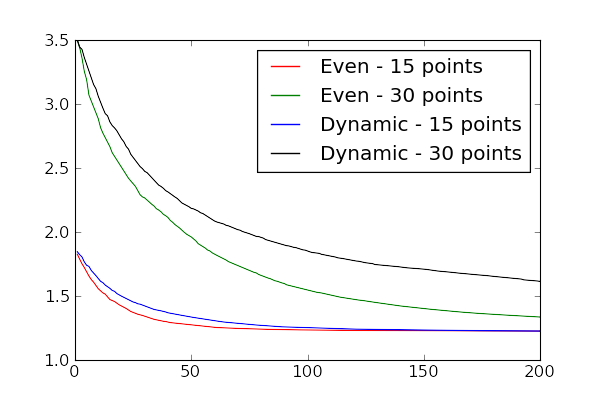
\includegraphics[width=0.3\textwidth]{images/evolution_200.png}}
	\subfloat[2000 iterations]{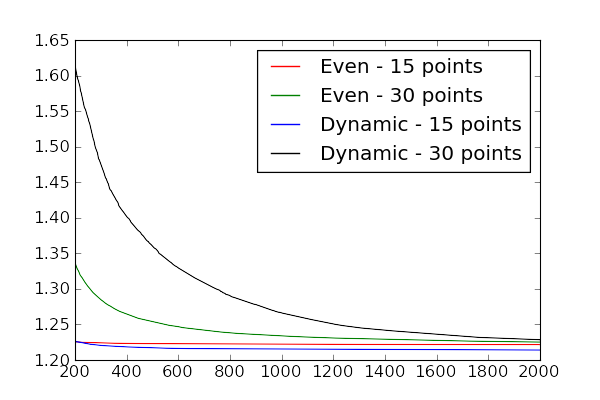
\includegraphics[width=0.3\textwidth]{images/evolution_2000.png}}
	\subfloat[5000 iterations]{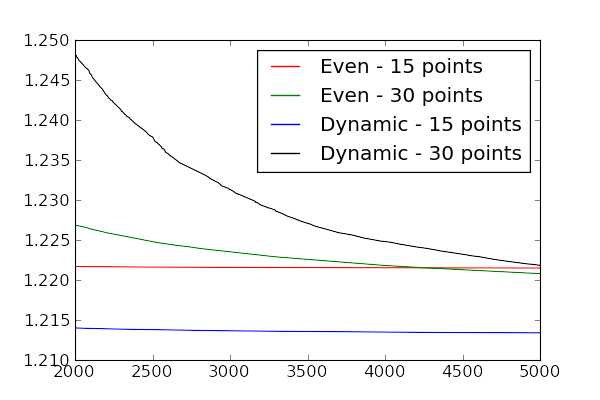
\includegraphics[width=0.3\textwidth]{images/evolution_5000.png}}
	\caption{Fitness evolution}
\end{figure}

\indent \indent Como é possível observar pelos gráficos (ou constatar nas tabelas da secção \ref{sec:fitness_by_representation}), a representação fixa converge mais rapidamente para o óptimo global
(permitido por esta) do que a representação dinâmica. Esta propriedade justifica-se pelo facto do espaço de procura ser
mais reduzido. No entanto, por essa mesma razão, o valor final de aptidão obtido é inferior ao obtido com a representação dinâmica.
Verifica-se experimentalmente que o número de iterações a partir do qual compensa utilizar uma representação dinâmica
depende do número de pontos utilizado, bem como dos pontos iniciais e finais.

\indent Outra propriedade merecedora de análise é a média das aptidões dos melhores indíviduos para cada representação.
Como podemos observar na tabela correspondente \ref{sec:fitness_by_representation}, a média é inferior para a representação igualmente espaçada,
o que nos indica que esta é mais consistente (i.e.: menos sensível a ajustes de parâmetros). 

\cleardoublepage

\subsection{Selection}
\indent \indent Como é possível verificar na tabela da secção \ref{sec:fitness_by_selection}, a "selecção"\footnote[1]{De relembrar o leitor de que o algoritmo Rafael-Ribeiro
apresenta um funcionamento diferente ao nível das mutações, não sendo assim classificável como puramente um método de selecção.} Rafael-Ribeiro é claramente
superior na representação de pontos igualmente espaçados. Tal deve-se à sua abordagem semelhante a Estado Estável, isto é, estocasticamente a percentagem de
indivíduos de elevada aptidão que permanece na geração seguinte é superior; este facto favorece o tipo de mutação utilizado (ver secção \ref{it:partial_mutation}),
o que força uma melhor convergência do algoritmo ao permitir fugas de óptimos locais.

\indent Na mesma tabela da secção \ref{sec:fitness_by_selection} é possível observar que a representação dinamicamente espaçada obtém melhores resultados com a Roleta.
Tal se deve ao facto de o seu espaço de procura ser exponencialmente maior do que o da representação igualmente espaçada. Assim, a Roleta ao favorecer a diversidade
genética permite uma melhor exploração do espaço de procura ao permitir que indivíduos menos bons permaneçam nas gerações seguintes.

\cleardoublepage

\subsection{Crossover}
\indent \indent Tal como indicado na secção \ref{sec:experiments} o parâmetro de recombinação a 0\% foi experimentado com o
intuito de verificar o impacto do operador de recombinação. Esta situação foi comprovada experimentalmente e pode ser observada em \ref{sec:crossover_on_off}.

\indent Por outro lado o número de pontos de recombinação utilizados demonstrou ser um factor irrelevante à performance do algoritmo.

\cleardoublepage
\subsection{Population Size}
\indent \indent Os dados presentes na tabela \ref{sec:results} indicam, tal como esperado, que quanto maior a população melhores
os resultados. No entanto, uma vez que aumentar o tamanho da população aumenta necessáriamente
o tempo de computação de cada iteração, torna-se interessante analisar mais detalhadamente este \emph{trade-off}.

\indent Como é possível observar na tabela \ref{sec:fitness_by_population_size}, os resultados obtidos com uma
população de \emph{n} indivíduos em \emph{m} iterações são ligeiramente melhores que os obtidos
com uma população com o dobro do tamanho em metade do tempo. Esta convergência mais rápida justifica-se
pelo facto de existirem menos indivíduos a seguirem caminhos evolucionários semelhantes. No entanto, por esta
mesma razão a resistência a óptimos locais é inferior.
 
\cleardoublepage

\subsection{Mutation}
\indent \indent TODO % TODO FIXME

\subsubsection{Mutation burst}
\indent \indent TODO % TODO FIXME

\cleardoublepage

\eject \pdfpagewidth=594.0mm \pdfpageheight=420.0mm
\paperwidth=594.0mm
\paperheight=420.0mm

\section{Attachments}

\subsection{Results' Table}
\label{sec:results}
\begin{center}
	\begin{longtable}{ | c | c | c | c | c | c | c | c | c | c | c | c | c | c | c | c | c | }
	\hline
	\textbf{Points set}	&	\textbf{Representation}	&	\textbf{Selection Type}	&	\textbf{No. pts.}	&	\textbf{Pop. size}	&	\textbf{Elitism  (\%)}	&	\textbf{Crossover Prob. (\%)}	&	\textbf{No. pts. Crossover}	&	\textbf{Prob. Mutation (\%)}	&	\textbf{Best (20)}	&	\textbf{Best (100)}	&	\textbf{Best (1000)}	&	\textbf{Best (2000)}	&	\textbf{Average (2000)}	&	\textbf{Worst (2000)}	&	\textbf{Std. Dev. (2000, Pop.)}	&	\textbf{Std. Dev. x100 (2000, 30 runs)} \\
	\hline
	\hline
	1	&	Dynamic	&	Tournament	&	15	&	25	&	5.00	&	0.00	&	NA	&	5.00	&	1.7798555	&	1.3804207	&	1.2214826	&	1.2171368	&	1.2855872	&	1.8891135	&	0.1423133	&	0.1569723 \\
	\hline
	1	&	Dynamic	&	Tournament	&	15	&	25	&	5.00	&	0.00	&	NA	&	25.00	&	1.6387113	&	1.3374381	&	1.2294197	&	1.2240526	&	1.5092776	&	1.9289822	&	0.1856915	&	0.5851234 \\
	\hline
	1	&	Dynamic	&	Tournament	&	15	&	25	&	5.00	&	35.00	&	2	&	5.00	&	1.7645611	&	1.3846251	&	1.2235878	&	1.2178209	&	1.2755522	&	1.5378397	&	0.0731764	&	0.2559497 \\
	\hline
	1	&	Dynamic	&	Tournament	&	15	&	25	&	5.00	&	35.00	&	2	&	25.00	&	1.6366198	&	1.3489135	&	1.2306325	&	1.2241706	&	1.5815125	&	3.2559805	&	0.4413373	&	0.7620405 \\
	\hline
	1	&	Dynamic	&	Tournament	&	15	&	25	&	5.00	&	35.00	&	5	&	5.00	&	1.7549878	&	1.3941534	&	1.2222179	&	1.2179503	&	1.2753718	&	1.5528651	&	0.0755826	&	0.2365574 \\
	\hline
	1	&	Dynamic	&	Tournament	&	15	&	25	&	5.00	&	35.00	&	5	&	25.00	&	1.5997140	&	1.3169590	&	1.2312039	&	1.2253416	&	1.5561979	&	2.8622221	&	0.3605938	&	0.6181510 \\
	\hline
	1	&	Dynamic	&	Tournament	&	15	&	25	&	20.00	&	0.00	&	NA	&	5.00	&	1.7071056	&	1.3596559	&	1.2178007	&	1.2153561	&	1.2384174	&	1.4464642	&	0.0544712	&	0.1049954 \\
	\hline
	1	&	Dynamic	&	Tournament	&	15	&	25	&	20.00	&	0.00	&	NA	&	25.00	&	1.5775374	&	1.2914149	&	1.2230546	&	1.2194394	&	1.3333207	&	1.6977337	&	0.1257296	&	0.2242895 \\
	\hline
	1	&	Dynamic	&	Tournament	&	15	&	25	&	20.00	&	35.00	&	2	&	5.00	&	1.7568935	&	1.3711726	&	1.2181654	&	1.2152563	&	1.2435227	&	1.5839707	&	0.0801040	&	0.0964408 \\
	\hline
	1	&	Dynamic	&	Tournament	&	15	&	25	&	20.00	&	35.00	&	2	&	25.00	&	1.5664255	&	1.2805528	&	1.2250549	&	1.2206995	&	1.3494917	&	1.7543654	&	0.1435915	&	0.4044988 \\
	\hline
	1	&	Dynamic	&	Tournament	&	15	&	25	&	20.00	&	35.00	&	5	&	5.00	&	1.7142195	&	1.3411961	&	1.2175074	&	1.2151081	&	1.2483471	&	1.5921128	&	0.0860409	&	0.0938125 \\
	\hline
	1	&	Dynamic	&	Tournament	&	15	&	25	&	20.00	&	35.00	&	5	&	25.00	&	1.5924041	&	1.2946479	&	1.2234791	&	1.2193236	&	1.3530618	&	1.8036510	&	0.1517908	&	0.3063623 \\
	\hline
	1	&	Dynamic	&	Tournament	&	15	&	50	&	5.00	&	0.00	&	NA	&	5.00	&	1.6779650	&	1.3591788	&	1.2239797	&	1.2182432	&	1.3901535	&	1.8152864	&	0.1432619	&	0.3508536 \\
	\hline
	1	&	Dynamic	&	Tournament	&	15	&	50	&	5.00	&	0.00	&	NA	&	25.00	&	1.5739769	&	1.3269143	&	1.2310873	&	1.2234359	&	1.7627173	&	2.4092700	&	0.2931448	&	0.4940614 \\
	\hline
	1	&	Dynamic	&	Tournament	&	15	&	50	&	5.00	&	35.00	&	2	&	5.00	&	1.6574976	&	1.3652564	&	1.2220822	&	1.2180924	&	1.4018081	&	2.2147800	&	0.1984693	&	0.3499979 \\
	\hline
	1	&	Dynamic	&	Tournament	&	15	&	50	&	5.00	&	35.00	&	2	&	25.00	&	1.5733395	&	1.3194227	&	1.2316545	&	1.2245416	&	1.8001901	&	4.0780631	&	0.5095846	&	0.8556297 \\
	\hline
	1	&	Dynamic	&	Tournament	&	15	&	50	&	5.00	&	35.00	&	5	&	5.00	&	1.6570812	&	1.3408675	&	1.2210690	&	1.2172407	&	1.4015002	&	2.1589754	&	0.1863246	&	0.2608487 \\
	\hline
	1	&	Dynamic	&	Tournament	&	15	&	50	&	5.00	&	35.00	&	5	&	25.00	&	1.5473851	&	1.3247167	&	1.2318544	&	1.2243604	&	1.7338216	&	2.7922778	&	0.3339150	&	0.6634347 \\
	\hline
	1	&	Dynamic	&	Tournament	&	15	&	50	&	20.00	&	0.00	&	NA	&	5.00	&	1.6078798	&	1.2990023	&	1.2161943	&	1.2144174	&	1.2460124	&	1.6751434	&	0.0830522	&	0.0608947 \\
	\hline
	1	&	Dynamic	&	Tournament	&	15	&	50	&	20.00	&	0.00	&	NA	&	25.00	&	1.4786964	&	1.2645791	&	1.2217304	&	1.2184489	&	1.4166767	&	2.7871974	&	0.2909448	&	0.3414112 \\
	\hline
	1	&	Dynamic	&	Tournament	&	15	&	50	&	20.00	&	35.00	&	2	&	5.00	&	1.5905558	&	1.3096392	&	1.2162614	&	1.2144527	&	1.2530232	&	1.9220403	&	0.1190049	&	0.0574027 \\
	\hline
	1	&	Dynamic	&	Tournament	&	15	&	50	&	20.00	&	35.00	&	2	&	25.00	&	1.4909638	&	1.2580901	&	1.2204253	&	1.2180191	&	1.3972693	&	2.6893642	&	0.2659871	&	0.2524264 \\
	\hline
	1	&	Dynamic	&	Tournament	&	15	&	50	&	20.00	&	35.00	&	5	&	5.00	&	1.5983842	&	1.3041431	&	1.2168150	&	1.2147173	&	1.2497317	&	1.7564688	&	0.0948583	&	0.0787589 \\
	\hline
	1	&	Dynamic	&	Tournament	&	15	&	50	&	20.00	&	35.00	&	5	&	25.00	&	1.5005366	&	1.2666354	&	1.2207167	&	1.2176385	&	1.4062357	&	2.7415784	&	0.2743122	&	0.2207026 \\
	\hline
	1	&	Dynamic	&	Tournament	&	15	&	100	&	5.00	&	0.00	&	NA	&	5.00	&	1.5584232	&	1.2977242	&	1.2177620	&	1.2151850	&	1.3377928	&	2.3506955	&	0.1625919	&	0.0993585 \\
	\hline
	1	&	Dynamic	&	Tournament	&	15	&	100	&	5.00	&	0.00	&	NA	&	25.00	&	1.4597030	&	1.2617386	&	1.2223083	&	1.2189487	&	1.6976760	&	3.9941744	&	0.4365012	&	0.2988285 \\
	\hline
	1	&	Dynamic	&	Tournament	&	15	&	100	&	5.00	&	35.00	&	2	&	5.00	&	1.5430401	&	1.2867505	&	1.2176236	&	1.2152363	&	1.3303994	&	1.9426754	&	0.1261230	&	0.1099206 \\
	\hline
	1	&	Dynamic	&	Tournament	&	15	&	100	&	5.00	&	35.00	&	2	&	25.00	&	1.4803913	&	1.2657400	&	1.2234430	&	1.2193863	&	1.6750848	&	4.7410434	&	0.4686266	&	0.3027827 \\
	\hline
	1	&	Dynamic	&	Tournament	&	15	&	100	&	5.00	&	35.00	&	5	&	5.00	&	1.5515495	&	1.2900368	&	1.2184431	&	1.2153366	&	1.3438610	&	1.9015783	&	0.1250422	&	0.0949568 \\
	\hline
	1	&	Dynamic	&	Tournament	&	15	&	100	&	5.00	&	35.00	&	5	&	25.00	&	1.4731484	&	1.2656088	&	1.2224566	&	1.2196624	&	1.6389763	&	3.0345345	&	0.3051621	&	0.3502439 \\
	\hline
	1	&	Dynamic	&	Tournament	&	15	&	100	&	20.00	&	0.00	&	NA	&	5.00	&	1.5089657	&	1.2591590	&	1.2152843	&	1.2141346	&	1.2499208	&	1.7710180	&	0.0934463	&	0.0664633 \\
	\hline
	1	&	Dynamic	&	Tournament	&	15	&	100	&	20.00	&	0.00	&	NA	&	25.00	&	1.4306861	&	1.2447508	&	1.2181126	&	1.2162282	&	1.4217654	&	4.1642367	&	0.3837596	&	0.1675580 \\
	\hline
	1	&	Dynamic	&	Tournament	&	15	&	100	&	20.00	&	35.00	&	2	&	5.00	&	1.5204479	&	1.2623009	&	1.2153587	&	1.2140487	&	1.2472616	&	1.8195834	&	0.0910645	&	0.0653385 \\
	\hline
	1	&	Dynamic	&	Tournament	&	15	&	100	&	20.00	&	35.00	&	2	&	25.00	&	1.4389591	&	1.2487813	&	1.2186170	&	1.2166224	&	1.4005038	&	3.1380292	&	0.2733357	&	0.1470783 \\
	\hline
	1	&	Dynamic	&	Tournament	&	15	&	100	&	20.00	&	35.00	&	5	&	5.00	&	1.5048529	&	1.2673824	&	1.2153698	&	1.2140683	&	1.2517682	&	2.1992441	&	0.1275911	&	0.0402102 \\
	\hline
	1	&	Dynamic	&	Tournament	&	15	&	100	&	20.00	&	35.00	&	5	&	25.00	&	1.4394328	&	1.2482233	&	1.2193379	&	1.2170282	&	1.3887502	&	2.3375056	&	0.1933840	&	0.1852128 \\
	\hline
	1	&	Dynamic	&	Tournament	&	30	&	25	&	5.00	&	0.00	&	NA	&	5.00	&	3.0241153	&	2.2870420	&	1.5261449	&	1.3493051	&	1.5935519	&	2.0557476	&	0.1858032	&	7.8105710 \\
	\hline
	1	&	Dynamic	&	Tournament	&	30	&	25	&	5.00	&	0.00	&	NA	&	25.00	&	2.9892652	&	2.3966830	&	1.8011931	&	1.6516420	&	2.8222093	&	3.9452314	&	0.5841092	&	18.5965986 \\
	\hline
	1	&	Dynamic	&	Tournament	&	30	&	25	&	5.00	&	35.00	&	2	&	5.00	&	2.9944279	&	2.2714349	&	1.5017791	&	1.3624134	&	1.6238496	&	2.1611009	&	0.2061994	&	10.1997876 \\
	\hline
	1	&	Dynamic	&	Tournament	&	30	&	25	&	5.00	&	35.00	&	2	&	25.00	&	2.9637315	&	2.4028335	&	1.7987249	&	1.6562247	&	2.8073140	&	4.2412314	&	0.6476271	&	20.1348564 \\
	\hline
	1	&	Dynamic	&	Tournament	&	30	&	25	&	5.00	&	35.00	&	5	&	5.00	&	3.0334155	&	2.3078157	&	1.5169478	&	1.3662690	&	1.6250130	&	2.0575869	&	0.1896045	&	8.5788800 \\
	\hline
	1	&	Dynamic	&	Tournament	&	30	&	25	&	5.00	&	35.00	&	5	&	25.00	&	3.0521300	&	2.3782740	&	1.7726390	&	1.6618767	&	2.7643008	&	3.8716787	&	0.5660606	&	21.7655209 \\
	\hline
	1	&	Dynamic	&	Tournament	&	30	&	25	&	20.00	&	0.00	&	NA	&	5.00	&	2.9539978	&	2.1024998	&	1.3519152	&	1.2628652	&	1.3420289	&	1.8731640	&	0.1413552	&	3.6082740 \\
	\hline
	1	&	Dynamic	&	Tournament	&	30	&	25	&	20.00	&	0.00	&	NA	&	25.00	&	2.8256159	&	2.1885145	&	1.6509152	&	1.5287695	&	2.0324691	&	3.3636243	&	0.4852465	&	17.7621368 \\
	\hline
	1	&	Dynamic	&	Tournament	&	30	&	25	&	20.00	&	35.00	&	2	&	5.00	&	2.9140885	&	2.1317807	&	1.3912177	&	1.2900100	&	1.3650007	&	1.7495199	&	0.1145554	&	5.7359827 \\
	\hline
	1	&	Dynamic	&	Tournament	&	30	&	25	&	20.00	&	35.00	&	2	&	25.00	&	2.8855914	&	2.1740878	&	1.5921175	&	1.4947861	&	1.9830452	&	3.4054299	&	0.4880600	&	14.9423265 \\
	\hline
	1	&	Dynamic	&	Tournament	&	30	&	25	&	20.00	&	35.00	&	5	&	5.00	&	2.9489919	&	2.1012636	&	1.3534723	&	1.2743137	&	1.3479058	&	1.7043310	&	0.1063730	&	4.6961729 \\
	\hline
	1	&	Dynamic	&	Tournament	&	30	&	25	&	20.00	&	35.00	&	5	&	25.00	&	2.8911136	&	2.1482890	&	1.5624525	&	1.4742001	&	1.9301330	&	2.6171929	&	0.3439067	&	14.1575000 \\
	\hline
	1	&	Dynamic	&	Tournament	&	30	&	50	&	5.00	&	0.00	&	NA	&	5.00	&	2.9820616	&	2.1976345	&	1.4638068	&	1.3451448	&	1.9028023	&	3.1948918	&	0.4139098	&	8.7382751 \\
	\hline
	1	&	Dynamic	&	Tournament	&	30	&	50	&	5.00	&	0.00	&	NA	&	25.00	&	3.0034802	&	2.3564119	&	1.7758596	&	1.6488573	&	3.2832022	&	4.4628544	&	0.6538322	&	18.0427582 \\
	\hline
	1	&	Dynamic	&	Tournament	&	30	&	50	&	5.00	&	35.00	&	2	&	5.00	&	2.9723681	&	2.2320806	&	1.4687581	&	1.3444392	&	1.9168218	&	2.7218863	&	0.3499373	&	7.4816034 \\
	\hline
	1	&	Dynamic	&	Tournament	&	30	&	50	&	5.00	&	35.00	&	2	&	25.00	&	2.9259580	&	2.3955879	&	1.8552572	&	1.7427870	&	3.5077731	&	6.1051042	&	0.8377945	&	22.4558609 \\
	\hline
	1	&	Dynamic	&	Tournament	&	30	&	50	&	5.00	&	35.00	&	5	&	5.00	&	3.0008071	&	2.2872974	&	1.5014871	&	1.3553037	&	1.9173880	&	2.7280623	&	0.3427520	&	9.9224450 \\
	\hline
	1	&	Dynamic	&	Tournament	&	30	&	50	&	5.00	&	35.00	&	5	&	25.00	&	2.9592536	&	2.3321408	&	1.7415598	&	1.6248364	&	3.2725527	&	4.6691223	&	0.6864720	&	16.4034541 \\
	\hline
	1	&	Dynamic	&	Tournament	&	30	&	50	&	20.00	&	0.00	&	NA	&	5.00	&	2.7942350	&	1.9568596	&	1.3315192	&	1.2539519	&	1.3404724	&	1.9544724	&	0.1320934	&	2.4978841 \\
	\hline
	1	&	Dynamic	&	Tournament	&	30	&	50	&	20.00	&	0.00	&	NA	&	25.00	&	2.7053609	&	1.9250811	&	1.4502105	&	1.3762398	&	1.9260496	&	4.0336877	&	0.5569000	&	8.8982337 \\
	\hline
	1	&	Dynamic	&	Tournament	&	30	&	50	&	20.00	&	35.00	&	2	&	5.00	&	2.7947838	&	1.9768370	&	1.3333488	&	1.2610420	&	1.3453404	&	1.7543229	&	0.1055524	&	3.8732595 \\
	\hline
	1	&	Dynamic	&	Tournament	&	30	&	50	&	20.00	&	35.00	&	2	&	25.00	&	2.7260588	&	1.9821525	&	1.4704425	&	1.3956011	&	1.8817648	&	2.6872210	&	0.3542646	&	10.2229845 \\
	\hline
	1	&	Dynamic	&	Tournament	&	30	&	50	&	20.00	&	35.00	&	5	&	5.00	&	2.8228348	&	1.9838148	&	1.3309642	&	1.2555107	&	1.3407083	&	1.8394806	&	0.1141787	&	3.1595486 \\
	\hline
	1	&	Dynamic	&	Tournament	&	30	&	50	&	20.00	&	35.00	&	5	&	25.00	&	2.7117558	&	1.9953746	&	1.5032434	&	1.4207996	&	1.9737368	&	3.5947762	&	0.4675957	&	13.6142756 \\
	\hline
	1	&	Dynamic	&	Tournament	&	30	&	100	&	5.00	&	0.00	&	NA	&	5.00	&	2.7603940	&	1.9784741	&	1.3422039	&	1.2772740	&	1.6166756	&	2.5409931	&	0.2532344	&	4.8995051 \\
	\hline
	1	&	Dynamic	&	Tournament	&	30	&	100	&	5.00	&	0.00	&	NA	&	25.00	&	2.7162829	&	2.0087901	&	1.5505925	&	1.4656556	&	2.6675271	&	4.3925622	&	0.5927422	&	15.8928720 \\
	\hline
	1	&	Dynamic	&	Tournament	&	30	&	100	&	5.00	&	35.00	&	2	&	5.00	&	2.7399697	&	2.0250188	&	1.3517838	&	1.2687510	&	1.5949186	&	2.4785520	&	0.2454454	&	4.7645855 \\
	\hline
	1	&	Dynamic	&	Tournament	&	30	&	100	&	5.00	&	35.00	&	2	&	25.00	&	2.6135124	&	1.9763409	&	1.5522914	&	1.4706218	&	2.7402147	&	4.8428890	&	0.6463274	&	15.8192247 \\
	\hline
	1	&	Dynamic	&	Tournament	&	30	&	100	&	5.00	&	35.00	&	5	&	5.00	&	2.7861186	&	1.9806727	&	1.3340448	&	1.2654976	&	1.6121063	&	2.4439884	&	0.2486804	&	4.4538031 \\
	\hline
	1	&	Dynamic	&	Tournament	&	30	&	100	&	5.00	&	35.00	&	5	&	25.00	&	2.7095274	&	2.0570141	&	1.4825159	&	1.4073239	&	2.5495027	&	3.7207713	&	0.5420656	&	11.4028266 \\
	\hline
	1	&	Dynamic	&	Tournament	&	30	&	100	&	20.00	&	0.00	&	NA	&	5.00	&	2.6078851	&	1.8262564	&	1.2911006	&	1.2391886	&	1.3222918	&	1.9202444	&	0.1177234	&	1.8183417 \\
	\hline
	1	&	Dynamic	&	Tournament	&	30	&	100	&	20.00	&	0.00	&	NA	&	25.00	&	2.5086127	&	1.7929367	&	1.3918626	&	1.3352990	&	1.8102752	&	3.2678144	&	0.3980121	&	8.6783465 \\
	\hline
	1	&	Dynamic	&	Tournament	&	30	&	100	&	20.00	&	35.00	&	2	&	5.00	&	2.6296208	&	1.8270909	&	1.2817181	&	1.2333926	&	1.3138706	&	1.8325179	&	0.1093286	&	1.9645085 \\
	\hline
	1	&	Dynamic	&	Tournament	&	30	&	100	&	20.00	&	35.00	&	2	&	25.00	&	2.5614479	&	1.8230046	&	1.4073011	&	1.3538573	&	1.8214754	&	4.0144986	&	0.4419204	&	9.0195337 \\
	\hline
	1	&	Dynamic	&	Tournament	&	30	&	100	&	20.00	&	35.00	&	5	&	5.00	&	2.6274094	&	1.8301547	&	1.2899317	&	1.2388849	&	1.3222765	&	2.0995080	&	0.1304264	&	1.8085610 \\
	\hline
	1	&	Dynamic	&	Tournament	&	30	&	100	&	20.00	&	35.00	&	5	&	25.00	&	2.5075852	&	1.7811631	&	1.3936121	&	1.3454511	&	1.8009246	&	3.1117900	&	0.3667037	&	8.3174459 \\
	\hline
	1	&	Dynamic	&	Roulette	&	15	&	25	&	5.00	&	0.00	&	NA	&	5.00	&	1.7428558	&	1.3907379	&	1.2221460	&	1.2176776	&	1.2831480	&	1.6135393	&	0.0896902	&	0.2221814 \\
	\hline
	1	&	Dynamic	&	Roulette	&	15	&	25	&	5.00	&	0.00	&	NA	&	25.00	&	1.6270911	&	1.3158784	&	1.2312508	&	1.2233814	&	1.5787696	&	3.1214934	&	0.4123084	&	0.5164064 \\
	\hline
	1	&	Dynamic	&	Roulette	&	15	&	25	&	5.00	&	35.00	&	2	&	5.00	&	1.7616388	&	1.4037228	&	1.2223646	&	1.2174774	&	1.2730297	&	1.5881841	&	0.0832034	&	0.1910814 \\
	\hline
	1	&	Dynamic	&	Roulette	&	15	&	25	&	5.00	&	35.00	&	2	&	25.00	&	1.6398489	&	1.3389605	&	1.2290112	&	1.2235723	&	1.5438479	&	2.7500535	&	0.3435471	&	0.5140365 \\
	\hline
	1	&	Dynamic	&	Roulette	&	15	&	25	&	5.00	&	35.00	&	5	&	5.00	&	1.7216297	&	1.3608354	&	1.2208705	&	1.2172250	&	1.3037182	&	2.2094351	&	0.2048888	&	0.2008811 \\
	\hline
	1	&	Dynamic	&	Roulette	&	15	&	25	&	5.00	&	35.00	&	5	&	25.00	&	1.5875229	&	1.3263148	&	1.2308108	&	1.2243531	&	1.5789210	&	2.6740883	&	0.3308117	&	0.5167461 \\
	\hline
	1	&	Dynamic	&	Roulette	&	15	&	25	&	20.00	&	0.00	&	NA	&	5.00	&	1.7484987	&	1.3541369	&	1.2178021	&	1.2151325	&	1.2505549	&	1.7122481	&	0.1055554	&	0.0790360 \\
	\hline
	1	&	Dynamic	&	Roulette	&	15	&	25	&	20.00	&	0.00	&	NA	&	25.00	&	1.5812460	&	1.2853418	&	1.2239918	&	1.2203170	&	1.3649368	&	2.2403135	&	0.2316100	&	0.4082052 \\
	\hline
	1	&	Dynamic	&	Roulette	&	15	&	25	&	20.00	&	35.00	&	2	&	5.00	&	1.7461313	&	1.3813756	&	1.2180799	&	1.2152846	&	1.2393712	&	1.4777937	&	0.0602246	&	0.0709448 \\
	\hline
	1	&	Dynamic	&	Roulette	&	15	&	25	&	20.00	&	35.00	&	2	&	25.00	&	1.5956923	&	1.2951400	&	1.2244794	&	1.2201828	&	1.3511049	&	1.8064734	&	0.1522716	&	0.4562409 \\
	\hline
	1	&	Dynamic	&	Roulette	&	15	&	25	&	20.00	&	35.00	&	5	&	5.00	&	1.7280689	&	1.3699736	&	1.2184602	&	1.2153689	&	1.2391900	&	1.4836848	&	0.0613522	&	0.1093037 \\
	\hline
	1	&	Dynamic	&	Roulette	&	15	&	25	&	20.00	&	35.00	&	5	&	25.00	&	1.5821089	&	1.3081968	&	1.2232304	&	1.2192104	&	1.3500189	&	1.7992047	&	0.1496290	&	0.2755991 \\
	\hline
	1	&	Dynamic	&	Roulette	&	15	&	50	&	5.00	&	0.00	&	NA	&	5.00	&	1.6627745	&	1.3503424	&	1.2222896	&	1.2178707	&	1.3903998	&	1.7328154	&	0.1301884	&	0.2224996 \\
	\hline
	1	&	Dynamic	&	Roulette	&	15	&	50	&	5.00	&	0.00	&	NA	&	25.00	&	1.5484784	&	1.3105168	&	1.2295210	&	1.2238031	&	1.8289541	&	4.6330684	&	0.5947717	&	0.5005507 \\
	\hline
	1	&	Dynamic	&	Roulette	&	15	&	50	&	5.00	&	35.00	&	2	&	5.00	&	1.6581429	&	1.3723184	&	1.2220793	&	1.2176520	&	1.3985260	&	1.8241810	&	0.1434455	&	0.1940176 \\
	\hline
	1	&	Dynamic	&	Roulette	&	15	&	50	&	5.00	&	35.00	&	2	&	25.00	&	1.5532844	&	1.3116116	&	1.2301845	&	1.2244249	&	1.7833691	&	3.0999511	&	0.3738119	&	0.5251096 \\
	\hline
	1	&	Dynamic	&	Roulette	&	15	&	50	&	5.00	&	35.00	&	5	&	5.00	&	1.6762995	&	1.3566805	&	1.2205564	&	1.2170021	&	1.3974064	&	1.8765936	&	0.1515107	&	0.2569220 \\
	\hline
	1	&	Dynamic	&	Roulette	&	15	&	50	&	5.00	&	35.00	&	5	&	25.00	&	1.5775049	&	1.3271575	&	1.2321838	&	1.2245138	&	1.7865066	&	3.6395958	&	0.4422532	&	0.5792444 \\
	\hline
	1	&	Dynamic	&	Roulette	&	15	&	50	&	20.00	&	0.00	&	NA	&	5.00	&	1.5762381	&	1.2945880	&	1.2166823	&	1.2147015	&	1.2507886	&	1.8021717	&	0.1037473	&	0.0723439 \\
	\hline
	1	&	Dynamic	&	Roulette	&	15	&	50	&	20.00	&	0.00	&	NA	&	25.00	&	1.4779650	&	1.2647266	&	1.2215084	&	1.2184853	&	1.3941109	&	2.6456148	&	0.2533046	&	0.2440008 \\
	\hline
	1	&	Dynamic	&	Roulette	&	15	&	50	&	20.00	&	35.00	&	2	&	5.00	&	1.5808428	&	1.2940802	&	1.2166121	&	1.2147142	&	1.2480274	&	1.7203776	&	0.0891606	&	0.0833979 \\
	\hline
	1	&	Dynamic	&	Roulette	&	15	&	50	&	20.00	&	35.00	&	2	&	25.00	&	1.4796395	&	1.2599873	&	1.2209803	&	1.2182362	&	1.3912172	&	2.1360482	&	0.1890859	&	0.3058145 \\
	\hline
	1	&	Dynamic	&	Roulette	&	15	&	50	&	20.00	&	35.00	&	5	&	5.00	&	1.5805124	&	1.3077502	&	1.2164494	&	1.2146498	&	1.2492966	&	1.7803488	&	0.0980238	&	0.0822618 \\
	\hline
	1	&	Dynamic	&	Roulette	&	15	&	50	&	20.00	&	35.00	&	5	&	25.00	&	1.4786673	&	1.2705444	&	1.2211162	&	1.2179348	&	1.4038069	&	2.6132760	&	0.2627397	&	0.2477049 \\
	\hline
	1	&	Dynamic	&	Roulette	&	15	&	100	&	5.00	&	0.00	&	NA	&	5.00	&	1.5459077	&	1.2923318	&	1.2168381	&	1.2150528	&	1.3260713	&	1.8223520	&	0.1094464	&	0.0971595 \\
	\hline
	1	&	Dynamic	&	Roulette	&	15	&	100	&	5.00	&	0.00	&	NA	&	25.00	&	1.4614524	&	1.2742082	&	1.2231204	&	1.2199268	&	1.6548993	&	3.2009502	&	0.3220925	&	0.4504934 \\
	\hline
	1	&	Dynamic	&	Roulette	&	15	&	100	&	5.00	&	35.00	&	2	&	5.00	&	1.5420340	&	1.2819330	&	1.2175785	&	1.2153773	&	1.3372432	&	2.2021071	&	0.1526813	&	0.1279050 \\
	\hline
	1	&	Dynamic	&	Roulette	&	15	&	100	&	5.00	&	35.00	&	2	&	25.00	&	1.4609766	&	1.2712827	&	1.2225262	&	1.2190205	&	1.6954257	&	4.5955967	&	0.4561662	&	0.3212207 \\
	\hline
	1	&	Dynamic	&	Roulette	&	15	&	100	&	5.00	&	35.00	&	5	&	5.00	&	1.5470673	&	1.2893173	&	1.2169085	&	1.2151571	&	1.3474859	&	2.2021211	&	0.1545260	&	0.1177477 \\
	\hline
	1	&	Dynamic	&	Roulette	&	15	&	100	&	5.00	&	35.00	&	5	&	25.00	&	1.4683783	&	1.2760490	&	1.2245359	&	1.2202168	&	1.6433984	&	2.6997233	&	0.2835351	&	0.3707736 \\
	\hline
	1	&	Dynamic	&	Roulette	&	15	&	100	&	20.00	&	0.00	&	NA	&	5.00	&	1.5037926	&	1.2705142	&	1.2152336	&	1.2140571	&	1.2446793	&	1.8131640	&	0.0892220	&	0.0419806 \\
	\hline
	1	&	Dynamic	&	Roulette	&	15	&	100	&	20.00	&	0.00	&	NA	&	25.00	&	1.4324886	&	1.2468547	&	1.2193254	&	1.2169935	&	1.3835329	&	2.2746041	&	0.1885723	&	0.2024382 \\
	\hline
	1	&	Dynamic	&	Roulette	&	15	&	100	&	20.00	&	35.00	&	2	&	5.00	&	1.5161154	&	1.2649418	&	1.2152977	&	1.2140519	&	1.2529388	&	1.9000640	&	0.1068180	&	0.0467165 \\
	\hline
	1	&	Dynamic	&	Roulette	&	15	&	100	&	20.00	&	35.00	&	2	&	25.00	&	1.4232276	&	1.2475002	&	1.2188529	&	1.2166556	&	1.4016879	&	3.0973410	&	0.2627236	&	0.1449753 \\
	\hline
	1	&	Dynamic	&	Roulette	&	15	&	100	&	20.00	&	35.00	&	5	&	5.00	&	1.4987839	&	1.2515436	&	1.2149932	&	1.2140057	&	1.2472837	&	1.7890943	&	0.0910656	&	0.0446881 \\
	\hline
	1	&	Dynamic	&	Roulette	&	15	&	100	&	20.00	&	35.00	&	5	&	25.00	&	1.4378213	&	1.2462901	&	1.2197304	&	1.2173432	&	1.4116978	&	3.7445501	&	0.3318053	&	0.2378086 \\
	\hline
	1	&	Dynamic	&	Roulette	&	30	&	25	&	5.00	&	0.00	&	NA	&	5.00	&	3.0352673	&	2.2760997	&	1.5343436	&	1.3687861	&	1.6282387	&	2.0860579	&	0.1943580	&	10.2401336 \\
	\hline
	1	&	Dynamic	&	Roulette	&	30	&	25	&	5.00	&	0.00	&	NA	&	25.00	&	3.0350353	&	2.3606449	&	1.8063099	&	1.6825352	&	2.8565900	&	4.1382429	&	0.6216142	&	22.2229978 \\
	\hline
	1	&	Dynamic	&	Roulette	&	30	&	25	&	5.00	&	35.00	&	2	&	5.00	&	3.0381960	&	2.2834041	&	1.5279355	&	1.3616132	&	1.6216719	&	2.2218114	&	0.2174360	&	7.1397728 \\
	\hline
	1	&	Dynamic	&	Roulette	&	30	&	25	&	5.00	&	35.00	&	2	&	25.00	&	2.9491691	&	2.2942108	&	1.7123783	&	1.6113440	&	2.6872857	&	3.9932964	&	0.5999805	&	22.2592979 \\
	\hline
	1	&	Dynamic	&	Roulette	&	30	&	25	&	5.00	&	35.00	&	5	&	5.00	&	3.0492340	&	2.2386582	&	1.4763557	&	1.3351767	&	1.5978136	&	2.1593489	&	0.2127534	&	7.7370674 \\
	\hline
	1	&	Dynamic	&	Roulette	&	30	&	25	&	5.00	&	35.00	&	5	&	25.00	&	3.0327638	&	2.4046801	&	1.8344534	&	1.7082543	&	2.8695376	&	3.9737330	&	0.5839892	&	22.3794959 \\
	\hline
	1	&	Dynamic	&	Roulette	&	30	&	25	&	20.00	&	0.00	&	NA	&	5.00	&	2.9112098	&	2.1051268	&	1.3938225	&	1.2873713	&	1.3629510	&	1.7594513	&	0.1132419	&	5.2169797 \\
	\hline
	1	&	Dynamic	&	Roulette	&	30	&	25	&	20.00	&	0.00	&	NA	&	25.00	&	2.8746828	&	2.1643663	&	1.6705982	&	1.5567194	&	2.0469370	&	2.8682071	&	0.3870877	&	19.2367115 \\
	\hline
	1	&	Dynamic	&	Roulette	&	30	&	25	&	20.00	&	35.00	&	2	&	5.00	&	2.9432158	&	2.1554839	&	1.3830470	&	1.2802514	&	1.3432094	&	1.6664337	&	0.0932603	&	4.0888046 \\
	\hline
	1	&	Dynamic	&	Roulette	&	30	&	25	&	20.00	&	35.00	&	2	&	25.00	&	2.8906438	&	2.1606552	&	1.6308150	&	1.5305005	&	2.0402686	&	2.9271905	&	0.4029811	&	16.9303577 \\
	\hline
	1	&	Dynamic	&	Roulette	&	30	&	25	&	20.00	&	35.00	&	5	&	5.00	&	2.9603979	&	2.1569480	&	1.3881793	&	1.2903918	&	1.3547550	&	1.6791494	&	0.0951229	&	5.8451460 \\
	\hline
	1	&	Dynamic	&	Roulette	&	30	&	25	&	20.00	&	35.00	&	5	&	25.00	&	2.9014280	&	2.1052956	&	1.5784656	&	1.4894003	&	1.9685976	&	2.8139678	&	0.3826909	&	16.1577369 \\
	\hline
	1	&	Dynamic	&	Roulette	&	30	&	50	&	5.00	&	0.00	&	NA	&	5.00	&	3.0343111	&	2.2489809	&	1.4421337	&	1.3275165	&	1.8957328	&	2.6934823	&	0.3442964	&	8.1033027 \\
	\hline
	1	&	Dynamic	&	Roulette	&	30	&	50	&	5.00	&	0.00	&	NA	&	25.00	&	2.9015336	&	2.2302748	&	1.7273042	&	1.6170206	&	3.1265664	&	4.2036478	&	0.5939226	&	16.1133167 \\
	\hline
	1	&	Dynamic	&	Roulette	&	30	&	50	&	5.00	&	35.00	&	2	&	5.00	&	2.9487867	&	2.2294301	&	1.4671932	&	1.3285793	&	1.8862716	&	3.0003510	&	0.3858685	&	6.2517427 \\
	\hline
	1	&	Dynamic	&	Roulette	&	30	&	50	&	5.00	&	35.00	&	2	&	25.00	&	2.9749001	&	2.3566945	&	1.7278642	&	1.6001575	&	3.1883389	&	4.8410811	&	0.6893359	&	15.6962494 \\
	\hline
	1	&	Dynamic	&	Roulette	&	30	&	50	&	5.00	&	35.00	&	5	&	5.00	&	3.0184080	&	2.2376918	&	1.4938125	&	1.3539259	&	1.9087046	&	2.6510308	&	0.3323822	&	8.2185844 \\
	\hline
	1	&	Dynamic	&	Roulette	&	30	&	50	&	5.00	&	35.00	&	5	&	25.00	&	2.9547982	&	2.3531204	&	1.7399942	&	1.6361306	&	3.2940703	&	4.5033883	&	0.6811482	&	18.2964903 \\
	\hline
	1	&	Dynamic	&	Roulette	&	30	&	50	&	20.00	&	0.00	&	NA	&	5.00	&	2.7716073	&	1.9608261	&	1.3201839	&	1.2493160	&	1.3337690	&	1.7714636	&	0.1076732	&	2.2940162 \\
	\hline
	1	&	Dynamic	&	Roulette	&	30	&	50	&	20.00	&	0.00	&	NA	&	25.00	&	2.7556580	&	1.9867911	&	1.5080479	&	1.4367928	&	2.0105019	&	3.0663352	&	0.4238944	&	12.9934678 \\
	\hline
	1	&	Dynamic	&	Roulette	&	30	&	50	&	20.00	&	35.00	&	2	&	5.00	&	2.7952257	&	1.9755253	&	1.3245656	&	1.2539911	&	1.3360479	&	2.0197610	&	0.1382894	&	2.8892322 \\
	\hline
	1	&	Dynamic	&	Roulette	&	30	&	50	&	20.00	&	35.00	&	2	&	25.00	&	2.7024886	&	1.9557383	&	1.4820447	&	1.4010411	&	1.9194140	&	3.2371753	&	0.4276530	&	12.6428099 \\
	\hline
	1	&	Dynamic	&	Roulette	&	30	&	50	&	20.00	&	35.00	&	5	&	5.00	&	2.7958237	&	1.9371995	&	1.3234632	&	1.2566117	&	1.3430648	&	1.9408483	&	0.1280073	&	3.0625219 \\
	\hline
	1	&	Dynamic	&	Roulette	&	30	&	50	&	20.00	&	35.00	&	5	&	25.00	&	2.6998586	&	1.9927781	&	1.4626572	&	1.3844032	&	1.9142238	&	3.5474245	&	0.4566671	&	9.3784773 \\
	\hline
	1	&	Dynamic	&	Roulette	&	30	&	100	&	5.00	&	0.00	&	NA	&	5.00	&	2.7458057	&	1.9586960	&	1.3268438	&	1.2600898	&	1.6001608	&	2.4209461	&	0.2467080	&	3.7190800 \\
	\hline
	1	&	Dynamic	&	Roulette	&	30	&	100	&	5.00	&	0.00	&	NA	&	25.00	&	2.6861712	&	1.9661105	&	1.5593392	&	1.4846973	&	2.7757365	&	4.8124125	&	0.6704184	&	16.4054305 \\
	\hline
	1	&	Dynamic	&	Roulette	&	30	&	100	&	5.00	&	35.00	&	2	&	5.00	&	2.7206978	&	1.9400120	&	1.3607258	&	1.2842492	&	1.6373768	&	2.6594943	&	0.2669692	&	5.6025322 \\
	\hline
	1	&	Dynamic	&	Roulette	&	30	&	100	&	5.00	&	35.00	&	2	&	25.00	&	2.7146693	&	2.0036175	&	1.5122090	&	1.4284590	&	2.5508262	&	4.2747918	&	0.5701122	&	10.7737251 \\
	\hline
	1	&	Dynamic	&	Roulette	&	30	&	100	&	5.00	&	35.00	&	5	&	5.00	&	2.7385074	&	1.9147515	&	1.3249692	&	1.2596167	&	1.5975486	&	2.4417653	&	0.2444928	&	3.8020070 \\
	\hline
	1	&	Dynamic	&	Roulette	&	30	&	100	&	5.00	&	35.00	&	5	&	25.00	&	2.6648318	&	2.0460775	&	1.5732742	&	1.4782425	&	2.7397504	&	4.1459818	&	0.5944361	&	17.0125190 \\
	\hline
	1	&	Dynamic	&	Roulette	&	30	&	100	&	20.00	&	0.00	&	NA	&	5.00	&	2.6573982	&	1.8078229	&	1.2824569	&	1.2382640	&	1.3204443	&	1.8471016	&	0.1102797	&	1.9938417 \\
	\hline
	1	&	Dynamic	&	Roulette	&	30	&	100	&	20.00	&	0.00	&	NA	&	25.00	&	2.5589186	&	1.8376532	&	1.3965493	&	1.3488385	&	1.8193170	&	3.0484317	&	0.3676427	&	9.0977008 \\
	\hline
	1	&	Dynamic	&	Roulette	&	30	&	100	&	20.00	&	35.00	&	2	&	5.00	&	2.6060002	&	1.8020936	&	1.2836183	&	1.2400147	&	1.3246488	&	2.0164375	&	0.1255309	&	1.6854696 \\
	\hline
	1	&	Dynamic	&	Roulette	&	30	&	100	&	20.00	&	35.00	&	2	&	25.00	&	2.5687502	&	1.8017349	&	1.3749349	&	1.3212218	&	1.7672276	&	2.5591331	&	0.3185868	&	7.6620801 \\
	\hline
	1	&	Dynamic	&	Roulette	&	30	&	100	&	20.00	&	35.00	&	5	&	5.00	&	2.6303587	&	1.8190499	&	1.2974372	&	1.2481807	&	1.3292668	&	1.8701421	&	0.1100927	&	2.7841704 \\
	\hline
	1	&	Dynamic	&	Roulette	&	30	&	100	&	20.00	&	35.00	&	5	&	25.00	&	2.5450476	&	1.7938308	&	1.3826225	&	1.3337749	&	1.7660783	&	2.5644460	&	0.3193081	&	6.1112438 \\
	\hline
	1	&	Dynamic	&	Rafael-Ribeiro	&	15	&	25	&	5.00	&	0.00	&	NA	&	5.00	&	1.8866040	&	1.6630031	&	1.4452152	&	1.4391206	&	1.7044926	&	2.1783965	&	0.2089797	&	41.7189781 \\
	\hline
	1	&	Dynamic	&	Rafael-Ribeiro	&	15	&	25	&	5.00	&	0.00	&	NA	&	25.00	&	1.8269749	&	1.4969684	&	1.2466052	&	1.2313763	&	1.9129224	&	4.2348142	&	0.7806776	&	0.9799761 \\
	\hline
	1	&	Dynamic	&	Rafael-Ribeiro	&	15	&	25	&	5.00	&	35.00	&	2	&	5.00	&	1.8795005	&	1.6441657	&	1.4457567	&	1.4393380	&	1.8288244	&	2.6169143	&	0.3522719	&	41.7073671 \\
	\hline
	1	&	Dynamic	&	Rafael-Ribeiro	&	15	&	25	&	5.00	&	35.00	&	2	&	25.00	&	1.7632900	&	1.4771851	&	1.2474209	&	1.2336425	&	1.9671352	&	3.3373679	&	0.5331026	&	2.7544173 \\
	\hline
	1	&	Dynamic	&	Rafael-Ribeiro	&	15	&	25	&	5.00	&	35.00	&	5	&	5.00	&	1.9018314	&	1.6647653	&	1.4475380	&	1.4388987	&	1.7273550	&	2.0057037	&	0.1608710	&	41.7307808 \\
	\hline
	1	&	Dynamic	&	Rafael-Ribeiro	&	15	&	25	&	5.00	&	35.00	&	5	&	25.00	&	1.8263312	&	1.5377777	&	1.2511788	&	1.2335338	&	2.0339432	&	4.4626750	&	0.7325064	&	1.0764827 \\
	\hline
	1	&	Dynamic	&	Rafael-Ribeiro	&	15	&	25	&	20.00	&	0.00	&	NA	&	5.00	&	1.8018603	&	1.5503064	&	1.4381380	&	1.4354424	&	1.5731429	&	2.0264966	&	0.1901326	&	41.9103108 \\
	\hline
	1	&	Dynamic	&	Rafael-Ribeiro	&	15	&	25	&	20.00	&	0.00	&	NA	&	25.00	&	1.6823478	&	1.3494293	&	1.2264832	&	1.2213288	&	1.4852766	&	2.1414378	&	0.2888776	&	0.4918437 \\
	\hline
	1	&	Dynamic	&	Rafael-Ribeiro	&	15	&	25	&	20.00	&	35.00	&	2	&	5.00	&	1.8001423	&	1.5362867	&	1.4369699	&	1.4350937	&	1.5577460	&	2.1392979	&	0.1818662	&	41.9285819 \\
	\hline
	1	&	Dynamic	&	Rafael-Ribeiro	&	15	&	25	&	20.00	&	35.00	&	2	&	25.00	&	1.6653044	&	1.3607546	&	1.2241028	&	1.2201498	&	1.4993728	&	2.7283404	&	0.3762537	&	0.3685449 \\
	\hline
	1	&	Dynamic	&	Rafael-Ribeiro	&	15	&	25	&	20.00	&	35.00	&	5	&	5.00	&	1.8186861	&	1.5351769	&	1.4378758	&	1.4353957	&	1.5554782	&	1.9317261	&	0.1498995	&	41.9127984 \\
	\hline
	1	&	Dynamic	&	Rafael-Ribeiro	&	15	&	25	&	20.00	&	35.00	&	5	&	25.00	&	1.6874394	&	1.3480226	&	1.2255247	&	1.2209992	&	1.5757292	&	2.8012873	&	0.5053320	&	0.5222550 \\
	\hline
	1	&	Dynamic	&	Rafael-Ribeiro	&	15	&	50	&	5.00	&	0.00	&	NA	&	5.00	&	1.7259018	&	1.5185431	&	1.3899480	&	1.3859062	&	1.7698868	&	3.4009787	&	0.4360626	&	32.8729222 \\
	\hline
	1	&	Dynamic	&	Rafael-Ribeiro	&	15	&	50	&	5.00	&	0.00	&	NA	&	25.00	&	1.6427947	&	1.3843853	&	1.2303309	&	1.2234326	&	2.1997172	&	6.0875477	&	1.0207729	&	0.5816866 \\
	\hline
	1	&	Dynamic	&	Rafael-Ribeiro	&	15	&	50	&	5.00	&	35.00	&	2	&	5.00	&	1.7239686	&	1.5107958	&	1.3893491	&	1.3857708	&	1.7221872	&	2.3619806	&	0.2586913	&	32.8797822 \\
	\hline
	1	&	Dynamic	&	Rafael-Ribeiro	&	15	&	50	&	5.00	&	35.00	&	2	&	25.00	&	1.6191700	&	1.3757646	&	1.2285501	&	1.2232867	&	1.9079078	&	3.9137916	&	0.5260917	&	0.5381855 \\
	\hline
	1	&	Dynamic	&	Rafael-Ribeiro	&	15	&	50	&	5.00	&	35.00	&	5	&	5.00	&	1.7145690	&	1.4694098	&	1.3259819	&	1.3215520	&	1.7362125	&	2.4415670	&	0.2954367	&	24.3258499 \\
	\hline
	1	&	Dynamic	&	Rafael-Ribeiro	&	15	&	50	&	5.00	&	35.00	&	5	&	25.00	&	1.6316162	&	1.3810814	&	1.2332414	&	1.2273249	&	1.9358579	&	4.5197056	&	0.6973483	&	0.8135017 \\
	\hline
	1	&	Dynamic	&	Rafael-Ribeiro	&	15	&	50	&	20.00	&	0.00	&	NA	&	5.00	&	1.5809491	&	1.3038149	&	1.2270246	&	1.2252848	&	1.3846031	&	2.0098772	&	0.2049737	&	5.7404096 \\
	\hline
	1	&	Dynamic	&	Rafael-Ribeiro	&	15	&	50	&	20.00	&	0.00	&	NA	&	25.00	&	1.5277146	&	1.2816401	&	1.2226224	&	1.2198545	&	1.5784649	&	4.7804591	&	0.6149307	&	0.2542375 \\
	\hline
	1	&	Dynamic	&	Rafael-Ribeiro	&	15	&	50	&	20.00	&	35.00	&	2	&	5.00	&	1.5686547	&	1.2976323	&	1.2166473	&	1.2148494	&	1.4095837	&	2.5688124	&	0.3198744	&	0.0977860 \\
	\hline
	1	&	Dynamic	&	Rafael-Ribeiro	&	15	&	50	&	20.00	&	35.00	&	2	&	25.00	&	1.5018218	&	1.2722198	&	1.2228661	&	1.2198853	&	1.5712902	&	3.9105452	&	0.5107630	&	0.2312660 \\
	\hline
	1	&	Dynamic	&	Rafael-Ribeiro	&	15	&	50	&	20.00	&	35.00	&	5	&	5.00	&	1.5841071	&	1.3018677	&	1.2160334	&	1.2145609	&	1.3768343	&	1.9981804	&	0.2097211	&	0.0511383 \\
	\hline
	1	&	Dynamic	&	Rafael-Ribeiro	&	15	&	50	&	20.00	&	35.00	&	5	&	25.00	&	1.5426768	&	1.2885782	&	1.2245900	&	1.2207728	&	1.5293628	&	3.3952136	&	0.4219331	&	0.2755155 \\
	\hline
	1	&	Dynamic	&	Rafael-Ribeiro	&	15	&	100	&	5.00	&	0.00	&	NA	&	5.00	&	1.5608350	&	1.3060587	&	1.2175483	&	1.2153963	&	1.7711555	&	4.9317317	&	0.7513014	&	0.1121073 \\
	\hline
	1	&	Dynamic	&	Rafael-Ribeiro	&	15	&	100	&	5.00	&	0.00	&	NA	&	25.00	&	1.5205248	&	1.2892813	&	1.2266429	&	1.2223214	&	2.1632612	&	9.3386201	&	1.3057478	&	0.4550524 \\
	\hline
	1	&	Dynamic	&	Rafael-Ribeiro	&	15	&	100	&	5.00	&	35.00	&	2	&	5.00	&	1.5576455	&	1.3037148	&	1.2181622	&	1.2153794	&	1.6896360	&	4.3223441	&	0.5541200	&	0.1000313 \\
	\hline
	1	&	Dynamic	&	Rafael-Ribeiro	&	15	&	100	&	5.00	&	35.00	&	2	&	25.00	&	1.5223685	&	1.2858881	&	1.2268300	&	1.2231036	&	2.0136158	&	8.3422569	&	1.1307773	&	0.3636766 \\
	\hline
	1	&	Dynamic	&	Rafael-Ribeiro	&	15	&	100	&	5.00	&	35.00	&	5	&	5.00	&	1.5416417	&	1.2832665	&	1.2174081	&	1.2153763	&	1.7505979	&	4.7877384	&	0.7088553	&	0.1391228 \\
	\hline
	1	&	Dynamic	&	Rafael-Ribeiro	&	15	&	100	&	5.00	&	35.00	&	5	&	25.00	&	1.5155390	&	1.2995555	&	1.2261313	&	1.2223412	&	2.0927228	&	11.4826625	&	1.4521647	&	0.3618473 \\
	\hline
	1	&	Dynamic	&	Rafael-Ribeiro	&	15	&	100	&	20.00	&	0.00	&	NA	&	5.00	&	1.5082327	&	1.2640746	&	1.2154610	&	1.2143307	&	1.3949718	&	3.2601575	&	0.3288272	&	0.0613981 \\
	\hline
	1	&	Dynamic	&	Rafael-Ribeiro	&	15	&	100	&	20.00	&	0.00	&	NA	&	25.00	&	1.4681504	&	1.2573632	&	1.2209966	&	1.2189200	&	1.5769280	&	5.7769112	&	0.6814837	&	0.1894178 \\
	\hline
	1	&	Dynamic	&	Rafael-Ribeiro	&	15	&	100	&	20.00	&	35.00	&	2	&	5.00	&	1.5134931	&	1.2685116	&	1.2157227	&	1.2143019	&	1.3996342	&	3.5800344	&	0.3935876	&	0.0634858 \\
	\hline
	1	&	Dynamic	&	Rafael-Ribeiro	&	15	&	100	&	20.00	&	35.00	&	2	&	25.00	&	1.4712350	&	1.2549885	&	1.2216269	&	1.2189577	&	1.5175753	&	4.1213224	&	0.4568986	&	0.1727189 \\
	\hline
	1	&	Dynamic	&	Rafael-Ribeiro	&	15	&	100	&	20.00	&	35.00	&	5	&	5.00	&	1.5065540	&	1.2686991	&	1.2158876	&	1.2143182	&	1.3945550	&	2.6902455	&	0.2991942	&	0.0596975 \\
	\hline
	1	&	Dynamic	&	Rafael-Ribeiro	&	15	&	100	&	20.00	&	35.00	&	5	&	25.00	&	1.4422860	&	1.2509805	&	1.2207915	&	1.2185488	&	1.5685020	&	6.0652962	&	0.6768796	&	0.2240227 \\
	\hline
	1	&	Dynamic	&	Rafael-Ribeiro	&	30	&	25	&	5.00	&	0.00	&	NA	&	5.00	&	3.3153454	&	2.6378634	&	1.6027809	&	1.4267287	&	2.5073988	&	3.4886884	&	0.5991632	&	12.6706119 \\
	\hline
	1	&	Dynamic	&	Rafael-Ribeiro	&	30	&	25	&	5.00	&	0.00	&	NA	&	25.00	&	3.2487494	&	2.7774609	&	2.2264351	&	2.0277856	&	4.1603854	&	5.4970928	&	0.8450735	&	29.6858249 \\
	\hline
	1	&	Dynamic	&	Rafael-Ribeiro	&	30	&	25	&	5.00	&	35.00	&	2	&	5.00	&	3.3598105	&	2.6611497	&	1.6081261	&	1.4174383	&	2.4397105	&	3.7529654	&	0.7171488	&	10.3173206 \\
	\hline
	1	&	Dynamic	&	Rafael-Ribeiro	&	30	&	25	&	5.00	&	35.00	&	2	&	25.00	&	3.2263216	&	2.8686874	&	2.1307847	&	1.9470102	&	4.1803366	&	5.8988308	&	0.9677260	&	30.0243839 \\
	\hline
	1	&	Dynamic	&	Rafael-Ribeiro	&	30	&	25	&	5.00	&	35.00	&	5	&	5.00	&	3.3848274	&	2.6829200	&	1.6062999	&	1.4231486	&	2.4365011	&	4.3313214	&	0.8367734	&	12.5243934 \\
	\hline
	1	&	Dynamic	&	Rafael-Ribeiro	&	30	&	25	&	5.00	&	35.00	&	5	&	25.00	&	3.3219841	&	2.8663663	&	2.1508753	&	2.0059210	&	4.0564141	&	5.9681989	&	0.9903450	&	31.1188030 \\
	\hline
	1	&	Dynamic	&	Rafael-Ribeiro	&	30	&	25	&	20.00	&	0.00	&	NA	&	5.00	&	3.0752825	&	2.1993458	&	1.3722467	&	1.2727164	&	1.4337122	&	1.9019954	&	0.1888789	&	3.7590196 \\
	\hline
	1	&	Dynamic	&	Rafael-Ribeiro	&	30	&	25	&	20.00	&	0.00	&	NA	&	25.00	&	2.9627206	&	2.3607948	&	1.6888716	&	1.5536889	&	2.3729654	&	3.7096310	&	0.6114465	&	19.0420948 \\
	\hline
	1	&	Dynamic	&	Rafael-Ribeiro	&	30	&	25	&	20.00	&	35.00	&	2	&	5.00	&	3.1205030	&	2.2146755	&	1.3752920	&	1.2751275	&	1.4250983	&	1.9001444	&	0.1759016	&	3.8880306 \\
	\hline
	1	&	Dynamic	&	Rafael-Ribeiro	&	30	&	25	&	20.00	&	35.00	&	2	&	25.00	&	3.0507943	&	2.3851362	&	1.7600943	&	1.6357611	&	2.5619365	&	4.0471530	&	0.7376148	&	21.3013905 \\
	\hline
	1	&	Dynamic	&	Rafael-Ribeiro	&	30	&	25	&	20.00	&	35.00	&	5	&	5.00	&	3.0793639	&	2.2526560	&	1.3712254	&	1.2735702	&	1.4302020	&	1.8344971	&	0.1713948	&	3.7294584 \\
	\hline
	1	&	Dynamic	&	Rafael-Ribeiro	&	30	&	25	&	20.00	&	35.00	&	5	&	25.00	&	3.0557073	&	2.3779200	&	1.7039552	&	1.5928483	&	2.4754153	&	4.3126519	&	0.7950081	&	22.0059969 \\
	\hline
	1	&	Dynamic	&	Rafael-Ribeiro	&	30	&	50	&	5.00	&	0.00	&	NA	&	5.00	&	3.1089088	&	2.3521443	&	1.4459919	&	1.3097862	&	2.0586736	&	3.0497195	&	0.4649227	&	5.3883378 \\
	\hline
	1	&	Dynamic	&	Rafael-Ribeiro	&	30	&	50	&	5.00	&	0.00	&	NA	&	25.00	&	3.0233169	&	2.4976081	&	1.9227401	&	1.7475748	&	3.8498118	&	7.3370657	&	1.2161199	&	25.4743122 \\
	\hline
	1	&	Dynamic	&	Rafael-Ribeiro	&	30	&	50	&	5.00	&	35.00	&	2	&	5.00	&	3.0824889	&	2.3707676	&	1.4101041	&	1.2953882	&	1.9896744	&	2.8402257	&	0.4352430	&	4.6112209 \\
	\hline
	1	&	Dynamic	&	Rafael-Ribeiro	&	30	&	50	&	5.00	&	35.00	&	2	&	25.00	&	3.0774351	&	2.5154206	&	1.8797480	&	1.7119844	&	3.8643358	&	6.3214771	&	1.0602477	&	21.4122461 \\
	\hline
	1	&	Dynamic	&	Rafael-Ribeiro	&	30	&	50	&	5.00	&	35.00	&	5	&	5.00	&	3.1508571	&	2.4047532	&	1.4227678	&	1.3112745	&	2.0857602	&	3.2609538	&	0.5939474	&	7.2499419 \\
	\hline
	1	&	Dynamic	&	Rafael-Ribeiro	&	30	&	50	&	5.00	&	35.00	&	5	&	25.00	&	3.0601260	&	2.5080955	&	1.8835314	&	1.7217901	&	3.8791207	&	8.0985652	&	1.3407668	&	26.2634515 \\
	\hline
	1	&	Dynamic	&	Rafael-Ribeiro	&	30	&	50	&	20.00	&	0.00	&	NA	&	5.00	&	2.8739164	&	2.0436242	&	1.3013726	&	1.2437885	&	1.4040207	&	2.0826324	&	0.2037226	&	1.7246237 \\
	\hline
	1	&	Dynamic	&	Rafael-Ribeiro	&	30	&	50	&	20.00	&	0.00	&	NA	&	25.00	&	2.7828885	&	2.1291988	&	1.4918582	&	1.4136707	&	2.1444913	&	4.0446872	&	0.6343802	&	12.3649197 \\
	\hline
	1	&	Dynamic	&	Rafael-Ribeiro	&	30	&	50	&	20.00	&	35.00	&	2	&	5.00	&	2.8331447	&	2.0245444	&	1.3038083	&	1.2422782	&	1.4014236	&	2.0487143	&	0.2088903	&	2.2237241 \\
	\hline
	1	&	Dynamic	&	Rafael-Ribeiro	&	30	&	50	&	20.00	&	35.00	&	2	&	25.00	&	2.8152586	&	2.0935232	&	1.5372913	&	1.4401781	&	2.2201185	&	3.8860731	&	0.6438024	&	12.5207961 \\
	\hline
	1	&	Dynamic	&	Rafael-Ribeiro	&	30	&	50	&	20.00	&	35.00	&	5	&	5.00	&	2.8805478	&	2.0043496	&	1.2974852	&	1.2385074	&	1.3924012	&	1.9865123	&	0.1908876	&	2.0741370 \\
	\hline
	1	&	Dynamic	&	Rafael-Ribeiro	&	30	&	50	&	20.00	&	35.00	&	5	&	25.00	&	2.7735784	&	2.1147111	&	1.4842747	&	1.4035657	&	2.1205194	&	4.1304413	&	0.6477111	&	10.9887810 \\
	\hline
	1	&	Dynamic	&	Rafael-Ribeiro	&	30	&	100	&	5.00	&	0.00	&	NA	&	5.00	&	2.8275031	&	2.0480482	&	1.3159109	&	1.2548245	&	1.7869613	&	2.7922599	&	0.3987160	&	3.1246857 \\
	\hline
	1	&	Dynamic	&	Rafael-Ribeiro	&	30	&	100	&	5.00	&	0.00	&	NA	&	25.00	&	2.7687874	&	2.2032581	&	1.6337165	&	1.5263178	&	3.2122158	&	7.3725473	&	1.0678063	&	16.7309638 \\
	\hline
	1	&	Dynamic	&	Rafael-Ribeiro	&	30	&	100	&	5.00	&	35.00	&	2	&	5.00	&	2.8300325	&	2.0642431	&	1.3330455	&	1.2631936	&	1.9735159	&	4.4235154	&	0.7271534	&	2.6713876 \\
	\hline
	1	&	Dynamic	&	Rafael-Ribeiro	&	30	&	100	&	5.00	&	35.00	&	2	&	25.00	&	2.7564478	&	2.1911560	&	1.6446003	&	1.5527394	&	3.3684627	&	8.2033946	&	1.2101591	&	17.0113442 \\
	\hline
	1	&	Dynamic	&	Rafael-Ribeiro	&	30	&	100	&	5.00	&	35.00	&	5	&	5.00	&	2.8138265	&	2.0462930	&	1.3320032	&	1.2584308	&	1.8608518	&	3.3302698	&	0.5383443	&	3.5067281 \\
	\hline
	1	&	Dynamic	&	Rafael-Ribeiro	&	30	&	100	&	5.00	&	35.00	&	5	&	25.00	&	2.8572407	&	2.2883526	&	1.6093185	&	1.5040488	&	3.2143424	&	7.0456641	&	1.0187054	&	15.0963979 \\
	\hline
	1	&	Dynamic	&	Rafael-Ribeiro	&	30	&	100	&	20.00	&	0.00	&	NA	&	5.00	&	2.6942607	&	1.8911394	&	1.2836691	&	1.2322917	&	1.4022549	&	2.2041570	&	0.2211829	&	1.5012279 \\
	\hline
	1	&	Dynamic	&	Rafael-Ribeiro	&	30	&	100	&	20.00	&	0.00	&	NA	&	25.00	&	2.6080344	&	1.8852371	&	1.4041653	&	1.3468600	&	1.9915458	&	3.8530739	&	0.5621434	&	7.3520220 \\
	\hline
	1	&	Dynamic	&	Rafael-Ribeiro	&	30	&	100	&	20.00	&	35.00	&	2	&	5.00	&	2.7050493	&	1.8547971	&	1.2703420	&	1.2297866	&	1.3959560	&	2.4757120	&	0.2457753	&	1.1605012 \\
	\hline
	1	&	Dynamic	&	Rafael-Ribeiro	&	30	&	100	&	20.00	&	35.00	&	2	&	25.00	&	2.6361653	&	1.8976627	&	1.4039440	&	1.3362456	&	2.0157245	&	4.6247280	&	0.6356145	&	4.9670057 \\
	\hline
	1	&	Dynamic	&	Rafael-Ribeiro	&	30	&	100	&	20.00	&	35.00	&	5	&	5.00	&	2.7283783	&	1.8511549	&	1.2662238	&	1.2285142	&	1.3889796	&	2.2334249	&	0.2117183	&	0.6305733 \\
	\hline
	1	&	Dynamic	&	Rafael-Ribeiro	&	30	&	100	&	20.00	&	35.00	&	5	&	25.00	&	2.5823014	&	1.8690301	&	1.3883928	&	1.3291218	&	2.0067146	&	4.6916772	&	0.6721876	&	4.2658032 \\
	\hline
	1	&	Even	&	Tournament	&	15	&	25	&	5.00	&	0.00	&	NA	&	5.00	&	1.5249027	&	1.2752829	&	1.2363189	&	1.2329759	&	1.4565178	&	1.7573039	&	0.1402414	&	0.3394833 \\
	\hline
	1	&	Even	&	Tournament	&	15	&	25	&	5.00	&	0.00	&	NA	&	25.00	&	1.5542413	&	1.2643804	&	1.2310499	&	1.2285828	&	1.4118470	&	1.6674232	&	0.1175415	&	0.2402199 \\
	\hline
	1	&	Even	&	Tournament	&	15	&	25	&	5.00	&	35.00	&	2	&	5.00	&	1.4329974	&	1.2640119	&	1.2333861	&	1.2313147	&	1.4638636	&	1.7862834	&	0.1452422	&	0.2314458 \\
	\hline
	1	&	Even	&	Tournament	&	15	&	25	&	5.00	&	35.00	&	2	&	25.00	&	1.4232279	&	1.2545176	&	1.2315692	&	1.2291611	&	1.4114490	&	1.6552671	&	0.1156309	&	0.2492060 \\
	\hline
	1	&	Even	&	Tournament	&	15	&	25	&	5.00	&	35.00	&	5	&	5.00	&	1.4453537	&	1.2645507	&	1.2354356	&	1.2324126	&	1.4665687	&	2.1532318	&	0.2134825	&	0.3691368 \\
	\hline
	1	&	Even	&	Tournament	&	15	&	25	&	5.00	&	35.00	&	5	&	25.00	&	1.3989953	&	1.2501005	&	1.2314927	&	1.2290095	&	1.4145201	&	1.6669232	&	0.1182018	&	0.2386903 \\
	\hline
	1	&	Even	&	Tournament	&	15	&	25	&	20.00	&	0.00	&	NA	&	5.00	&	1.4581641	&	1.2524452	&	1.2314332	&	1.2292386	&	1.3113850	&	1.4740925	&	0.0678660	&	0.2109899 \\
	\hline
	1	&	Even	&	Tournament	&	15	&	25	&	20.00	&	0.00	&	NA	&	25.00	&	1.4615160	&	1.2465112	&	1.2280134	&	1.2268974	&	1.2956712	&	1.4387297	&	0.0587800	&	0.1413305 \\
	\hline
	1	&	Even	&	Tournament	&	15	&	25	&	20.00	&	35.00	&	2	&	5.00	&	1.3869034	&	1.2482707	&	1.2310855	&	1.2289656	&	1.3106820	&	1.4657649	&	0.0668698	&	0.1522233 \\
	\hline
	1	&	Even	&	Tournament	&	15	&	25	&	20.00	&	35.00	&	2	&	25.00	&	1.3698857	&	1.2407239	&	1.2275125	&	1.2262073	&	1.2912651	&	1.4216411	&	0.0548693	&	0.1157072 \\
	\hline
	1	&	Even	&	Tournament	&	15	&	25	&	20.00	&	35.00	&	5	&	5.00	&	1.3787502	&	1.2473822	&	1.2312840	&	1.2290170	&	1.3132005	&	1.4816638	&	0.0694961	&	0.1771297 \\
	\hline
	1	&	Even	&	Tournament	&	15	&	25	&	20.00	&	35.00	&	5	&	25.00	&	1.3872434	&	1.2455836	&	1.2281072	&	1.2265535	&	1.2932115	&	1.4276900	&	0.0558123	&	0.1582352 \\
	\hline
	1	&	Even	&	Tournament	&	15	&	50	&	5.00	&	0.00	&	NA	&	5.00	&	1.4896448	&	1.2766291	&	1.2355441	&	1.2327466	&	1.7946255	&	5.0384462	&	0.6853599	&	0.3256877 \\
	\hline
	1	&	Even	&	Tournament	&	15	&	50	&	5.00	&	0.00	&	NA	&	25.00	&	1.4680712	&	1.2577044	&	1.2311452	&	1.2291008	&	1.6395122	&	3.3099461	&	0.3837665	&	0.1753593 \\
	\hline
	1	&	Even	&	Tournament	&	15	&	50	&	5.00	&	35.00	&	2	&	5.00	&	1.3952799	&	1.2621487	&	1.2340481	&	1.2317262	&	1.7177939	&	4.3906343	&	0.5328566	&	0.3647311 \\
	\hline
	1	&	Even	&	Tournament	&	15	&	50	&	5.00	&	35.00	&	2	&	25.00	&	1.3973150	&	1.2585725	&	1.2306573	&	1.2284287	&	1.6172812	&	2.9474483	&	0.3318025	&	0.2524640 \\
	\hline
	1	&	Even	&	Tournament	&	15	&	50	&	5.00	&	35.00	&	5	&	5.00	&	1.3885051	&	1.2623429	&	1.2344985	&	1.2319513	&	1.7247624	&	4.0288280	&	0.4915003	&	0.3034354 \\
	\hline
	1	&	Even	&	Tournament	&	15	&	50	&	5.00	&	35.00	&	5	&	25.00	&	1.4116367	&	1.2544003	&	1.2305204	&	1.2281254	&	1.6161839	&	2.9990108	&	0.3384828	&	0.2226977 \\
	\hline
	1	&	Even	&	Tournament	&	15	&	50	&	20.00	&	0.00	&	NA	&	5.00	&	1.4173428	&	1.2480104	&	1.2298280	&	1.2281308	&	1.3335103	&	1.5303811	&	0.0812943	&	0.1282699 \\
	\hline
	1	&	Even	&	Tournament	&	15	&	50	&	20.00	&	0.00	&	NA	&	25.00	&	1.4204602	&	1.2422372	&	1.2274060	&	1.2257176	&	1.3090158	&	1.4699590	&	0.0654076	&	0.1124019 \\
	\hline
	1	&	Even	&	Tournament	&	15	&	50	&	20.00	&	35.00	&	2	&	5.00	&	1.3430932	&	1.2434037	&	1.2293570	&	1.2281552	&	1.3318169	&	1.5432095	&	0.0803983	&	0.1341364 \\
	\hline
	1	&	Even	&	Tournament	&	15	&	50	&	20.00	&	35.00	&	2	&	25.00	&	1.3346219	&	1.2373341	&	1.2268022	&	1.2256477	&	1.3100899	&	1.4755604	&	0.0665533	&	0.1118157 \\
	\hline
	1	&	Even	&	Tournament	&	15	&	50	&	20.00	&	35.00	&	5	&	5.00	&	1.3326374	&	1.2433276	&	1.2301621	&	1.2283198	&	1.3365100	&	1.5577173	&	0.0847648	&	0.1455763 \\
	\hline
	1	&	Even	&	Tournament	&	15	&	50	&	20.00	&	35.00	&	5	&	25.00	&	1.3300758	&	1.2380587	&	1.2266760	&	1.2254501	&	1.3107143	&	1.4927901	&	0.0684285	&	0.1101338 \\
	\hline
	1	&	Even	&	Tournament	&	15	&	100	&	5.00	&	0.00	&	NA	&	5.00	&	1.3837622	&	1.2496748	&	1.2314759	&	1.2293430	&	1.5652395	&	2.8552396	&	0.2706266	&	0.1989533 \\
	\hline
	1	&	Even	&	Tournament	&	15	&	100	&	5.00	&	0.00	&	NA	&	25.00	&	1.3813022	&	1.2434677	&	1.2282507	&	1.2265854	&	1.5003890	&	2.3678956	&	0.2055426	&	0.1480945 \\
	\hline
	1	&	Even	&	Tournament	&	15	&	100	&	5.00	&	35.00	&	2	&	5.00	&	1.3442397	&	1.2472328	&	1.2309900	&	1.2295455	&	1.5617969	&	3.5478642	&	0.3258080	&	0.1449177 \\
	\hline
	1	&	Even	&	Tournament	&	15	&	100	&	5.00	&	35.00	&	2	&	25.00	&	1.3402847	&	1.2398839	&	1.2278691	&	1.2261067	&	1.5018330	&	2.7539928	&	0.2588155	&	0.1402446 \\
	\hline
	1	&	Even	&	Tournament	&	15	&	100	&	5.00	&	35.00	&	5	&	5.00	&	1.3414619	&	1.2463628	&	1.2315520	&	1.2293786	&	1.5721739	&	3.9187343	&	0.3596353	&	0.1767734 \\
	\hline
	1	&	Even	&	Tournament	&	15	&	100	&	5.00	&	35.00	&	5	&	25.00	&	1.3307792	&	1.2400267	&	1.2274408	&	1.2260758	&	1.5028693	&	3.6576965	&	0.3151888	&	0.1382421 \\
	\hline
	1	&	Even	&	Tournament	&	15	&	100	&	20.00	&	0.00	&	NA	&	5.00	&	1.3537166	&	1.2404152	&	1.2295082	&	1.2277736	&	1.3307069	&	1.5418750	&	0.0785110	&	0.1270465 \\
	\hline
	1	&	Even	&	Tournament	&	15	&	100	&	20.00	&	0.00	&	NA	&	25.00	&	1.3598609	&	1.2359390	&	1.2262104	&	1.2251634	&	1.3079489	&	1.4957695	&	0.0657264	&	0.0685464 \\
	\hline
	1	&	Even	&	Tournament	&	15	&	100	&	20.00	&	35.00	&	2	&	5.00	&	1.3127684	&	1.2380644	&	1.2284313	&	1.2272645	&	1.3330542	&	1.9790197	&	0.1178647	&	0.1118410 \\
	\hline
	1	&	Even	&	Tournament	&	15	&	100	&	20.00	&	35.00	&	2	&	25.00	&	1.3083562	&	1.2339894	&	1.2260637	&	1.2249858	&	1.3085401	&	1.5124109	&	0.0663412	&	0.0862213 \\
	\hline
	1	&	Even	&	Tournament	&	15	&	100	&	20.00	&	35.00	&	5	&	5.00	&	1.3049589	&	1.2379080	&	1.2282283	&	1.2273875	&	1.3324803	&	1.5712424	&	0.0822126	&	0.1342347 \\
	\hline
	1	&	Even	&	Tournament	&	15	&	100	&	20.00	&	35.00	&	5	&	25.00	&	1.3035679	&	1.2345105	&	1.2260825	&	1.2250448	&	1.3097769	&	1.4995946	&	0.0665686	&	0.1087181 \\
	\hline
	1	&	Even	&	Tournament	&	30	&	25	&	5.00	&	0.00	&	NA	&	5.00	&	2.8635415	&	1.8814292	&	1.4445193	&	1.3898632	&	2.1452969	&	3.5784323	&	0.5215172	&	6.7022673 \\
	\hline
	1	&	Even	&	Tournament	&	30	&	25	&	5.00	&	0.00	&	NA	&	25.00	&	2.8780201	&	1.7774288	&	1.4064869	&	1.3575340	&	2.0097569	&	3.3740082	&	0.4639696	&	3.4647326 \\
	\hline
	1	&	Even	&	Tournament	&	30	&	25	&	5.00	&	35.00	&	2	&	5.00	&	2.6424704	&	1.7487760	&	1.4229051	&	1.3847585	&	2.1431738	&	3.8968032	&	0.5639221	&	2.8718378 \\
	\hline
	1	&	Even	&	Tournament	&	30	&	25	&	5.00	&	35.00	&	2	&	25.00	&	2.6124551	&	1.6699578	&	1.4038970	&	1.3675892	&	2.0208883	&	3.3654372	&	0.4664249	&	4.0965486 \\
	\hline
	1	&	Even	&	Tournament	&	30	&	25	&	5.00	&	35.00	&	5	&	5.00	&	2.5467671	&	1.7318285	&	1.4216942	&	1.3957275	&	2.1724862	&	4.1394817	&	0.6399211	&	3.8140425 \\
	\hline
	1	&	Even	&	Tournament	&	30	&	25	&	5.00	&	35.00	&	5	&	25.00	&	2.5173352	&	1.6096851	&	1.3859501	&	1.3579571	&	1.9885097	&	3.1838729	&	0.4415650	&	4.6481326 \\
	\hline
	1	&	Even	&	Tournament	&	30	&	25	&	20.00	&	0.00	&	NA	&	5.00	&	2.6787853	&	1.6643060	&	1.3727985	&	1.3479002	&	1.6620724	&	2.4486724	&	0.2920338	&	2.6952884 \\
	\hline
	1	&	Even	&	Tournament	&	30	&	25	&	20.00	&	0.00	&	NA	&	25.00	&	2.6352658	&	1.6325449	&	1.3549145	&	1.3263997	&	1.5807388	&	2.1033083	&	0.2111424	&	2.6378184 \\
	\hline
	1	&	Even	&	Tournament	&	30	&	25	&	20.00	&	35.00	&	2	&	5.00	&	2.3698955	&	1.5875314	&	1.3658321	&	1.3433443	&	1.6265716	&	2.0525603	&	0.2058129	&	2.2842739 \\
	\hline
	1	&	Even	&	Tournament	&	30	&	25	&	20.00	&	35.00	&	2	&	25.00	&	2.4247207	&	1.5754354	&	1.3520917	&	1.3217098	&	1.5664668	&	1.9320155	&	0.1799663	&	2.3206254 \\
	\hline
	1	&	Even	&	Tournament	&	30	&	25	&	20.00	&	35.00	&	5	&	5.00	&	2.4258313	&	1.5843402	&	1.3636757	&	1.3399082	&	1.6348250	&	2.2731472	&	0.2423067	&	2.7375369 \\
	\hline
	1	&	Even	&	Tournament	&	30	&	25	&	20.00	&	35.00	&	5	&	25.00	&	2.4195453	&	1.5584568	&	1.3474919	&	1.3180534	&	1.5942229	&	2.3164723	&	0.2739113	&	2.3096593 \\
	\hline
	1	&	Even	&	Tournament	&	30	&	50	&	5.00	&	0.00	&	NA	&	5.00	&	2.7977626	&	1.8742951	&	1.4241234	&	1.3883272	&	2.8817591	&	6.1944363	&	0.9425245	&	4.4144106 \\
	\hline
	1	&	Even	&	Tournament	&	30	&	50	&	5.00	&	0.00	&	NA	&	25.00	&	2.7750507	&	1.8130944	&	1.4006492	&	1.3634994	&	2.6576076	&	5.4354538	&	0.8357598	&	4.5037135 \\
	\hline
	1	&	Even	&	Tournament	&	30	&	50	&	5.00	&	35.00	&	2	&	5.00	&	2.5547042	&	1.7378831	&	1.4242410	&	1.3918369	&	2.8469689	&	5.8122482	&	0.9159932	&	4.9679488 \\
	\hline
	1	&	Even	&	Tournament	&	30	&	50	&	5.00	&	35.00	&	2	&	25.00	&	2.4801018	&	1.6716667	&	1.3919475	&	1.3581321	&	2.5688495	&	5.0656362	&	0.7688643	&	4.0120960 \\
	\hline
	1	&	Even	&	Tournament	&	30	&	50	&	5.00	&	35.00	&	5	&	5.00	&	2.4627699	&	1.7109824	&	1.4120165	&	1.3794946	&	2.9164786	&	6.7601866	&	1.0287468	&	3.9730981 \\
	\hline
	1	&	Even	&	Tournament	&	30	&	50	&	5.00	&	35.00	&	5	&	25.00	&	2.4325753	&	1.6603008	&	1.3842972	&	1.3511293	&	2.5930974	&	6.0486281	&	0.8586761	&	3.0034433 \\
	\hline
	1	&	Even	&	Tournament	&	30	&	50	&	20.00	&	0.00	&	NA	&	5.00	&	2.5741078	&	1.6353846	&	1.3566310	&	1.3365508	&	1.7097724	&	2.7523970	&	0.3065626	&	2.2520503 \\
	\hline
	1	&	Even	&	Tournament	&	30	&	50	&	20.00	&	0.00	&	NA	&	25.00	&	2.5715719	&	1.5736191	&	1.3340113	&	1.3137004	&	1.6309816	&	2.6300110	&	0.2776366	&	2.2591936 \\
	\hline
	1	&	Even	&	Tournament	&	30	&	50	&	20.00	&	35.00	&	2	&	5.00	&	2.2659382	&	1.5227058	&	1.3458319	&	1.3245227	&	1.7142284	&	3.7616513	&	0.4351776	&	1.5137057 \\
	\hline
	1	&	Even	&	Tournament	&	30	&	50	&	20.00	&	35.00	&	2	&	25.00	&	2.2389472	&	1.4884455	&	1.3229046	&	1.3045480	&	1.6184892	&	2.4268724	&	0.2546130	&	2.1538741 \\
	\hline
	1	&	Even	&	Tournament	&	30	&	50	&	20.00	&	35.00	&	5	&	5.00	&	2.1877980	&	1.5164775	&	1.3436262	&	1.3241552	&	1.6945307	&	3.1941756	&	0.3538494	&	1.7867927 \\
	\hline
	1	&	Even	&	Tournament	&	30	&	50	&	20.00	&	35.00	&	5	&	25.00	&	2.1880428	&	1.4946263	&	1.3143692	&	1.2994073	&	1.6178516	&	2.6720824	&	0.2830805	&	1.2232120 \\
	\hline
	1	&	Even	&	Tournament	&	30	&	100	&	5.00	&	0.00	&	NA	&	5.00	&	2.5076652	&	1.6584864	&	1.3774326	&	1.3499219	&	2.4490194	&	6.0384898	&	0.7979460	&	2.6905182 \\
	\hline
	1	&	Even	&	Tournament	&	30	&	100	&	5.00	&	0.00	&	NA	&	25.00	&	2.4894900	&	1.6131550	&	1.3454213	&	1.3195927	&	2.2779043	&	6.6169439	&	0.7692479	&	2.4294453 \\
	\hline
	1	&	Even	&	Tournament	&	30	&	100	&	5.00	&	35.00	&	2	&	5.00	&	2.2159710	&	1.5638664	&	1.3650805	&	1.3408225	&	2.4431266	&	6.5121123	&	0.8551847	&	2.5241578 \\
	\hline
	1	&	Even	&	Tournament	&	30	&	100	&	5.00	&	35.00	&	2	&	25.00	&	2.1819621	&	1.5190750	&	1.3379114	&	1.3154162	&	2.2041416	&	6.0722966	&	0.6804257	&	2.4740695 \\
	\hline
	1	&	Even	&	Tournament	&	30	&	100	&	5.00	&	35.00	&	5	&	5.00	&	2.2228311	&	1.5640151	&	1.3667977	&	1.3415991	&	2.4045624	&	6.0673963	&	0.7693946	&	2.8577014 \\
	\hline
	1	&	Even	&	Tournament	&	30	&	100	&	5.00	&	35.00	&	5	&	25.00	&	2.1962911	&	1.5297934	&	1.3276694	&	1.3106529	&	2.2133808	&	5.8487128	&	0.6848912	&	2.0614985 \\
	\hline
	1	&	Even	&	Tournament	&	30	&	100	&	20.00	&	0.00	&	NA	&	5.00	&	2.4238999	&	1.5456607	&	1.3350964	&	1.3149167	&	1.6979808	&	4.1877377	&	0.3969198	&	1.8148337 \\
	\hline
	1	&	Even	&	Tournament	&	30	&	100	&	20.00	&	0.00	&	NA	&	25.00	&	2.4332576	&	1.5084713	&	1.3114078	&	1.2940870	&	1.6112775	&	3.0631634	&	0.2898649	&	1.4884456 \\
	\hline
	1	&	Even	&	Tournament	&	30	&	100	&	20.00	&	35.00	&	2	&	5.00	&	2.0946913	&	1.4588437	&	1.3294665	&	1.3052798	&	1.6873091	&	4.7453096	&	0.4546763	&	1.6582784 \\
	\hline
	1	&	Even	&	Tournament	&	30	&	100	&	20.00	&	35.00	&	2	&	25.00	&	2.0429803	&	1.4246583	&	1.2999600	&	1.2868820	&	1.6058800	&	3.6547000	&	0.3273456	&	1.3838497 \\
	\hline
	1	&	Even	&	Tournament	&	30	&	100	&	20.00	&	35.00	&	5	&	5.00	&	2.0272887	&	1.4632786	&	1.3259865	&	1.3099477	&	1.6915187	&	3.7045673	&	0.3642232	&	1.2129503 \\
	\hline
	1	&	Even	&	Tournament	&	30	&	100	&	20.00	&	35.00	&	5	&	25.00	&	2.0718472	&	1.4258021	&	1.3051094	&	1.2893828	&	1.5983455	&	2.8784411	&	0.2673675	&	1.2847740 \\
	\hline
	1	&	Even	&	Roulette	&	15	&	25	&	5.00	&	0.00	&	NA	&	5.00	&	1.5060416	&	1.2751242	&	1.2343981	&	1.2315215	&	1.4600503	&	1.7642381	&	0.1440626	&	0.2843694 \\
	\hline
	1	&	Even	&	Roulette	&	15	&	25	&	5.00	&	0.00	&	NA	&	25.00	&	1.5363081	&	1.2665575	&	1.2318735	&	1.2295337	&	1.4192034	&	1.6667414	&	0.1173461	&	0.3607682 \\
	\hline
	1	&	Even	&	Roulette	&	15	&	25	&	5.00	&	35.00	&	2	&	5.00	&	1.4385737	&	1.2651957	&	1.2352311	&	1.2318401	&	1.4461963	&	1.7191381	&	0.1318944	&	0.2926512 \\
	\hline
	1	&	Even	&	Roulette	&	15	&	25	&	5.00	&	35.00	&	2	&	25.00	&	1.4322321	&	1.2596807	&	1.2315970	&	1.2296152	&	1.4096271	&	1.6505212	&	0.1144667	&	0.2997011 \\
	\hline
	1	&	Even	&	Roulette	&	15	&	25	&	5.00	&	35.00	&	5	&	5.00	&	1.4316599	&	1.2638461	&	1.2352279	&	1.2326801	&	1.4653285	&	1.7561296	&	0.1460592	&	0.3089277 \\
	\hline
	1	&	Even	&	Roulette	&	15	&	25	&	5.00	&	35.00	&	5	&	25.00	&	1.4341936	&	1.2582964	&	1.2329473	&	1.2294190	&	1.4135660	&	1.7386008	&	0.1305036	&	0.3566470 \\
	\hline
	1	&	Even	&	Roulette	&	15	&	25	&	20.00	&	0.00	&	NA	&	5.00	&	1.4408327	&	1.2514046	&	1.2305528	&	1.2286849	&	1.3101086	&	1.4631077	&	0.0650643	&	0.1847174 \\
	\hline
	1	&	Even	&	Roulette	&	15	&	25	&	20.00	&	0.00	&	NA	&	25.00	&	1.4734751	&	1.2484794	&	1.2279790	&	1.2262602	&	1.2889616	&	1.4164620	&	0.0526374	&	0.0965088 \\
	\hline
	1	&	Even	&	Roulette	&	15	&	25	&	20.00	&	35.00	&	2	&	5.00	&	1.3869913	&	1.2475020	&	1.2309466	&	1.2286513	&	1.3134237	&	1.4676999	&	0.0689200	&	0.1690237 \\
	\hline
	1	&	Even	&	Roulette	&	15	&	25	&	20.00	&	35.00	&	2	&	25.00	&	1.3835437	&	1.2404260	&	1.2279219	&	1.2264244	&	1.2908984	&	1.4180390	&	0.0543720	&	0.1317654 \\
	\hline
	1	&	Even	&	Roulette	&	15	&	25	&	20.00	&	35.00	&	5	&	5.00	&	1.3849169	&	1.2482598	&	1.2305472	&	1.2292333	&	1.3086559	&	1.4667974	&	0.0652443	&	0.1942226 \\
	\hline
	1	&	Even	&	Roulette	&	15	&	25	&	20.00	&	35.00	&	5	&	25.00	&	1.3821005	&	1.2431428	&	1.2283669	&	1.2264344	&	1.2916432	&	1.4298930	&	0.0556812	&	0.1519629 \\
	\hline
	1	&	Even	&	Roulette	&	15	&	50	&	5.00	&	0.00	&	NA	&	5.00	&	1.4724800	&	1.2694699	&	1.2349577	&	1.2317641	&	1.7306610	&	3.5382817	&	0.4359751	&	0.2202494 \\
	\hline
	1	&	Even	&	Roulette	&	15	&	50	&	5.00	&	0.00	&	NA	&	25.00	&	1.4892766	&	1.2618069	&	1.2321299	&	1.2290612	&	1.6563215	&	3.7675823	&	0.4449307	&	0.3214195 \\
	\hline
	1	&	Even	&	Roulette	&	15	&	50	&	5.00	&	35.00	&	2	&	5.00	&	1.3960077	&	1.2585053	&	1.2342534	&	1.2319540	&	1.7103935	&	3.6264309	&	0.4362854	&	0.3401616 \\
	\hline
	1	&	Even	&	Roulette	&	15	&	50	&	5.00	&	35.00	&	2	&	25.00	&	1.4040126	&	1.2559162	&	1.2318639	&	1.2293228	&	1.6225506	&	2.9597124	&	0.3321201	&	0.3032745 \\
	\hline
	1	&	Even	&	Roulette	&	15	&	50	&	5.00	&	35.00	&	5	&	5.00	&	1.3938833	&	1.2667543	&	1.2358636	&	1.2331153	&	1.7370127	&	4.9101564	&	0.5976164	&	0.3497937 \\
	\hline
	1	&	Even	&	Roulette	&	15	&	50	&	5.00	&	35.00	&	5	&	25.00	&	1.4060516	&	1.2602452	&	1.2322615	&	1.2297341	&	1.6255365	&	3.5044777	&	0.3975642	&	0.3544251 \\
	\hline
	1	&	Even	&	Roulette	&	15	&	50	&	20.00	&	0.00	&	NA	&	5.00	&	1.3911800	&	1.2480892	&	1.2298087	&	1.2283694	&	1.3326322	&	1.5272278	&	0.0787872	&	0.1895852 \\
	\hline
	1	&	Even	&	Roulette	&	15	&	50	&	20.00	&	0.00	&	NA	&	25.00	&	1.4018190	&	1.2398388	&	1.2269017	&	1.2257052	&	1.3079444	&	1.4786039	&	0.0651440	&	0.0960644 \\
	\hline
	1	&	Even	&	Roulette	&	15	&	50	&	20.00	&	35.00	&	2	&	5.00	&	1.3231959	&	1.2406621	&	1.2294849	&	1.2281873	&	1.3423991	&	1.9810428	&	0.1409765	&	0.0927000 \\
	\hline
	1	&	Even	&	Roulette	&	15	&	50	&	20.00	&	35.00	&	2	&	25.00	&	1.3448334	&	1.2386612	&	1.2260489	&	1.2251724	&	1.3094068	&	1.4932564	&	0.0668622	&	0.0893843 \\
	\hline
	1	&	Even	&	Roulette	&	15	&	50	&	20.00	&	35.00	&	5	&	5.00	&	1.3377039	&	1.2408467	&	1.2295685	&	1.2280180	&	1.3339341	&	1.5488045	&	0.0814804	&	0.1239205 \\
	\hline
	1	&	Even	&	Roulette	&	15	&	50	&	20.00	&	35.00	&	5	&	25.00	&	1.3417712	&	1.2391745	&	1.2266294	&	1.2254499	&	1.3108032	&	1.4846833	&	0.0677659	&	0.1042866 \\
	\hline
	1	&	Even	&	Roulette	&	15	&	100	&	5.00	&	0.00	&	NA	&	5.00	&	1.4015302	&	1.2507098	&	1.2307505	&	1.2289423	&	1.5702102	&	4.0729270	&	0.3768227	&	0.2174598 \\
	\hline
	1	&	Even	&	Roulette	&	15	&	100	&	5.00	&	0.00	&	NA	&	25.00	&	1.3928689	&	1.2433689	&	1.2281571	&	1.2262468	&	1.4985902	&	1.9184608	&	0.1685020	&	0.1305137 \\
	\hline
	1	&	Even	&	Roulette	&	15	&	100	&	5.00	&	35.00	&	2	&	5.00	&	1.3455208	&	1.2449841	&	1.2310975	&	1.2290018	&	1.5591131	&	3.3098245	&	0.3090736	&	0.1883589 \\
	\hline
	1	&	Even	&	Roulette	&	15	&	100	&	5.00	&	35.00	&	2	&	25.00	&	1.3398746	&	1.2431183	&	1.2274102	&	1.2260361	&	1.4962974	&	2.5950429	&	0.2255564	&	0.1292689 \\
	\hline
	1	&	Even	&	Roulette	&	15	&	100	&	5.00	&	35.00	&	5	&	5.00	&	1.3413125	&	1.2494691	&	1.2310437	&	1.2288996	&	1.5716579	&	4.1484103	&	0.4005775	&	0.1602418 \\
	\hline
	1	&	Even	&	Roulette	&	15	&	100	&	5.00	&	35.00	&	5	&	25.00	&	1.3217503	&	1.2392303	&	1.2272688	&	1.2259157	&	1.4968474	&	2.3637536	&	0.2076121	&	0.1112317 \\
	\hline
	1	&	Even	&	Roulette	&	15	&	100	&	20.00	&	0.00	&	NA	&	5.00	&	1.3597347	&	1.2413194	&	1.2284413	&	1.2271658	&	1.3323118	&	1.6065280	&	0.0834216	&	0.1151717 \\
	\hline
	1	&	Even	&	Roulette	&	15	&	100	&	20.00	&	0.00	&	NA	&	25.00	&	1.3711481	&	1.2378105	&	1.2262753	&	1.2248156	&	1.3093505	&	1.5018049	&	0.0663874	&	0.0750024 \\
	\hline
	1	&	Even	&	Roulette	&	15	&	100	&	20.00	&	35.00	&	2	&	5.00	&	1.3075492	&	1.2377289	&	1.2281506	&	1.2271332	&	1.3307180	&	1.5687334	&	0.0786096	&	0.1084164 \\
	\hline
	1	&	Even	&	Roulette	&	15	&	100	&	20.00	&	35.00	&	2	&	25.00	&	1.2943594	&	1.2340764	&	1.2262369	&	1.2250357	&	1.3095605	&	1.5070959	&	0.0667744	&	0.0867303 \\
	\hline
	1	&	Even	&	Roulette	&	15	&	100	&	20.00	&	35.00	&	5	&	5.00	&	1.3090100	&	1.2393626	&	1.2278495	&	1.2272178	&	1.3317963	&	1.5651331	&	0.0804957	&	0.1172121 \\
	\hline
	1	&	Even	&	Roulette	&	15	&	100	&	20.00	&	35.00	&	5	&	25.00	&	1.2977517	&	1.2334137	&	1.2257382	&	1.2248977	&	1.3075303	&	1.4941204	&	0.0644344	&	0.0790484 \\
	\hline
	1	&	Even	&	Roulette	&	30	&	25	&	5.00	&	0.00	&	NA	&	5.00	&	2.8796048	&	1.8714327	&	1.4412863	&	1.3964123	&	2.2009264	&	3.7282980	&	0.6032436	&	4.5610573 \\
	\hline
	1	&	Even	&	Roulette	&	30	&	25	&	5.00	&	0.00	&	NA	&	25.00	&	2.8287944	&	1.7998659	&	1.4160249	&	1.3822449	&	2.0460523	&	3.3866650	&	0.4725712	&	4.8741107 \\
	\hline
	1	&	Even	&	Roulette	&	30	&	25	&	5.00	&	35.00	&	2	&	5.00	&	2.6797545	&	1.7880314	&	1.4160432	&	1.3854791	&	2.0922008	&	3.1098839	&	0.4385174	&	5.0897674 \\
	\hline
	1	&	Even	&	Roulette	&	30	&	25	&	5.00	&	35.00	&	2	&	25.00	&	2.5882510	&	1.7019718	&	1.3810676	&	1.3524378	&	1.9956577	&	3.1630006	&	0.4384537	&	3.4967624 \\
	\hline
	1	&	Even	&	Roulette	&	30	&	25	&	5.00	&	35.00	&	5	&	5.00	&	2.5546936	&	1.7405929	&	1.4269677	&	1.3884171	&	2.1646224	&	3.5872187	&	0.5322271	&	4.0070969 \\
	\hline
	1	&	Even	&	Roulette	&	30	&	25	&	5.00	&	35.00	&	5	&	25.00	&	2.5428869	&	1.6680683	&	1.3791594	&	1.3638283	&	1.9940833	&	3.2994877	&	0.4535373	&	3.8044258 \\
	\hline
	1	&	Even	&	Roulette	&	30	&	25	&	20.00	&	0.00	&	NA	&	5.00	&	2.6945779	&	1.6697859	&	1.3860119	&	1.3551653	&	1.6638534	&	2.6225119	&	0.3100851	&	2.3113143 \\
	\hline
	1	&	Even	&	Roulette	&	30	&	25	&	20.00	&	0.00	&	NA	&	25.00	&	2.7152733	&	1.6349177	&	1.3471042	&	1.3234204	&	1.5602639	&	1.9061775	&	0.1686824	&	2.4679636 \\
	\hline
	1	&	Even	&	Roulette	&	30	&	25	&	20.00	&	35.00	&	2	&	5.00	&	2.4370718	&	1.6080462	&	1.3752808	&	1.3516054	&	1.6748046	&	2.8473063	&	0.3468472	&	3.1620216 \\
	\hline
	1	&	Even	&	Roulette	&	30	&	25	&	20.00	&	35.00	&	2	&	25.00	&	2.3777651	&	1.5605232	&	1.3386951	&	1.3146983	&	1.5664993	&	2.1336070	&	0.2182203	&	1.9992173 \\
	\hline
	1	&	Even	&	Roulette	&	30	&	25	&	20.00	&	35.00	&	5	&	5.00	&	2.3819791	&	1.5668551	&	1.3584152	&	1.3322808	&	1.6350160	&	2.3042007	&	0.2517713	&	2.7846027 \\
	\hline
	1	&	Even	&	Roulette	&	30	&	25	&	20.00	&	35.00	&	5	&	25.00	&	2.3658355	&	1.5518897	&	1.3394636	&	1.3185462	&	1.5728016	&	2.1383210	&	0.2137551	&	2.4407377 \\
	\hline
	1	&	Even	&	Roulette	&	30	&	50	&	5.00	&	0.00	&	NA	&	5.00	&	2.8021141	&	1.8080523	&	1.4329793	&	1.3920727	&	2.9007643	&	6.4548801	&	0.9674784	&	3.8987506 \\
	\hline
	1	&	Even	&	Roulette	&	30	&	50	&	5.00	&	0.00	&	NA	&	25.00	&	2.7775158	&	1.8279758	&	1.4023090	&	1.3666243	&	2.6838436	&	5.2790171	&	0.8391101	&	4.9375568 \\
	\hline
	1	&	Even	&	Roulette	&	30	&	50	&	5.00	&	35.00	&	2	&	5.00	&	2.4835870	&	1.7009165	&	1.4178232	&	1.3851682	&	2.8266655	&	5.5943352	&	0.8950080	&	3.2253066 \\
	\hline
	1	&	Even	&	Roulette	&	30	&	50	&	5.00	&	35.00	&	2	&	25.00	&	2.5266239	&	1.6876255	&	1.3849158	&	1.3541935	&	2.6303446	&	5.9234371	&	0.8856625	&	3.5263745 \\
	\hline
	1	&	Even	&	Roulette	&	30	&	50	&	5.00	&	35.00	&	5	&	5.00	&	2.4629487	&	1.7268313	&	1.4163027	&	1.3767113	&	2.8716146	&	6.0237771	&	0.9728046	&	4.0015603 \\
	\hline
	1	&	Even	&	Roulette	&	30	&	50	&	5.00	&	35.00	&	5	&	25.00	&	2.4133690	&	1.6850859	&	1.3895254	&	1.3586008	&	2.5879074	&	4.7095972	&	0.7403107	&	3.0927703 \\
	\hline
	1	&	Even	&	Roulette	&	30	&	50	&	20.00	&	0.00	&	NA	&	5.00	&	2.5773274	&	1.6287876	&	1.3515320	&	1.3317359	&	1.7159854	&	2.9982425	&	0.3478823	&	2.1093031 \\
	\hline
	1	&	Even	&	Roulette	&	30	&	50	&	20.00	&	0.00	&	NA	&	25.00	&	2.5960390	&	1.5939098	&	1.3336796	&	1.3113724	&	1.6243704	&	2.4505064	&	0.2546920	&	2.2317912 \\
	\hline
	1	&	Even	&	Roulette	&	30	&	50	&	20.00	&	35.00	&	2	&	5.00	&	2.2596106	&	1.5274874	&	1.3412484	&	1.3218721	&	1.6965033	&	2.9906075	&	0.3422945	&	1.4485191 \\
	\hline
	1	&	Even	&	Roulette	&	30	&	50	&	20.00	&	35.00	&	2	&	25.00	&	2.2764118	&	1.4857246	&	1.3189757	&	1.3043482	&	1.6267244	&	2.8682029	&	0.3145965	&	2.1412633 \\
	\hline
	1	&	Even	&	Roulette	&	30	&	50	&	20.00	&	35.00	&	5	&	5.00	&	2.2300630	&	1.5125944	&	1.3508444	&	1.3289018	&	1.7095079	&	3.1934259	&	0.3562223	&	1.9115158 \\
	\hline
	1	&	Even	&	Roulette	&	30	&	50	&	20.00	&	35.00	&	5	&	25.00	&	2.1821860	&	1.4702300	&	1.3120671	&	1.2934065	&	1.6001164	&	2.4692680	&	0.2539120	&	1.6644723 \\
	\hline
	1	&	Even	&	Roulette	&	30	&	100	&	5.00	&	0.00	&	NA	&	5.00	&	2.5493673	&	1.6850563	&	1.3805309	&	1.3450308	&	2.4313701	&	6.8373392	&	0.8039456	&	2.7797307 \\
	\hline
	1	&	Even	&	Roulette	&	30	&	100	&	5.00	&	0.00	&	NA	&	25.00	&	2.5358464	&	1.6111944	&	1.3579953	&	1.3243080	&	2.2631444	&	6.0653359	&	0.6849121	&	2.0895210 \\
	\hline
	1	&	Even	&	Roulette	&	30	&	100	&	5.00	&	35.00	&	2	&	5.00	&	2.3117604	&	1.5749907	&	1.3727887	&	1.3408831	&	2.4029109	&	6.5169168	&	0.7988872	&	2.9999492 \\
	\hline
	1	&	Even	&	Roulette	&	30	&	100	&	5.00	&	35.00	&	2	&	25.00	&	2.2494230	&	1.5358550	&	1.3400423	&	1.3185898	&	2.2041071	&	4.9976964	&	0.6164334	&	2.4795528 \\
	\hline
	1	&	Even	&	Roulette	&	30	&	100	&	5.00	&	35.00	&	5	&	5.00	&	2.1907691	&	1.5641866	&	1.3659317	&	1.3365483	&	2.4302769	&	6.9714286	&	0.8510895	&	2.3088700 \\
	\hline
	1	&	Even	&	Roulette	&	30	&	100	&	5.00	&	35.00	&	5	&	25.00	&	2.1868339	&	1.5275793	&	1.3336384	&	1.3090921	&	2.2209534	&	6.0703731	&	0.7117070	&	1.8799066 \\
	\hline
	1	&	Even	&	Roulette	&	30	&	100	&	20.00	&	0.00	&	NA	&	5.00	&	2.4275247	&	1.5607271	&	1.3349155	&	1.3144643	&	1.7062895	&	4.1965491	&	0.4100200	&	1.5081406 \\
	\hline
	1	&	Even	&	Roulette	&	30	&	100	&	20.00	&	0.00	&	NA	&	25.00	&	2.4376420	&	1.5297407	&	1.3139126	&	1.2949495	&	1.6063723	&	2.6673404	&	0.2493503	&	1.9359201 \\
	\hline
	1	&	Even	&	Roulette	&	30	&	100	&	20.00	&	35.00	&	2	&	5.00	&	2.0807377	&	1.4543343	&	1.3292809	&	1.3078227	&	1.6918757	&	4.5439937	&	0.4356473	&	1.2656482 \\
	\hline
	1	&	Even	&	Roulette	&	30	&	100	&	20.00	&	35.00	&	2	&	25.00	&	2.0908902	&	1.4259212	&	1.2949468	&	1.2846380	&	1.5895408	&	2.6952144	&	0.2584981	&	0.9797771 \\
	\hline
	1	&	Even	&	Roulette	&	30	&	100	&	20.00	&	35.00	&	5	&	5.00	&	2.0733989	&	1.4674324	&	1.3293098	&	1.3109751	&	1.6943073	&	4.3917407	&	0.4095521	&	1.5132694 \\
	\hline
	1	&	Even	&	Roulette	&	30	&	100	&	20.00	&	35.00	&	5	&	25.00	&	2.0316829	&	1.4252330	&	1.3033601	&	1.2889610	&	1.5998839	&	3.2456840	&	0.2947811	&	1.1267389 \\
	\hline
	1	&	Even	&	Rafael-Ribeiro	&	15	&	25	&	5.00	&	0.00	&	NA	&	5.00	&	1.9011377	&	1.4829379	&	1.2265938	&	1.2237460	&	1.3233115	&	1.4366785	&	0.0614096	&	0.2371298 \\
	\hline
	1	&	Even	&	Rafael-Ribeiro	&	15	&	25	&	5.00	&	0.00	&	NA	&	25.00	&	1.8118751	&	1.3557848	&	1.2285563	&	1.2256132	&	1.5514650	&	2.2434714	&	0.2819076	&	0.3100625 \\
	\hline
	1	&	Even	&	Rafael-Ribeiro	&	15	&	25	&	5.00	&	35.00	&	2	&	5.00	&	1.7729095	&	1.4140110	&	1.2269323	&	1.2243044	&	1.3382812	&	1.4674960	&	0.0613640	&	0.2828912 \\
	\hline
	1	&	Even	&	Rafael-Ribeiro	&	15	&	25	&	5.00	&	35.00	&	2	&	25.00	&	1.7314476	&	1.3522913	&	1.2291699	&	1.2264329	&	1.5773822	&	2.2296337	&	0.2808277	&	0.3284248 \\
	\hline
	1	&	Even	&	Rafael-Ribeiro	&	15	&	25	&	5.00	&	35.00	&	5	&	5.00	&	1.7400503	&	1.4003651	&	1.2272569	&	1.2241933	&	1.3343563	&	1.4500771	&	0.0628210	&	0.3289435 \\
	\hline
	1	&	Even	&	Rafael-Ribeiro	&	15	&	25	&	5.00	&	35.00	&	5	&	25.00	&	1.7546905	&	1.3709850	&	1.2308155	&	1.2268867	&	1.6581165	&	3.2458303	&	0.5454263	&	0.5321200 \\
	\hline
	1	&	Even	&	Rafael-Ribeiro	&	15	&	25	&	20.00	&	0.00	&	NA	&	5.00	&	1.7861354	&	1.2921072	&	1.2235052	&	1.2222601	&	1.2435478	&	1.3044976	&	0.0252942	&	0.0697927 \\
	\hline
	1	&	Even	&	Rafael-Ribeiro	&	15	&	25	&	20.00	&	0.00	&	NA	&	25.00	&	1.6458053	&	1.2587111	&	1.2239751	&	1.2229952	&	1.2834430	&	1.4405359	&	0.0640062	&	0.0998706 \\
	\hline
	1	&	Even	&	Rafael-Ribeiro	&	15	&	25	&	20.00	&	35.00	&	2	&	5.00	&	1.5953226	&	1.2709743	&	1.2231843	&	1.2222465	&	1.2431010	&	1.3041940	&	0.0239499	&	0.0645519 \\
	\hline
	1	&	Even	&	Rafael-Ribeiro	&	15	&	25	&	20.00	&	35.00	&	2	&	25.00	&	1.5715901	&	1.2521154	&	1.2244540	&	1.2231484	&	1.2837860	&	1.4648003	&	0.0647150	&	0.1362858 \\
	\hline
	1	&	Even	&	Rafael-Ribeiro	&	15	&	25	&	20.00	&	35.00	&	5	&	5.00	&	1.5965873	&	1.2689907	&	1.2233300	&	1.2222718	&	1.2439646	&	1.3049062	&	0.0250826	&	0.0731662 \\
	\hline
	1	&	Even	&	Rafael-Ribeiro	&	15	&	25	&	20.00	&	35.00	&	5	&	25.00	&	1.5732031	&	1.2616787	&	1.2245957	&	1.2231263	&	1.2781735	&	1.4222956	&	0.0568642	&	0.1131523 \\
	\hline
	1	&	Even	&	Rafael-Ribeiro	&	15	&	50	&	5.00	&	0.00	&	NA	&	5.00	&	1.7240559	&	1.3178782	&	1.2245403	&	1.2227619	&	1.3101720	&	1.4722495	&	0.0641033	&	0.1129958 \\
	\hline
	1	&	Even	&	Rafael-Ribeiro	&	15	&	50	&	5.00	&	0.00	&	NA	&	25.00	&	1.6136415	&	1.2746815	&	1.2264808	&	1.2245096	&	1.6864412	&	3.3510274	&	0.5356593	&	0.2699483 \\
	\hline
	1	&	Even	&	Rafael-Ribeiro	&	15	&	50	&	5.00	&	35.00	&	2	&	5.00	&	1.6010453	&	1.3120913	&	1.2255962	&	1.2233874	&	1.3308014	&	1.4984769	&	0.0736382	&	0.1979045 \\
	\hline
	1	&	Even	&	Rafael-Ribeiro	&	15	&	50	&	5.00	&	35.00	&	2	&	25.00	&	1.5669397	&	1.2792049	&	1.2263053	&	1.2245676	&	1.6716048	&	3.1660392	&	0.5475151	&	0.3256267 \\
	\hline
	1	&	Even	&	Rafael-Ribeiro	&	15	&	50	&	5.00	&	35.00	&	5	&	5.00	&	1.6275702	&	1.3217311	&	1.2250200	&	1.2230782	&	1.3356781	&	1.5160997	&	0.0740545	&	0.1562226 \\
	\hline
	1	&	Even	&	Rafael-Ribeiro	&	15	&	50	&	5.00	&	35.00	&	5	&	25.00	&	1.5396350	&	1.2683195	&	1.2270602	&	1.2249703	&	1.6277552	&	2.3742371	&	0.3556599	&	0.2979480 \\
	\hline
	1	&	Even	&	Rafael-Ribeiro	&	15	&	50	&	20.00	&	0.00	&	NA	&	5.00	&	1.6414443	&	1.2639407	&	1.2226929	&	1.2218952	&	1.2418362	&	1.3239955	&	0.0249979	&	0.0344955 \\
	\hline
	1	&	Even	&	Rafael-Ribeiro	&	15	&	50	&	20.00	&	0.00	&	NA	&	25.00	&	1.5196961	&	1.2435372	&	1.2230352	&	1.2224510	&	1.2812948	&	1.4751943	&	0.0623406	&	0.0661193 \\
	\hline
	1	&	Even	&	Rafael-Ribeiro	&	15	&	50	&	20.00	&	35.00	&	2	&	5.00	&	1.5174020	&	1.2512550	&	1.2227464	&	1.2219385	&	1.2412652	&	1.3078401	&	0.0218052	&	0.0372400 \\
	\hline
	1	&	Even	&	Rafael-Ribeiro	&	15	&	50	&	20.00	&	35.00	&	2	&	25.00	&	1.4350346	&	1.2397885	&	1.2232973	&	1.2225395	&	1.2783614	&	1.4576543	&	0.0583812	&	0.0726147 \\
	\hline
	1	&	Even	&	Rafael-Ribeiro	&	15	&	50	&	20.00	&	35.00	&	5	&	5.00	&	1.4680472	&	1.2443676	&	1.2225775	&	1.2218906	&	1.2422858	&	1.3238214	&	0.0248686	&	0.0389837 \\
	\hline
	1	&	Even	&	Rafael-Ribeiro	&	15	&	50	&	20.00	&	35.00	&	5	&	25.00	&	1.4399854	&	1.2425438	&	1.2233239	&	1.2225623	&	1.2872207	&	1.4948517	&	0.0714988	&	0.0936465 \\
	\hline
	1	&	Even	&	Rafael-Ribeiro	&	15	&	100	&	5.00	&	0.00	&	NA	&	5.00	&	1.6038205	&	1.2662294	&	1.2231341	&	1.2220604	&	1.3104162	&	1.5453610	&	0.0831160	&	0.0564522 \\
	\hline
	1	&	Even	&	Rafael-Ribeiro	&	15	&	100	&	5.00	&	0.00	&	NA	&	25.00	&	1.4989513	&	1.2435090	&	1.2239728	&	1.2230464	&	1.5661686	&	3.6492269	&	0.5295605	&	0.1258748 \\
	\hline
	1	&	Even	&	Rafael-Ribeiro	&	15	&	100	&	5.00	&	35.00	&	2	&	5.00	&	1.5418970	&	1.2646161	&	1.2229108	&	1.2221304	&	1.3254357	&	1.9367797	&	0.1431762	&	0.0714509 \\
	\hline
	1	&	Even	&	Rafael-Ribeiro	&	15	&	100	&	5.00	&	35.00	&	2	&	25.00	&	1.4544649	&	1.2510642	&	1.2248866	&	1.2235016	&	1.5602828	&	4.3762890	&	0.6264876	&	0.1652286 \\
	\hline
	1	&	Even	&	Rafael-Ribeiro	&	15	&	100	&	5.00	&	35.00	&	5	&	5.00	&	1.5072542	&	1.2591252	&	1.2230696	&	1.2221963	&	1.3034566	&	1.5107964	&	0.0646270	&	0.0806104 \\
	\hline
	1	&	Even	&	Rafael-Ribeiro	&	15	&	100	&	5.00	&	35.00	&	5	&	25.00	&	1.4994511	&	1.2534891	&	1.2243958	&	1.2231870	&	1.5431999	&	3.9594959	&	0.5665166	&	0.1290935 \\
	\hline
	1	&	Even	&	Rafael-Ribeiro	&	15	&	100	&	20.00	&	0.00	&	NA	&	5.00	&	1.5693239	&	1.2472248	&	1.2220753	&	1.2216504	&	1.2416536	&	1.3461118	&	0.0262189	&	0.0205671 \\
	\hline
	1	&	Even	&	Rafael-Ribeiro	&	15	&	100	&	20.00	&	0.00	&	NA	&	25.00	&	1.4559001	&	1.2352272	&	1.2225566	&	1.2221219	&	1.2831618	&	1.5678026	&	0.0732313	&	0.0446785 \\
	\hline
	1	&	Even	&	Rafael-Ribeiro	&	15	&	100	&	20.00	&	35.00	&	2	&	5.00	&	1.4222719	&	1.2342017	&	1.2220945	&	1.2216720	&	1.2430643	&	1.3377632	&	0.0263389	&	0.0198858 \\
	\hline
	1	&	Even	&	Rafael-Ribeiro	&	15	&	100	&	20.00	&	35.00	&	2	&	25.00	&	1.3855939	&	1.2323410	&	1.2224200	&	1.2220814	&	1.2775828	&	1.5180053	&	0.0621176	&	0.0499457 \\
	\hline
	1	&	Even	&	Rafael-Ribeiro	&	15	&	100	&	20.00	&	35.00	&	5	&	5.00	&	1.4112335	&	1.2344041	&	1.2221894	&	1.2217333	&	1.2403452	&	1.3286196	&	0.0228686	&	0.0251264 \\
	\hline
	1	&	Even	&	Rafael-Ribeiro	&	15	&	100	&	20.00	&	35.00	&	5	&	25.00	&	1.3855835	&	1.2323244	&	1.2225694	&	1.2222088	&	1.2777487	&	1.4884959	&	0.0601586	&	0.0454396 \\
	\hline
	1	&	Even	&	Rafael-Ribeiro	&	30	&	25	&	5.00	&	0.00	&	NA	&	5.00	&	3.6277862	&	2.8742070	&	1.2898136	&	1.2518348	&	1.4722857	&	1.6993149	&	0.1328520	&	2.0115672 \\
	\hline
	1	&	Even	&	Rafael-Ribeiro	&	30	&	25	&	5.00	&	0.00	&	NA	&	25.00	&	3.3382142	&	2.1676041	&	1.3357105	&	1.3018764	&	2.5104335	&	4.1774698	&	0.8698843	&	3.1478114 \\
	\hline
	1	&	Even	&	Rafael-Ribeiro	&	30	&	25	&	5.00	&	35.00	&	2	&	5.00	&	3.2968270	&	2.5781563	&	1.3202996	&	1.2614554	&	1.5120192	&	1.7197554	&	0.1252869	&	2.0306997 \\
	\hline
	1	&	Even	&	Rafael-Ribeiro	&	30	&	25	&	5.00	&	35.00	&	2	&	25.00	&	3.1660357	&	2.2047955	&	1.3559044	&	1.3150863	&	2.2477195	&	3.4572180	&	0.5976409	&	4.5609377 \\
	\hline
	1	&	Even	&	Rafael-Ribeiro	&	30	&	25	&	5.00	&	35.00	&	5	&	5.00	&	3.3741772	&	2.6206593	&	1.3320012	&	1.2692379	&	1.5575333	&	1.7815942	&	0.1264122	&	2.5555650 \\
	\hline
	1	&	Even	&	Rafael-Ribeiro	&	30	&	25	&	5.00	&	35.00	&	5	&	25.00	&	3.2602908	&	2.2762661	&	1.3611197	&	1.3141542	&	2.5442303	&	3.8542405	&	0.7268732	&	3.5546027 \\
	\hline
	1	&	Even	&	Rafael-Ribeiro	&	30	&	25	&	20.00	&	0.00	&	NA	&	5.00	&	3.4667233	&	2.2627236	&	1.2515305	&	1.2352159	&	1.2794817	&	1.3955236	&	0.0482720	&	1.2072194 \\
	\hline
	1	&	Even	&	Rafael-Ribeiro	&	30	&	25	&	20.00	&	0.00	&	NA	&	25.00	&	3.0835837	&	1.7148000	&	1.2892918	&	1.2678477	&	1.6009861	&	2.4899044	&	0.3751244	&	2.0034047 \\
	\hline
	1	&	Even	&	Rafael-Ribeiro	&	30	&	25	&	20.00	&	35.00	&	2	&	5.00	&	3.0225432	&	1.9612824	&	1.2589215	&	1.2394102	&	1.2809006	&	1.3866574	&	0.0439845	&	1.5073180 \\
	\hline
	1	&	Even	&	Rafael-Ribeiro	&	30	&	25	&	20.00	&	35.00	&	2	&	25.00	&	2.8860794	&	1.6960914	&	1.2899443	&	1.2686076	&	1.5167724	&	2.1167516	&	0.2441647	&	2.5371756 \\
	\hline
	1	&	Even	&	Rafael-Ribeiro	&	30	&	25	&	20.00	&	35.00	&	5	&	5.00	&	3.0057519	&	1.9870438	&	1.2565009	&	1.2371077	&	1.2804501	&	1.3803134	&	0.0430696	&	1.5188743 \\
	\hline
	1	&	Even	&	Rafael-Ribeiro	&	30	&	25	&	20.00	&	35.00	&	5	&	25.00	&	2.9431961	&	1.7321012	&	1.2896302	&	1.2668818	&	1.5238050	&	2.1547257	&	0.2425945	&	1.7167651 \\
	\hline
	1	&	Even	&	Rafael-Ribeiro	&	30	&	50	&	5.00	&	0.00	&	NA	&	5.00	&	3.3910436	&	2.4142854	&	1.2628181	&	1.2424498	&	1.4227705	&	1.6786478	&	0.1221768	&	1.4426111 \\
	\hline
	1	&	Even	&	Rafael-Ribeiro	&	30	&	50	&	5.00	&	0.00	&	NA	&	25.00	&	3.0841422	&	1.8561893	&	1.3165704	&	1.2921665	&	2.2992442	&	4.3933758	&	0.7591015	&	2.8738967 \\
	\hline
	1	&	Even	&	Rafael-Ribeiro	&	30	&	50	&	5.00	&	35.00	&	2	&	5.00	&	3.0505270	&	2.1709104	&	1.2708178	&	1.2438842	&	1.4709443	&	1.7133963	&	0.1206492	&	1.6834043 \\
	\hline
	1	&	Even	&	Rafael-Ribeiro	&	30	&	50	&	5.00	&	35.00	&	2	&	25.00	&	2.9163965	&	1.8771984	&	1.3178539	&	1.2911829	&	2.2290489	&	4.3547593	&	0.6995635	&	3.2527614 \\
	\hline
	1	&	Even	&	Rafael-Ribeiro	&	30	&	50	&	5.00	&	35.00	&	5	&	5.00	&	3.1005728	&	2.2278186	&	1.2843848	&	1.2494085	&	1.5520755	&	1.9706779	&	0.2174978	&	2.2361306 \\
	\hline
	1	&	Even	&	Rafael-Ribeiro	&	30	&	50	&	5.00	&	35.00	&	5	&	25.00	&	2.9386016	&	1.8712591	&	1.3215926	&	1.2911015	&	2.3689617	&	4.3698308	&	0.7457859	&	3.1416412 \\
	\hline
	1	&	Even	&	Rafael-Ribeiro	&	30	&	50	&	20.00	&	0.00	&	NA	&	5.00	&	3.2311467	&	2.0352795	&	1.2438746	&	1.2309795	&	1.2746035	&	1.4127222	&	0.0501605	&	1.0636091 \\
	\hline
	1	&	Even	&	Rafael-Ribeiro	&	30	&	50	&	20.00	&	0.00	&	NA	&	25.00	&	2.8028511	&	1.5719092	&	1.2672441	&	1.2522182	&	1.5063249	&	2.4126637	&	0.2873774	&	1.3423032 \\
	\hline
	1	&	Even	&	Rafael-Ribeiro	&	30	&	50	&	20.00	&	35.00	&	2	&	5.00	&	2.7500489	&	1.7144900	&	1.2417916	&	1.2299180	&	1.2668750	&	1.3895508	&	0.0408861	&	0.9547915 \\
	\hline
	1	&	Even	&	Rafael-Ribeiro	&	30	&	50	&	20.00	&	35.00	&	2	&	25.00	&	2.6027462	&	1.5469884	&	1.2624269	&	1.2484759	&	1.4617937	&	2.1605533	&	0.2101070	&	1.2836269 \\
	\hline
	1	&	Even	&	Rafael-Ribeiro	&	30	&	50	&	20.00	&	35.00	&	5	&	5.00	&	2.7348178	&	1.7285382	&	1.2434283	&	1.2303183	&	1.2723316	&	1.4136307	&	0.0463082	&	1.2541520 \\
	\hline
	1	&	Even	&	Rafael-Ribeiro	&	30	&	50	&	20.00	&	35.00	&	5	&	25.00	&	2.5817482	&	1.5408425	&	1.2697188	&	1.2561178	&	1.4874609	&	2.0129262	&	0.2013404	&	1.4339851 \\
	\hline
	1	&	Even	&	Rafael-Ribeiro	&	30	&	100	&	5.00	&	0.00	&	NA	&	5.00	&	3.1418611	&	2.0577960	&	1.2528747	&	1.2366439	&	1.4107129	&	1.7685562	&	0.1411117	&	1.1613639 \\
	\hline
	1	&	Even	&	Rafael-Ribeiro	&	30	&	100	&	5.00	&	0.00	&	NA	&	25.00	&	2.7532353	&	1.6186298	&	1.2811760	&	1.2639761	&	2.1348773	&	4.8298393	&	0.7885655	&	1.8052303 \\
	\hline
	1	&	Even	&	Rafael-Ribeiro	&	30	&	100	&	5.00	&	35.00	&	2	&	5.00	&	2.7241534	&	1.8349114	&	1.2535750	&	1.2337173	&	1.4053753	&	1.8996372	&	0.1601575	&	1.1775171 \\
	\hline
	1	&	Even	&	Rafael-Ribeiro	&	30	&	100	&	5.00	&	35.00	&	2	&	25.00	&	2.6787268	&	1.6759207	&	1.2946178	&	1.2736683	&	2.1663095	&	4.9709532	&	0.7176240	&	2.3219611 \\
	\hline
	1	&	Even	&	Rafael-Ribeiro	&	30	&	100	&	5.00	&	35.00	&	5	&	5.00	&	2.7860214	&	1.8688105	&	1.2574143	&	1.2380954	&	1.4149313	&	1.7112797	&	0.1150592	&	1.4168385 \\
	\hline
	1	&	Even	&	Rafael-Ribeiro	&	30	&	100	&	5.00	&	35.00	&	5	&	25.00	&	2.6464542	&	1.6625914	&	1.2821283	&	1.2664038	&	2.1520302	&	4.7102832	&	0.7222417	&	2.1987970 \\
	\hline
	1	&	Even	&	Rafael-Ribeiro	&	30	&	100	&	20.00	&	0.00	&	NA	&	5.00	&	3.0815879	&	1.8827986	&	1.2408739	&	1.2301715	&	1.2716511	&	1.4400575	&	0.0500420	&	0.9214195 \\
	\hline
	1	&	Even	&	Rafael-Ribeiro	&	30	&	100	&	20.00	&	0.00	&	NA	&	25.00	&	2.6784499	&	1.5034665	&	1.2556860	&	1.2444276	&	1.4810026	&	2.6263218	&	0.2825425	&	0.9112344 \\
	\hline
	1	&	Even	&	Rafael-Ribeiro	&	30	&	100	&	20.00	&	35.00	&	2	&	5.00	&	2.5029467	&	1.5464886	&	1.2338704	&	1.2252034	&	1.2679512	&	1.4258333	&	0.0471697	&	0.6058309 \\
	\hline
	1	&	Even	&	Rafael-Ribeiro	&	30	&	100	&	20.00	&	35.00	&	2	&	25.00	&	2.4087170	&	1.4569309	&	1.2580337	&	1.2469158	&	1.4959789	&	3.0861981	&	0.3309968	&	1.1969059 \\
	\hline
	1	&	Even	&	Rafael-Ribeiro	&	30	&	100	&	20.00	&	35.00	&	5	&	5.00	&	2.4002188	&	1.5006003	&	1.2353702	&	1.2268393	&	1.2657948	&	1.4180748	&	0.0450301	&	0.9303744 \\
	\hline
	1	&	Even	&	Rafael-Ribeiro	&	30	&	100	&	20.00	&	35.00	&	5	&	25.00	&	2.4262362	&	1.4492933	&	1.2574637	&	1.2466714	&	1.4912070	&	3.0371003	&	0.3106016	&	1.1305140 \\
	\hline
	2	&	Dynamic	&	Tournament	&	15	&	25	&	5.00	&	0.00	&	NA	&	5.00	&	2.0123559	&	1.6817167	&	1.4197564	&	1.4117580	&	1.5427018	&	2.1616133	&	0.1773107	&	0.2551670 \\
	\hline
	2	&	Dynamic	&	Tournament	&	15	&	25	&	5.00	&	0.00	&	NA	&	25.00	&	1.9633388	&	1.6224045	&	1.4421110	&	1.4263606	&	2.0069113	&	4.4708758	&	0.6482197	&	0.8156801 \\
	\hline
	2	&	Dynamic	&	Tournament	&	15	&	25	&	5.00	&	35.00	&	2	&	5.00	&	2.0009571	&	1.6732036	&	1.4217034	&	1.4128408	&	1.5306422	&	2.0677588	&	0.1518149	&	0.2479802 \\
	\hline
	2	&	Dynamic	&	Tournament	&	15	&	25	&	5.00	&	35.00	&	2	&	25.00	&	1.9247178	&	1.6157821	&	1.4422785	&	1.4264235	&	1.9653730	&	3.4832426	&	0.4585857	&	0.9817359 \\
	\hline
	2	&	Dynamic	&	Tournament	&	15	&	25	&	5.00	&	35.00	&	5	&	5.00	&	2.0253030	&	1.6930453	&	1.4226284	&	1.4129137	&	1.5148514	&	1.8169971	&	0.1048567	&	0.2575866 \\
	\hline
	2	&	Dynamic	&	Tournament	&	15	&	25	&	5.00	&	35.00	&	5	&	25.00	&	1.9278660	&	1.6155284	&	1.4410200	&	1.4231242	&	2.0071898	&	4.1534499	&	0.6053333	&	0.5618025 \\
	\hline
	2	&	Dynamic	&	Tournament	&	15	&	25	&	20.00	&	0.00	&	NA	&	5.00	&	1.9655140	&	1.6412387	&	1.4134579	&	1.4089407	&	1.4517982	&	1.8219899	&	0.1000669	&	0.1097794 \\
	\hline
	2	&	Dynamic	&	Tournament	&	15	&	25	&	20.00	&	0.00	&	NA	&	25.00	&	1.8847903	&	1.5641627	&	1.4244563	&	1.4163446	&	1.6632039	&	2.5777492	&	0.2873417	&	0.4606051 \\
	\hline
	2	&	Dynamic	&	Tournament	&	15	&	25	&	20.00	&	35.00	&	2	&	5.00	&	1.9721317	&	1.6500282	&	1.4135985	&	1.4086962	&	1.4517748	&	1.9319001	&	0.1175236	&	0.0782501 \\
	\hline
	2	&	Dynamic	&	Tournament	&	15	&	25	&	20.00	&	35.00	&	2	&	25.00	&	1.8799176	&	1.5619113	&	1.4244335	&	1.4168579	&	1.6879558	&	2.8971885	&	0.3487625	&	0.4914037 \\
	\hline
	2	&	Dynamic	&	Tournament	&	15	&	25	&	20.00	&	35.00	&	5	&	5.00	&	1.9950591	&	1.6494713	&	1.4140452	&	1.4089599	&	1.4506887	&	1.7851201	&	0.0941431	&	0.0987370 \\
	\hline
	2	&	Dynamic	&	Tournament	&	15	&	25	&	20.00	&	35.00	&	5	&	25.00	&	1.8776747	&	1.5766653	&	1.4243391	&	1.4160586	&	1.6804617	&	2.6326767	&	0.3015312	&	0.4112999 \\
	\hline
	2	&	Dynamic	&	Tournament	&	15	&	50	&	5.00	&	0.00	&	NA	&	5.00	&	1.9862809	&	1.6891792	&	1.4248067	&	1.4130878	&	1.7531137	&	3.2771057	&	0.3521486	&	0.2856872 \\
	\hline
	2	&	Dynamic	&	Tournament	&	15	&	50	&	5.00	&	0.00	&	NA	&	25.00	&	1.9379537	&	1.6517338	&	1.4408207	&	1.4260771	&	2.3533242	&	6.5768605	&	0.8381655	&	1.0160743 \\
	\hline
	2	&	Dynamic	&	Tournament	&	15	&	50	&	5.00	&	35.00	&	2	&	5.00	&	1.9702658	&	1.6886929	&	1.4244595	&	1.4129464	&	1.7281142	&	2.7601006	&	0.2836157	&	0.3127505 \\
	\hline
	2	&	Dynamic	&	Tournament	&	15	&	50	&	5.00	&	35.00	&	2	&	25.00	&	1.9091929	&	1.6511406	&	1.4461314	&	1.4290366	&	2.3188751	&	7.0234737	&	0.9066236	&	0.9616530 \\
	\hline
	2	&	Dynamic	&	Tournament	&	15	&	50	&	5.00	&	35.00	&	5	&	5.00	&	1.9773511	&	1.6736710	&	1.4230095	&	1.4129226	&	1.7305968	&	2.4772968	&	0.2476253	&	0.2977870 \\
	\hline
	2	&	Dynamic	&	Tournament	&	15	&	50	&	5.00	&	35.00	&	5	&	25.00	&	1.9064021	&	1.6301526	&	1.4451627	&	1.4273462	&	2.2857255	&	5.3737261	&	0.6709635	&	0.9410786 \\
	\hline
	2	&	Dynamic	&	Tournament	&	15	&	50	&	20.00	&	0.00	&	NA	&	5.00	&	1.9364859	&	1.6245331	&	1.4113855	&	1.4082081	&	1.4632468	&	2.1163322	&	0.1323488	&	0.0786310 \\
	\hline
	2	&	Dynamic	&	Tournament	&	15	&	50	&	20.00	&	0.00	&	NA	&	25.00	&	1.8653661	&	1.5348987	&	1.4179890	&	1.4133096	&	1.6910375	&	2.7685813	&	0.2831171	&	0.2390999 \\
	\hline
	2	&	Dynamic	&	Tournament	&	15	&	50	&	20.00	&	35.00	&	2	&	5.00	&	1.9307599	&	1.6141526	&	1.4115000	&	1.4081262	&	1.4561698	&	1.9396537	&	0.1037368	&	0.0830193 \\
	\hline
	2	&	Dynamic	&	Tournament	&	15	&	50	&	20.00	&	35.00	&	2	&	25.00	&	1.8526032	&	1.5424025	&	1.4217353	&	1.4141286	&	1.7890452	&	5.4105830	&	0.6463973	&	0.4079031 \\
	\hline
	2	&	Dynamic	&	Tournament	&	15	&	50	&	20.00	&	35.00	&	5	&	5.00	&	1.9230958	&	1.6119724	&	1.4113299	&	1.4081331	&	1.4534406	&	1.9795663	&	0.1059917	&	0.0761440 \\
	\hline
	2	&	Dynamic	&	Tournament	&	15	&	50	&	20.00	&	35.00	&	5	&	25.00	&	1.8755417	&	1.5460688	&	1.4191964	&	1.4128073	&	1.7532241	&	3.8302051	&	0.4328316	&	0.2388625 \\
	\hline
	2	&	Dynamic	&	Tournament	&	15	&	100	&	5.00	&	0.00	&	NA	&	5.00	&	1.9311729	&	1.6209601	&	1.4136078	&	1.4086026	&	1.6325615	&	2.8837406	&	0.2355692	&	0.1050853 \\
	\hline
	2	&	Dynamic	&	Tournament	&	15	&	100	&	5.00	&	0.00	&	NA	&	25.00	&	1.8699252	&	1.5571240	&	1.4228656	&	1.4151923	&	2.1464569	&	6.8457443	&	0.6826097	&	0.4374402 \\
	\hline
	2	&	Dynamic	&	Tournament	&	15	&	100	&	5.00	&	35.00	&	2	&	5.00	&	1.9323514	&	1.6189526	&	1.4123023	&	1.4084307	&	1.6327240	&	2.7523263	&	0.2323415	&	0.0580548 \\
	\hline
	2	&	Dynamic	&	Tournament	&	15	&	100	&	5.00	&	35.00	&	2	&	25.00	&	1.8605781	&	1.5630247	&	1.4238949	&	1.4148562	&	2.2323423	&	8.5444190	&	0.8467903	&	0.4324460 \\
	\hline
	2	&	Dynamic	&	Tournament	&	15	&	100	&	5.00	&	35.00	&	5	&	5.00	&	1.9279469	&	1.6316047	&	1.4132734	&	1.4087231	&	1.6184735	&	2.3021507	&	0.1838800	&	0.0884553 \\
	\hline
	2	&	Dynamic	&	Tournament	&	15	&	100	&	5.00	&	35.00	&	5	&	25.00	&	1.8504483	&	1.5544005	&	1.4246430	&	1.4163770	&	2.2097993	&	7.9719498	&	0.8051533	&	0.3512583 \\
	\hline
	2	&	Dynamic	&	Tournament	&	15	&	100	&	20.00	&	0.00	&	NA	&	5.00	&	1.8919888	&	1.5826677	&	1.4096752	&	1.4074877	&	1.4558764	&	2.2288186	&	0.1221745	&	0.0388398 \\
	\hline
	2	&	Dynamic	&	Tournament	&	15	&	100	&	20.00	&	0.00	&	NA	&	25.00	&	1.8206039	&	1.5157707	&	1.4153499	&	1.4108477	&	1.7272094	&	4.7285410	&	0.4454990	&	0.2004011 \\
	\hline
	2	&	Dynamic	&	Tournament	&	15	&	100	&	20.00	&	35.00	&	2	&	5.00	&	1.8930858	&	1.5826280	&	1.4094859	&	1.4074860	&	1.4536332	&	2.0900329	&	0.1098575	&	0.0320455 \\
	\hline
	2	&	Dynamic	&	Tournament	&	15	&	100	&	20.00	&	35.00	&	2	&	25.00	&	1.8102017	&	1.5140132	&	1.4151132	&	1.4106790	&	1.7222545	&	3.5794502	&	0.3435089	&	0.2023115 \\
	\hline
	2	&	Dynamic	&	Tournament	&	15	&	100	&	20.00	&	35.00	&	5	&	5.00	&	1.8940143	&	1.5885102	&	1.4094479	&	1.4074098	&	1.4567721	&	2.0675121	&	0.1127305	&	0.0364774 \\
	\hline
	2	&	Dynamic	&	Tournament	&	15	&	100	&	20.00	&	35.00	&	5	&	25.00	&	1.7981805	&	1.5150471	&	1.4151964	&	1.4108795	&	1.7281087	&	3.9968539	&	0.3736488	&	0.2206194 \\
	\hline
	2	&	Dynamic	&	Tournament	&	30	&	25	&	5.00	&	0.00	&	NA	&	5.00	&	2.5405915	&	2.1053536	&	1.7114094	&	1.6142651	&	1.8828013	&	2.5136850	&	0.2291935	&	3.6373997 \\
	\hline
	2	&	Dynamic	&	Tournament	&	30	&	25	&	5.00	&	0.00	&	NA	&	25.00	&	2.6073951	&	2.2166473	&	1.8788900	&	1.7997941	&	2.7925898	&	5.0941583	&	0.7485408	&	6.5747396 \\
	\hline
	2	&	Dynamic	&	Tournament	&	30	&	25	&	5.00	&	35.00	&	2	&	5.00	&	2.5597117	&	2.1152754	&	1.7012381	&	1.6096119	&	1.8888379	&	2.6647080	&	0.2565324	&	4.2131555 \\
	\hline
	2	&	Dynamic	&	Tournament	&	30	&	25	&	5.00	&	35.00	&	2	&	25.00	&	2.6311709	&	2.2690123	&	1.8616265	&	1.7876203	&	2.7572906	&	4.3348475	&	0.6131274	&	6.6559299 \\
	\hline
	2	&	Dynamic	&	Tournament	&	30	&	25	&	5.00	&	35.00	&	5	&	5.00	&	2.5685594	&	2.1098597	&	1.7059582	&	1.6071985	&	1.8722511	&	2.5107969	&	0.2218220	&	3.6389330 \\
	\hline
	2	&	Dynamic	&	Tournament	&	30	&	25	&	5.00	&	35.00	&	5	&	25.00	&	2.6415651	&	2.3388541	&	1.8807915	&	1.8107615	&	2.8330825	&	4.8912364	&	0.6988818	&	6.8944433 \\
	\hline
	2	&	Dynamic	&	Tournament	&	30	&	25	&	20.00	&	0.00	&	NA	&	5.00	&	2.4820581	&	2.0282794	&	1.6364344	&	1.5459796	&	1.6321674	&	2.0224988	&	0.1192740	&	2.9572202 \\
	\hline
	2	&	Dynamic	&	Tournament	&	30	&	25	&	20.00	&	0.00	&	NA	&	25.00	&	2.5271356	&	2.1219577	&	1.7582940	&	1.6943681	&	2.1489971	&	4.1799830	&	0.5595094	&	5.9403785 \\
	\hline
	2	&	Dynamic	&	Tournament	&	30	&	25	&	20.00	&	35.00	&	2	&	5.00	&	2.4460445	&	2.0097579	&	1.6321864	&	1.5405330	&	1.6246636	&	1.9689125	&	0.1123021	&	2.5670213 \\
	\hline
	2	&	Dynamic	&	Tournament	&	30	&	25	&	20.00	&	35.00	&	2	&	25.00	&	2.5418836	&	2.1454690	&	1.7753819	&	1.7066508	&	2.1143485	&	3.5147962	&	0.4338707	&	4.6951294 \\
	\hline
	2	&	Dynamic	&	Tournament	&	30	&	25	&	20.00	&	35.00	&	5	&	5.00	&	2.4695839	&	2.0106278	&	1.6251639	&	1.5347963	&	1.6188550	&	2.0252361	&	0.1190610	&	1.8095368 \\
	\hline
	2	&	Dynamic	&	Tournament	&	30	&	25	&	20.00	&	35.00	&	5	&	25.00	&	2.5103542	&	2.1174174	&	1.7529538	&	1.6806397	&	2.1069885	&	3.2793010	&	0.4019478	&	5.3679832 \\
	\hline
	2	&	Dynamic	&	Tournament	&	30	&	50	&	5.00	&	0.00	&	NA	&	5.00	&	2.5085254	&	2.1143311	&	1.6989265	&	1.6115606	&	2.1932143	&	3.5019548	&	0.4198048	&	3.0354117 \\
	\hline
	2	&	Dynamic	&	Tournament	&	30	&	50	&	5.00	&	0.00	&	NA	&	25.00	&	2.5969523	&	2.3020117	&	1.9029098	&	1.8199111	&	3.5992336	&	9.2443943	&	1.2737987	&	7.8016046 \\
	\hline
	2	&	Dynamic	&	Tournament	&	30	&	50	&	5.00	&	35.00	&	2	&	5.00	&	2.5117437	&	2.1197163	&	1.7034919	&	1.6088605	&	2.1771631	&	2.9595959	&	0.3387825	&	3.9135163 \\
	\hline
	2	&	Dynamic	&	Tournament	&	30	&	50	&	5.00	&	35.00	&	2	&	25.00	&	2.5978047	&	2.3043086	&	1.8746683	&	1.7931070	&	3.5386075	&	9.2716585	&	1.2498088	&	5.7216831 \\
	\hline
	2	&	Dynamic	&	Tournament	&	30	&	50	&	5.00	&	35.00	&	5	&	5.00	&	2.5028985	&	2.1008331	&	1.7184860	&	1.6191996	&	2.1985189	&	3.1846093	&	0.3728154	&	4.1260963 \\
	\hline
	2	&	Dynamic	&	Tournament	&	30	&	50	&	5.00	&	35.00	&	5	&	25.00	&	2.5849340	&	2.2750076	&	1.8813014	&	1.8080079	&	3.4932969	&	7.4471834	&	1.0589475	&	9.7338758 \\
	\hline
	2	&	Dynamic	&	Tournament	&	30	&	50	&	20.00	&	0.00	&	NA	&	5.00	&	2.4217718	&	1.9728460	&	1.5955560	&	1.5137514	&	1.6314694	&	2.1840224	&	0.1463633	&	1.9136573 \\
	\hline
	2	&	Dynamic	&	Tournament	&	30	&	50	&	20.00	&	0.00	&	NA	&	25.00	&	2.4463525	&	2.0638165	&	1.7228902	&	1.6594786	&	2.1173344	&	3.3790502	&	0.3824126	&	4.6664900 \\
	\hline
	2	&	Dynamic	&	Tournament	&	30	&	50	&	20.00	&	35.00	&	2	&	5.00	&	2.4127803	&	1.9656770	&	1.5886581	&	1.5156469	&	1.6320667	&	2.3284903	&	0.1598389	&	2.0018305 \\
	\hline
	2	&	Dynamic	&	Tournament	&	30	&	50	&	20.00	&	35.00	&	2	&	25.00	&	2.4695250	&	2.0697179	&	1.7105996	&	1.6565291	&	2.1680230	&	4.1020454	&	0.5007441	&	4.0757145 \\
	\hline
	2	&	Dynamic	&	Tournament	&	30	&	50	&	20.00	&	35.00	&	5	&	5.00	&	2.4066379	&	1.9743626	&	1.5917965	&	1.5110730	&	1.6365661	&	2.1700802	&	0.1472818	&	1.9975386 \\
	\hline
	2	&	Dynamic	&	Tournament	&	30	&	50	&	20.00	&	35.00	&	5	&	25.00	&	2.4691262	&	2.0552944	&	1.7178330	&	1.6599845	&	2.1645117	&	4.7964545	&	0.5771552	&	4.7166509 \\
	\hline
	2	&	Dynamic	&	Tournament	&	30	&	100	&	5.00	&	0.00	&	NA	&	5.00	&	2.3752769	&	1.9944618	&	1.6216262	&	1.5409207	&	1.9708125	&	2.8696068	&	0.2970949	&	1.7190787 \\
	\hline
	2	&	Dynamic	&	Tournament	&	30	&	100	&	5.00	&	0.00	&	NA	&	25.00	&	2.4511591	&	2.1180461	&	1.7662232	&	1.6992792	&	2.9900202	&	8.8459568	&	0.9689828	&	4.9595878 \\
	\hline
	2	&	Dynamic	&	Tournament	&	30	&	100	&	5.00	&	35.00	&	2	&	5.00	&	2.3806857	&	1.9848710	&	1.6285382	&	1.5343183	&	1.9970580	&	3.3500431	&	0.3457204	&	2.3541130 \\
	\hline
	2	&	Dynamic	&	Tournament	&	30	&	100	&	5.00	&	35.00	&	2	&	25.00	&	2.4330459	&	2.1028315	&	1.7528264	&	1.6882107	&	2.9583106	&	9.1221836	&	0.9712237	&	5.4750306 \\
	\hline
	2	&	Dynamic	&	Tournament	&	30	&	100	&	5.00	&	35.00	&	5	&	5.00	&	2.3979674	&	1.9748232	&	1.6244031	&	1.5421096	&	2.0076813	&	3.0283466	&	0.3179027	&	2.6209902 \\
	\hline
	2	&	Dynamic	&	Tournament	&	30	&	100	&	5.00	&	35.00	&	5	&	25.00	&	2.4387373	&	2.1252898	&	1.7629033	&	1.7009040	&	2.9903298	&	7.9351374	&	0.8915512	&	5.4025512 \\
	\hline
	2	&	Dynamic	&	Tournament	&	30	&	100	&	20.00	&	0.00	&	NA	&	5.00	&	2.3216308	&	1.9202158	&	1.5690763	&	1.4937968	&	1.6184615	&	2.2332917	&	0.1457315	&	1.3360563 \\
	\hline
	2	&	Dynamic	&	Tournament	&	30	&	100	&	20.00	&	0.00	&	NA	&	25.00	&	2.3836454	&	1.9792721	&	1.6557584	&	1.6104548	&	2.1071339	&	5.9177202	&	0.5749805	&	3.7562232 \\
	\hline
	2	&	Dynamic	&	Tournament	&	30	&	100	&	20.00	&	35.00	&	2	&	5.00	&	2.3257674	&	1.9004692	&	1.5636653	&	1.4944048	&	1.6197975	&	2.4070084	&	0.1598284	&	1.8890057 \\
	\hline
	2	&	Dynamic	&	Tournament	&	30	&	100	&	20.00	&	35.00	&	2	&	25.00	&	2.3826101	&	1.9798860	&	1.6658860	&	1.6158180	&	2.1386733	&	5.7598980	&	0.5738889	&	4.2832005 \\
	\hline
	2	&	Dynamic	&	Tournament	&	30	&	100	&	20.00	&	35.00	&	5	&	5.00	&	2.3114003	&	1.9106398	&	1.5739906	&	1.4945075	&	1.6204609	&	2.3005411	&	0.1524157	&	1.7334682 \\
	\hline
	2	&	Dynamic	&	Tournament	&	30	&	100	&	20.00	&	35.00	&	5	&	25.00	&	2.3935522	&	1.9864884	&	1.6576395	&	1.6017798	&	2.1378916	&	5.9167894	&	0.5916391	&	3.0829999 \\
	\hline
	2	&	Dynamic	&	Roulette	&	15	&	25	&	5.00	&	0.00	&	NA	&	5.00	&	1.9998913	&	1.6784959	&	1.4203628	&	1.4116459	&	1.5364507	&	1.9308423	&	0.1282622	&	0.2020223 \\
	\hline
	2	&	Dynamic	&	Roulette	&	15	&	25	&	5.00	&	0.00	&	NA	&	25.00	&	1.9504307	&	1.6326959	&	1.4410066	&	1.4257762	&	1.9883355	&	3.9207837	&	0.5441468	&	0.6861361 \\
	\hline
	2	&	Dynamic	&	Roulette	&	15	&	25	&	5.00	&	35.00	&	2	&	5.00	&	2.0279337	&	1.6800134	&	1.4206066	&	1.4111023	&	1.5295854	&	1.8841143	&	0.1243142	&	0.2528241 \\
	\hline
	2	&	Dynamic	&	Roulette	&	15	&	25	&	5.00	&	35.00	&	2	&	25.00	&	1.9381873	&	1.6082242	&	1.4423692	&	1.4274163	&	1.9341288	&	3.6040084	&	0.4905231	&	0.9423467 \\
	\hline
	2	&	Dynamic	&	Roulette	&	15	&	25	&	5.00	&	35.00	&	5	&	5.00	&	2.0158998	&	1.6798675	&	1.4222053	&	1.4122883	&	1.5212966	&	1.8653388	&	0.1189317	&	0.2756754 \\
	\hline
	2	&	Dynamic	&	Roulette	&	15	&	25	&	5.00	&	35.00	&	5	&	25.00	&	1.9431581	&	1.6223120	&	1.4452568	&	1.4263182	&	1.9560170	&	3.3619735	&	0.4403641	&	0.8396480 \\
	\hline
	2	&	Dynamic	&	Roulette	&	15	&	25	&	20.00	&	0.00	&	NA	&	5.00	&	1.9950588	&	1.6454447	&	1.4148185	&	1.4092711	&	1.4494182	&	1.7973835	&	0.0927986	&	0.0903319 \\
	\hline
	2	&	Dynamic	&	Roulette	&	15	&	25	&	20.00	&	0.00	&	NA	&	25.00	&	1.8912142	&	1.5626988	&	1.4228066	&	1.4146735	&	1.6694459	&	2.4947663	&	0.2812109	&	0.3847854 \\
	\hline
	2	&	Dynamic	&	Roulette	&	15	&	25	&	20.00	&	35.00	&	2	&	5.00	&	1.9800108	&	1.6601586	&	1.4139354	&	1.4089169	&	1.4412724	&	1.7810520	&	0.0841265	&	0.0942744 \\
	\hline
	2	&	Dynamic	&	Roulette	&	15	&	25	&	20.00	&	35.00	&	2	&	25.00	&	1.8900245	&	1.5816355	&	1.4248681	&	1.4164229	&	1.7010428	&	2.8487221	&	0.3450979	&	0.4054659 \\
	\hline
	2	&	Dynamic	&	Roulette	&	15	&	25	&	20.00	&	35.00	&	5	&	5.00	&	1.9887651	&	1.6530141	&	1.4148736	&	1.4089922	&	1.4526742	&	1.8490471	&	0.1041280	&	0.1147705 \\
	\hline
	2	&	Dynamic	&	Roulette	&	15	&	25	&	20.00	&	35.00	&	5	&	25.00	&	1.8740983	&	1.5537184	&	1.4245406	&	1.4158708	&	1.6660679	&	2.6278890	&	0.2919679	&	0.5648909 \\
	\hline
	2	&	Dynamic	&	Roulette	&	15	&	50	&	5.00	&	0.00	&	NA	&	5.00	&	1.9820821	&	1.6980998	&	1.4226058	&	1.4122903	&	1.7494285	&	2.7705713	&	0.2931232	&	0.2247879 \\
	\hline
	2	&	Dynamic	&	Roulette	&	15	&	50	&	5.00	&	0.00	&	NA	&	25.00	&	1.9393731	&	1.6380334	&	1.4409866	&	1.4259121	&	2.2745941	&	5.8322167	&	0.7332657	&	0.9551771 \\
	\hline
	2	&	Dynamic	&	Roulette	&	15	&	50	&	5.00	&	35.00	&	2	&	5.00	&	1.9926458	&	1.6885857	&	1.4229629	&	1.4121549	&	1.7340887	&	2.6789111	&	0.2783535	&	0.2830746 \\
	\hline
	2	&	Dynamic	&	Roulette	&	15	&	50	&	5.00	&	35.00	&	2	&	25.00	&	1.9144040	&	1.6259911	&	1.4427740	&	1.4253012	&	2.2786185	&	3.6749894	&	0.4607274	&	0.6392522 \\
	\hline
	2	&	Dynamic	&	Roulette	&	15	&	50	&	5.00	&	35.00	&	5	&	5.00	&	1.9723457	&	1.6846790	&	1.4240601	&	1.4131837	&	1.7390019	&	2.7382276	&	0.2790072	&	0.2593889 \\
	\hline
	2	&	Dynamic	&	Roulette	&	15	&	50	&	5.00	&	35.00	&	5	&	25.00	&	1.9361278	&	1.6486668	&	1.4435956	&	1.4254189	&	2.3564153	&	6.0562126	&	0.7823284	&	0.7670037 \\
	\hline
	2	&	Dynamic	&	Roulette	&	15	&	50	&	20.00	&	0.00	&	NA	&	5.00	&	1.9269722	&	1.6067818	&	1.4110275	&	1.4079504	&	1.4609308	&	1.9617450	&	0.1146235	&	0.0411968 \\
	\hline
	2	&	Dynamic	&	Roulette	&	15	&	50	&	20.00	&	0.00	&	NA	&	25.00	&	1.8491887	&	1.5421657	&	1.4212311	&	1.4136482	&	1.7185188	&	2.9669010	&	0.3225961	&	0.2894480 \\
	\hline
	2	&	Dynamic	&	Roulette	&	15	&	50	&	20.00	&	35.00	&	2	&	5.00	&	1.9336502	&	1.6136604	&	1.4110516	&	1.4080215	&	1.4569632	&	1.9456427	&	0.1044908	&	0.0581103 \\
	\hline
	2	&	Dynamic	&	Roulette	&	15	&	50	&	20.00	&	35.00	&	2	&	25.00	&	1.8547647	&	1.5384977	&	1.4199051	&	1.4135233	&	1.7397397	&	3.5410795	&	0.3959153	&	0.3775737 \\
	\hline
	2	&	Dynamic	&	Roulette	&	15	&	50	&	20.00	&	35.00	&	5	&	5.00	&	1.9375943	&	1.6197120	&	1.4121987	&	1.4082791	&	1.4596121	&	2.1405797	&	0.1316255	&	0.0673172 \\
	\hline
	2	&	Dynamic	&	Roulette	&	15	&	50	&	20.00	&	35.00	&	5	&	25.00	&	1.8539607	&	1.5490975	&	1.4227274	&	1.4148088	&	1.7517336	&	4.2745301	&	0.4899169	&	0.4608644 \\
	\hline
	2	&	Dynamic	&	Roulette	&	15	&	100	&	5.00	&	0.00	&	NA	&	5.00	&	1.9119933	&	1.6089975	&	1.4135579	&	1.4088326	&	1.6282822	&	2.4320700	&	0.2004029	&	0.0972816 \\
	\hline
	2	&	Dynamic	&	Roulette	&	15	&	100	&	5.00	&	0.00	&	NA	&	25.00	&	1.8699140	&	1.5559987	&	1.4240871	&	1.4150889	&	2.1873404	&	7.3175397	&	0.7479821	&	0.3488630 \\
	\hline
	2	&	Dynamic	&	Roulette	&	15	&	100	&	5.00	&	35.00	&	2	&	5.00	&	1.9254606	&	1.6256696	&	1.4132916	&	1.4086343	&	1.6311505	&	2.7579296	&	0.2241333	&	0.0814468 \\
	\hline
	2	&	Dynamic	&	Roulette	&	15	&	100	&	5.00	&	35.00	&	2	&	25.00	&	1.8665014	&	1.5689620	&	1.4234376	&	1.4150287	&	2.2009656	&	6.6054306	&	0.6716650	&	0.2401664 \\
	\hline
	2	&	Dynamic	&	Roulette	&	15	&	100	&	5.00	&	35.00	&	5	&	5.00	&	1.9237509	&	1.6202243	&	1.4136967	&	1.4088536	&	1.6484480	&	3.5758132	&	0.3242771	&	0.0760034 \\
	\hline
	2	&	Dynamic	&	Roulette	&	15	&	100	&	5.00	&	35.00	&	5	&	25.00	&	1.8581962	&	1.5623894	&	1.4252006	&	1.4152256	&	2.1809678	&	5.9386699	&	0.6207480	&	0.6161525 \\
	\hline
	2	&	Dynamic	&	Roulette	&	15	&	100	&	20.00	&	0.00	&	NA	&	5.00	&	1.9088971	&	1.5863085	&	1.4095411	&	1.4075056	&	1.4579047	&	2.2861363	&	0.1324135	&	0.0441111 \\
	\hline
	2	&	Dynamic	&	Roulette	&	15	&	100	&	20.00	&	0.00	&	NA	&	25.00	&	1.8173762	&	1.5179208	&	1.4157030	&	1.4114438	&	1.7535881	&	5.8144950	&	0.5568210	&	0.2689988 \\
	\hline
	2	&	Dynamic	&	Roulette	&	15	&	100	&	20.00	&	35.00	&	2	&	5.00	&	1.8842827	&	1.5843662	&	1.4096437	&	1.4075682	&	1.4534365	&	2.0864386	&	0.1115642	&	0.0467110 \\
	\hline
	2	&	Dynamic	&	Roulette	&	15	&	100	&	20.00	&	35.00	&	2	&	25.00	&	1.8119160	&	1.5212690	&	1.4153002	&	1.4112078	&	1.7642552	&	4.5650107	&	0.4506270	&	0.2382993 \\
	\hline
	2	&	Dynamic	&	Roulette	&	15	&	100	&	20.00	&	35.00	&	5	&	5.00	&	1.9029273	&	1.5828254	&	1.4093918	&	1.4074232	&	1.4552800	&	1.9687192	&	0.1057425	&	0.0352581 \\
	\hline
	2	&	Dynamic	&	Roulette	&	15	&	100	&	20.00	&	35.00	&	5	&	25.00	&	1.8222409	&	1.5103336	&	1.4169655	&	1.4120922	&	1.7360013	&	4.8425456	&	0.4575326	&	0.3307100 \\
	\hline
	2	&	Dynamic	&	Roulette	&	30	&	25	&	5.00	&	0.00	&	NA	&	5.00	&	2.5389157	&	2.1129516	&	1.6860796	&	1.5980340	&	1.8437807	&	2.2221304	&	0.1790516	&	4.5375968 \\
	\hline
	2	&	Dynamic	&	Roulette	&	30	&	25	&	5.00	&	0.00	&	NA	&	25.00	&	2.6359821	&	2.3148573	&	1.8809028	&	1.7944041	&	2.7759806	&	4.6142537	&	0.6483050	&	6.7531294 \\
	\hline
	2	&	Dynamic	&	Roulette	&	30	&	25	&	5.00	&	35.00	&	2	&	5.00	&	2.5795620	&	2.1289216	&	1.6978143	&	1.6068376	&	1.8737830	&	2.3000289	&	0.1919103	&	4.3286028 \\
	\hline
	2	&	Dynamic	&	Roulette	&	30	&	25	&	5.00	&	35.00	&	2	&	25.00	&	2.6374767	&	2.2466344	&	1.8901133	&	1.8111341	&	2.8222671	&	4.9777964	&	0.7090953	&	6.9516919 \\
	\hline
	2	&	Dynamic	&	Roulette	&	30	&	25	&	5.00	&	35.00	&	5	&	5.00	&	2.5302505	&	2.1290533	&	1.6865964	&	1.6000471	&	1.8800361	&	2.3802289	&	0.2103878	&	4.4467581 \\
	\hline
	2	&	Dynamic	&	Roulette	&	30	&	25	&	5.00	&	35.00	&	5	&	25.00	&	2.6502116	&	2.3108579	&	1.8753076	&	1.7974745	&	2.7669617	&	4.4972233	&	0.6282587	&	7.9439878 \\
	\hline
	2	&	Dynamic	&	Roulette	&	30	&	25	&	20.00	&	0.00	&	NA	&	5.00	&	2.4553477	&	1.9994512	&	1.6150534	&	1.5314147	&	1.6192988	&	2.1053455	&	0.1337701	&	2.0190617 \\
	\hline
	2	&	Dynamic	&	Roulette	&	30	&	25	&	20.00	&	0.00	&	NA	&	25.00	&	2.5153881	&	2.1086663	&	1.7748514	&	1.7071330	&	2.1123137	&	3.0902259	&	0.3704947	&	5.7871083 \\
	\hline
	2	&	Dynamic	&	Roulette	&	30	&	25	&	20.00	&	35.00	&	2	&	5.00	&	2.4911875	&	2.0207930	&	1.6354608	&	1.5412233	&	1.6255229	&	1.9890699	&	0.1128848	&	2.3377973 \\
	\hline
	2	&	Dynamic	&	Roulette	&	30	&	25	&	20.00	&	35.00	&	2	&	25.00	&	2.5210281	&	2.1235539	&	1.7475631	&	1.6885155	&	2.1310906	&	3.7239126	&	0.5012141	&	5.5805735 \\
	\hline
	2	&	Dynamic	&	Roulette	&	30	&	25	&	20.00	&	35.00	&	5	&	5.00	&	2.4556916	&	2.0124072	&	1.6240218	&	1.5385693	&	1.6228337	&	2.0197899	&	0.1205216	&	2.8183565 \\
	\hline
	2	&	Dynamic	&	Roulette	&	30	&	25	&	20.00	&	35.00	&	5	&	25.00	&	2.5311489	&	2.1094735	&	1.7515272	&	1.6899036	&	2.1325282	&	3.5667672	&	0.4504637	&	5.0710082 \\
	\hline
	2	&	Dynamic	&	Roulette	&	30	&	50	&	5.00	&	0.00	&	NA	&	5.00	&	2.5235624	&	2.0958974	&	1.7001554	&	1.6110147	&	2.2118101	&	3.9919029	&	0.4813425	&	3.3111329 \\
	\hline
	2	&	Dynamic	&	Roulette	&	30	&	50	&	5.00	&	0.00	&	NA	&	25.00	&	2.6200334	&	2.2893523	&	1.8686585	&	1.7781012	&	3.4735652	&	7.8726280	&	1.0896485	&	6.9937783 \\
	\hline
	2	&	Dynamic	&	Roulette	&	30	&	50	&	5.00	&	35.00	&	2	&	5.00	&	2.5207430	&	2.1065065	&	1.6980640	&	1.6153372	&	2.1967603	&	3.0410883	&	0.3571063	&	3.2452087 \\
	\hline
	2	&	Dynamic	&	Roulette	&	30	&	50	&	5.00	&	35.00	&	2	&	25.00	&	2.6009643	&	2.2807408	&	1.8677518	&	1.7947195	&	3.5092207	&	8.0567788	&	1.0834583	&	9.1398537 \\
	\hline
	2	&	Dynamic	&	Roulette	&	30	&	50	&	5.00	&	35.00	&	5	&	5.00	&	2.5040500	&	2.1236981	&	1.7085044	&	1.6152947	&	2.1903522	&	3.2063400	&	0.3736766	&	3.1841901 \\
	\hline
	2	&	Dynamic	&	Roulette	&	30	&	50	&	5.00	&	35.00	&	5	&	25.00	&	2.5988985	&	2.2566372	&	1.8878113	&	1.8097895	&	3.5222301	&	7.5045256	&	1.0619948	&	10.4645923 \\
	\hline
	2	&	Dynamic	&	Roulette	&	30	&	50	&	20.00	&	0.00	&	NA	&	5.00	&	2.4095516	&	1.9676836	&	1.6002891	&	1.5151102	&	1.6351457	&	2.2409129	&	0.1472007	&	1.9747887 \\
	\hline
	2	&	Dynamic	&	Roulette	&	30	&	50	&	20.00	&	0.00	&	NA	&	25.00	&	2.4886626	&	2.0936698	&	1.7355641	&	1.6735417	&	2.1476628	&	3.6822062	&	0.4235142	&	4.9869835 \\
	\hline
	2	&	Dynamic	&	Roulette	&	30	&	50	&	20.00	&	35.00	&	2	&	5.00	&	2.4141772	&	1.9760143	&	1.5925114	&	1.5137223	&	1.6322426	&	2.1149194	&	0.1384489	&	2.2304778 \\
	\hline
	2	&	Dynamic	&	Roulette	&	30	&	50	&	20.00	&	35.00	&	2	&	25.00	&	2.4715075	&	2.0522080	&	1.7193786	&	1.6640661	&	2.1769707	&	3.9551189	&	0.4723638	&	6.3956998 \\
	\hline
	2	&	Dynamic	&	Roulette	&	30	&	50	&	20.00	&	35.00	&	5	&	5.00	&	2.4275172	&	1.9848604	&	1.5990234	&	1.5178507	&	1.6262903	&	2.0739151	&	0.1262539	&	1.7759655 \\
	\hline
	2	&	Dynamic	&	Roulette	&	30	&	50	&	20.00	&	35.00	&	5	&	25.00	&	2.4688834	&	2.0558759	&	1.7156189	&	1.6545843	&	2.1648871	&	4.2564538	&	0.4923908	&	4.9435217 \\
	\hline
	2	&	Dynamic	&	Roulette	&	30	&	100	&	5.00	&	0.00	&	NA	&	5.00	&	2.3776118	&	1.9712618	&	1.6273568	&	1.5358634	&	1.9880357	&	3.2843210	&	0.3250277	&	2.1827457 \\
	\hline
	2	&	Dynamic	&	Roulette	&	30	&	100	&	5.00	&	0.00	&	NA	&	25.00	&	2.4657929	&	2.0986582	&	1.7633451	&	1.7020348	&	2.9440432	&	8.5620487	&	0.9319112	&	6.1881980 \\
	\hline
	2	&	Dynamic	&	Roulette	&	30	&	100	&	5.00	&	35.00	&	2	&	5.00	&	2.3785406	&	1.9843393	&	1.6186006	&	1.5352296	&	1.9818653	&	2.9981385	&	0.3068296	&	2.6407802 \\
	\hline
	2	&	Dynamic	&	Roulette	&	30	&	100	&	5.00	&	35.00	&	2	&	25.00	&	2.5023678	&	2.1298597	&	1.7516167	&	1.6952555	&	2.9783208	&	7.8565591	&	0.9295556	&	6.0611663 \\
	\hline
	2	&	Dynamic	&	Roulette	&	30	&	100	&	5.00	&	35.00	&	5	&	5.00	&	2.3954858	&	1.9740055	&	1.6302752	&	1.5396299	&	1.9863839	&	3.1826022	&	0.3233341	&	3.2956967 \\
	\hline
	2	&	Dynamic	&	Roulette	&	30	&	100	&	5.00	&	35.00	&	5	&	25.00	&	2.4832143	&	2.1009250	&	1.7329355	&	1.6792451	&	2.8951593	&	7.8809730	&	0.8664183	&	4.3590684 \\
	\hline
	2	&	Dynamic	&	Roulette	&	30	&	100	&	20.00	&	0.00	&	NA	&	5.00	&	2.3186098	&	1.8982007	&	1.5754302	&	1.4951447	&	1.6174642	&	2.4385717	&	0.1605136	&	1.5289966 \\
	\hline
	2	&	Dynamic	&	Roulette	&	30	&	100	&	20.00	&	0.00	&	NA	&	25.00	&	2.3773096	&	1.9915145	&	1.6643132	&	1.6113570	&	2.1420038	&	6.5001760	&	0.6641237	&	3.0311075 \\
	\hline
	2	&	Dynamic	&	Roulette	&	30	&	100	&	20.00	&	35.00	&	2	&	5.00	&	2.3431313	&	1.9312460	&	1.5771498	&	1.4994478	&	1.6250812	&	2.3822081	&	0.1604057	&	2.0867876 \\
	\hline
	2	&	Dynamic	&	Roulette	&	30	&	100	&	20.00	&	35.00	&	2	&	25.00	&	2.4032076	&	1.9637405	&	1.6616735	&	1.6158754	&	2.1249181	&	4.7384074	&	0.5002954	&	3.8428793 \\
	\hline
	2	&	Dynamic	&	Roulette	&	30	&	100	&	20.00	&	35.00	&	5	&	5.00	&	2.3349924	&	1.9123923	&	1.5629082	&	1.4908671	&	1.6219032	&	2.3602318	&	0.1629739	&	1.7726286 \\
	\hline
	2	&	Dynamic	&	Roulette	&	30	&	100	&	20.00	&	35.00	&	5	&	25.00	&	2.3930845	&	1.9960728	&	1.6719168	&	1.6153631	&	2.1107210	&	4.8876744	&	0.4927649	&	3.5615017 \\
	\hline
	2	&	Dynamic	&	Rafael-Ribeiro	&	15	&	25	&	5.00	&	0.00	&	NA	&	5.00	&	2.0790220	&	1.8002991	&	1.4398817	&	1.4180964	&	2.5267842	&	4.4327808	&	0.9897444	&	0.4573367 \\
	\hline
	2	&	Dynamic	&	Rafael-Ribeiro	&	15	&	25	&	5.00	&	0.00	&	NA	&	25.00	&	2.0489571	&	1.7778932	&	1.4786096	&	1.4424838	&	2.6683425	&	6.4435788	&	1.0492780	&	1.1223930 \\
	\hline
	2	&	Dynamic	&	Rafael-Ribeiro	&	15	&	25	&	5.00	&	35.00	&	2	&	5.00	&	2.1015678	&	1.8017160	&	1.4413629	&	1.4191129	&	2.2912585	&	4.7153435	&	0.8250599	&	0.5784389 \\
	\hline
	2	&	Dynamic	&	Rafael-Ribeiro	&	15	&	25	&	5.00	&	35.00	&	2	&	25.00	&	2.0557788	&	1.7935965	&	1.4810701	&	1.4457763	&	2.8192168	&	7.5401634	&	1.5767397	&	1.1013395 \\
	\hline
	2	&	Dynamic	&	Rafael-Ribeiro	&	15	&	25	&	5.00	&	35.00	&	5	&	5.00	&	2.0610623	&	1.7948989	&	1.4394317	&	1.4182239	&	2.2031421	&	4.0054685	&	0.6623324	&	0.5931260 \\
	\hline
	2	&	Dynamic	&	Rafael-Ribeiro	&	15	&	25	&	5.00	&	35.00	&	5	&	25.00	&	2.0508570	&	1.7721346	&	1.4782661	&	1.4490863	&	2.6895998	&	7.5285075	&	1.4024655	&	1.6147430 \\
	\hline
	2	&	Dynamic	&	Rafael-Ribeiro	&	15	&	25	&	20.00	&	0.00	&	NA	&	5.00	&	1.9802166	&	1.6703791	&	1.4156614	&	1.4093531	&	1.6848160	&	2.8393722	&	0.3903058	&	0.1300354 \\
	\hline
	2	&	Dynamic	&	Rafael-Ribeiro	&	15	&	25	&	20.00	&	0.00	&	NA	&	25.00	&	1.9448692	&	1.6151374	&	1.4305325	&	1.4196216	&	2.1097948	&	5.4602074	&	1.0363520	&	0.4626982 \\
	\hline
	2	&	Dynamic	&	Rafael-Ribeiro	&	15	&	25	&	20.00	&	35.00	&	2	&	5.00	&	1.9494092	&	1.6515004	&	1.4155020	&	1.4091714	&	1.6604738	&	2.4062616	&	0.2878918	&	0.0955687 \\
	\hline
	2	&	Dynamic	&	Rafael-Ribeiro	&	15	&	25	&	20.00	&	35.00	&	2	&	25.00	&	1.9454121	&	1.6100126	&	1.4294409	&	1.4191589	&	1.8921050	&	3.1312061	&	0.4632489	&	0.4179084 \\
	\hline
	2	&	Dynamic	&	Rafael-Ribeiro	&	15	&	25	&	20.00	&	35.00	&	5	&	5.00	&	1.9760633	&	1.6519610	&	1.4156840	&	1.4097743	&	1.7020902	&	3.2285516	&	0.4335104	&	0.1877323 \\
	\hline
	2	&	Dynamic	&	Rafael-Ribeiro	&	15	&	25	&	20.00	&	35.00	&	5	&	25.00	&	1.9248638	&	1.6113197	&	1.4330322	&	1.4206864	&	1.9132391	&	3.6937610	&	0.5521263	&	0.4488034 \\
	\hline
	2	&	Dynamic	&	Rafael-Ribeiro	&	15	&	50	&	5.00	&	0.00	&	NA	&	5.00	&	1.9982448	&	1.7143424	&	1.4236056	&	1.4120483	&	2.3890608	&	6.2697313	&	1.1070392	&	0.2750989 \\
	\hline
	2	&	Dynamic	&	Rafael-Ribeiro	&	15	&	50	&	5.00	&	0.00	&	NA	&	25.00	&	1.9763203	&	1.6875929	&	1.4502862	&	1.4304419	&	2.7113474	&	9.4316747	&	1.3657395	&	0.9977173 \\
	\hline
	2	&	Dynamic	&	Rafael-Ribeiro	&	15	&	50	&	5.00	&	35.00	&	2	&	5.00	&	1.9993685	&	1.7177997	&	1.4226524	&	1.4126704	&	2.3256989	&	6.7605413	&	1.0583691	&	0.2607316 \\
	\hline
	2	&	Dynamic	&	Rafael-Ribeiro	&	15	&	50	&	5.00	&	35.00	&	2	&	25.00	&	1.9756557	&	1.6929622	&	1.4531379	&	1.4301692	&	2.7221622	&	8.6345638	&	1.3015158	&	0.9071455 \\
	\hline
	2	&	Dynamic	&	Rafael-Ribeiro	&	15	&	50	&	5.00	&	35.00	&	5	&	5.00	&	1.9818175	&	1.7112774	&	1.4225542	&	1.4121617	&	2.3262423	&	6.5471674	&	1.0627072	&	0.2518997 \\
	\hline
	2	&	Dynamic	&	Rafael-Ribeiro	&	15	&	50	&	5.00	&	35.00	&	5	&	25.00	&	1.9842285	&	1.6952023	&	1.4527877	&	1.4336396	&	3.0055546	&	11.5280069	&	1.9362998	&	0.9250599 \\
	\hline
	2	&	Dynamic	&	Rafael-Ribeiro	&	15	&	50	&	20.00	&	0.00	&	NA	&	5.00	&	1.9246295	&	1.6101217	&	1.4108208	&	1.4080224	&	1.6784900	&	3.1883267	&	0.3839292	&	0.0680061 \\
	\hline
	2	&	Dynamic	&	Rafael-Ribeiro	&	15	&	50	&	20.00	&	0.00	&	NA	&	25.00	&	1.8884823	&	1.5708180	&	1.4219962	&	1.4152791	&	1.9423585	&	5.0155881	&	0.7026821	&	0.2654247 \\
	\hline
	2	&	Dynamic	&	Rafael-Ribeiro	&	15	&	50	&	20.00	&	35.00	&	2	&	5.00	&	1.9200179	&	1.6083213	&	1.4109037	&	1.4080595	&	1.6625580	&	2.6856371	&	0.3058193	&	0.0741586 \\
	\hline
	2	&	Dynamic	&	Rafael-Ribeiro	&	15	&	50	&	20.00	&	35.00	&	2	&	25.00	&	1.8731474	&	1.5618192	&	1.4215447	&	1.4152986	&	2.2095540	&	7.5117755	&	1.3408149	&	0.3058337 \\
	\hline
	2	&	Dynamic	&	Rafael-Ribeiro	&	15	&	50	&	20.00	&	35.00	&	5	&	5.00	&	1.9187000	&	1.6039409	&	1.4104998	&	1.4079824	&	1.6791746	&	3.1652196	&	0.3918141	&	0.0602904 \\
	\hline
	2	&	Dynamic	&	Rafael-Ribeiro	&	15	&	50	&	20.00	&	35.00	&	5	&	25.00	&	1.8815409	&	1.5671594	&	1.4227027	&	1.4158454	&	1.9578145	&	5.6310242	&	0.7715783	&	0.3491300 \\
	\hline
	2	&	Dynamic	&	Rafael-Ribeiro	&	15	&	100	&	5.00	&	0.00	&	NA	&	5.00	&	1.9328720	&	1.6478380	&	1.4134102	&	1.4088378	&	2.1670559	&	6.1267771	&	0.8113114	&	0.1204803 \\
	\hline
	2	&	Dynamic	&	Rafael-Ribeiro	&	15	&	100	&	5.00	&	0.00	&	NA	&	25.00	&	1.8990659	&	1.6001150	&	1.4329685	&	1.4208021	&	2.7009275	&	14.1177293	&	1.8380096	&	0.5684627 \\
	\hline
	2	&	Dynamic	&	Rafael-Ribeiro	&	15	&	100	&	5.00	&	35.00	&	2	&	5.00	&	1.9282508	&	1.6355631	&	1.4138164	&	1.4088734	&	2.2605408	&	7.9656609	&	1.0781264	&	0.1229208 \\
	\hline
	2	&	Dynamic	&	Rafael-Ribeiro	&	15	&	100	&	5.00	&	35.00	&	2	&	25.00	&	1.9005044	&	1.6075893	&	1.4288867	&	1.4199880	&	2.7926892	&	15.3476451	&	1.9516449	&	0.5552565 \\
	\hline
	2	&	Dynamic	&	Rafael-Ribeiro	&	15	&	100	&	5.00	&	35.00	&	5	&	5.00	&	1.9317707	&	1.6449416	&	1.4145202	&	1.4092282	&	2.1708882	&	6.5444148	&	0.9226994	&	0.1435553 \\
	\hline
	2	&	Dynamic	&	Rafael-Ribeiro	&	15	&	100	&	5.00	&	35.00	&	5	&	25.00	&	1.8770138	&	1.5943515	&	1.4291369	&	1.4191844	&	2.5637633	&	10.4450072	&	1.3010155	&	0.4063292 \\
	\hline
	2	&	Dynamic	&	Rafael-Ribeiro	&	15	&	100	&	20.00	&	0.00	&	NA	&	5.00	&	1.8838368	&	1.5694141	&	1.4088078	&	1.4074721	&	1.6851597	&	3.5127119	&	0.4118434	&	0.0332473 \\
	\hline
	2	&	Dynamic	&	Rafael-Ribeiro	&	15	&	100	&	20.00	&	0.00	&	NA	&	25.00	&	1.8536307	&	1.5278036	&	1.4180355	&	1.4128816	&	2.0315626	&	7.4284413	&	0.9636959	&	0.2730060 \\
	\hline
	2	&	Dynamic	&	Rafael-Ribeiro	&	15	&	100	&	20.00	&	35.00	&	2	&	5.00	&	1.8837410	&	1.5744712	&	1.4093879	&	1.4075711	&	1.6670888	&	3.2228137	&	0.3569190	&	0.0398900 \\
	\hline
	2	&	Dynamic	&	Rafael-Ribeiro	&	15	&	100	&	20.00	&	35.00	&	2	&	25.00	&	1.8491269	&	1.5327901	&	1.4180498	&	1.4132491	&	1.9973852	&	9.2702305	&	1.0072254	&	0.2041536 \\
	\hline
	2	&	Dynamic	&	Rafael-Ribeiro	&	15	&	100	&	20.00	&	35.00	&	5	&	5.00	&	1.8772736	&	1.5671545	&	1.4090483	&	1.4075055	&	1.6777793	&	3.9239446	&	0.4147561	&	0.0383973 \\
	\hline
	2	&	Dynamic	&	Rafael-Ribeiro	&	15	&	100	&	20.00	&	35.00	&	5	&	25.00	&	1.8417157	&	1.5377818	&	1.4172083	&	1.4123985	&	2.0247331	&	9.3442906	&	1.0662670	&	0.1908600 \\
	\hline
	2	&	Dynamic	&	Rafael-Ribeiro	&	30	&	25	&	5.00	&	0.00	&	NA	&	5.00	&	2.6884902	&	2.2847792	&	1.7645713	&	1.6535952	&	2.4094015	&	3.1574488	&	0.4353665	&	4.9599207 \\
	\hline
	2	&	Dynamic	&	Rafael-Ribeiro	&	30	&	25	&	5.00	&	0.00	&	NA	&	25.00	&	2.7138622	&	2.4920734	&	2.0251098	&	1.9243748	&	4.3360796	&	9.0824149	&	1.6289641	&	9.1473878 \\
	\hline
	2	&	Dynamic	&	Rafael-Ribeiro	&	30	&	25	&	5.00	&	35.00	&	2	&	5.00	&	2.6761069	&	2.3055698	&	1.7617914	&	1.6463579	&	2.3559634	&	3.0193793	&	0.3946488	&	4.3018870 \\
	\hline
	2	&	Dynamic	&	Rafael-Ribeiro	&	30	&	25	&	5.00	&	35.00	&	2	&	25.00	&	2.6902970	&	2.4329518	&	2.0406704	&	1.9340787	&	4.4387312	&	9.8004918	&	1.8251635	&	10.2185682 \\
	\hline
	2	&	Dynamic	&	Rafael-Ribeiro	&	30	&	25	&	5.00	&	35.00	&	5	&	5.00	&	2.6760982	&	2.2746431	&	1.7600845	&	1.6413722	&	2.3298059	&	3.2389155	&	0.4793662	&	3.7408051 \\
	\hline
	2	&	Dynamic	&	Rafael-Ribeiro	&	30	&	25	&	5.00	&	35.00	&	5	&	25.00	&	2.7172663	&	2.4260653	&	2.0243201	&	1.9274277	&	4.4568657	&	10.7715275	&	1.9107455	&	8.7438140 \\
	\hline
	2	&	Dynamic	&	Rafael-Ribeiro	&	30	&	25	&	20.00	&	0.00	&	NA	&	5.00	&	2.5041782	&	2.0582553	&	1.6203192	&	1.5234163	&	1.7555169	&	2.3646681	&	0.2495075	&	1.9237801 \\
	\hline
	2	&	Dynamic	&	Rafael-Ribeiro	&	30	&	25	&	20.00	&	0.00	&	NA	&	25.00	&	2.6123281	&	2.2076327	&	1.7863914	&	1.7038867	&	2.4986602	&	5.1224328	&	0.8438242	&	4.0707569 \\
	\hline
	2	&	Dynamic	&	Rafael-Ribeiro	&	30	&	25	&	20.00	&	35.00	&	2	&	5.00	&	2.5061534	&	2.0472696	&	1.6228924	&	1.5263916	&	1.7379034	&	2.4048435	&	0.2474936	&	2.7820157 \\
	\hline
	2	&	Dynamic	&	Rafael-Ribeiro	&	30	&	25	&	20.00	&	35.00	&	2	&	25.00	&	2.6025805	&	2.2231778	&	1.7938884	&	1.7219261	&	2.6515081	&	6.0736700	&	1.1036962	&	6.0446218 \\
	\hline
	2	&	Dynamic	&	Rafael-Ribeiro	&	30	&	25	&	20.00	&	35.00	&	5	&	5.00	&	2.5325970	&	2.0876211	&	1.6147798	&	1.5221767	&	1.7225272	&	2.2169239	&	0.2131769	&	2.1726831 \\
	\hline
	2	&	Dynamic	&	Rafael-Ribeiro	&	30	&	25	&	20.00	&	35.00	&	5	&	25.00	&	2.5970673	&	2.2243264	&	1.8163219	&	1.7321171	&	2.5912644	&	5.5477240	&	0.9530808	&	5.1130384 \\
	\hline
	2	&	Dynamic	&	Rafael-Ribeiro	&	30	&	50	&	5.00	&	0.00	&	NA	&	5.00	&	2.5389860	&	2.1178296	&	1.6808538	&	1.5793967	&	2.4514431	&	4.5841455	&	0.8073873	&	3.0675555 \\
	\hline
	2	&	Dynamic	&	Rafael-Ribeiro	&	30	&	50	&	5.00	&	0.00	&	NA	&	25.00	&	2.5988740	&	2.3222355	&	1.8931874	&	1.8141083	&	3.9026768	&	10.1343331	&	1.5134072	&	7.3699199 \\
	\hline
	2	&	Dynamic	&	Rafael-Ribeiro	&	30	&	50	&	5.00	&	35.00	&	2	&	5.00	&	2.5511694	&	2.1161341	&	1.6668245	&	1.5736680	&	2.5808831	&	5.2010058	&	0.9140774	&	3.2599434 \\
	\hline
	2	&	Dynamic	&	Rafael-Ribeiro	&	30	&	50	&	5.00	&	35.00	&	2	&	25.00	&	2.5792796	&	2.2904386	&	1.9020917	&	1.7994682	&	4.1221919	&	11.2458965	&	1.8997019	&	7.1197257 \\
	\hline
	2	&	Dynamic	&	Rafael-Ribeiro	&	30	&	50	&	5.00	&	35.00	&	5	&	5.00	&	2.5408926	&	2.1422855	&	1.6851040	&	1.5721429	&	2.3750480	&	4.7766219	&	0.7509703	&	2.3972435 \\
	\hline
	2	&	Dynamic	&	Rafael-Ribeiro	&	30	&	50	&	5.00	&	35.00	&	5	&	25.00	&	2.6289239	&	2.3368456	&	1.8967989	&	1.7990043	&	4.3343255	&	14.0841951	&	2.4210522	&	7.9822474 \\
	\hline
	2	&	Dynamic	&	Rafael-Ribeiro	&	30	&	50	&	20.00	&	0.00	&	NA	&	5.00	&	2.4211577	&	1.9889403	&	1.5788517	&	1.4962755	&	1.7290609	&	2.6460609	&	0.2789307	&	1.4551608 \\
	\hline
	2	&	Dynamic	&	Rafael-Ribeiro	&	30	&	50	&	20.00	&	0.00	&	NA	&	25.00	&	2.5299078	&	2.1157279	&	1.7245540	&	1.6696249	&	2.4671715	&	6.6061882	&	0.9417343	&	5.1006775 \\
	\hline
	2	&	Dynamic	&	Rafael-Ribeiro	&	30	&	50	&	20.00	&	35.00	&	2	&	5.00	&	2.4391961	&	1.9740617	&	1.5722729	&	1.4941617	&	1.7443455	&	2.6009934	&	0.2884883	&	1.9443167 \\
	\hline
	2	&	Dynamic	&	Rafael-Ribeiro	&	30	&	50	&	20.00	&	35.00	&	2	&	25.00	&	2.4872181	&	2.1211797	&	1.7237820	&	1.6583559	&	2.4533015	&	5.4321505	&	0.8175853	&	3.5714518 \\
	\hline
	2	&	Dynamic	&	Rafael-Ribeiro	&	30	&	50	&	20.00	&	35.00	&	5	&	5.00	&	2.4416180	&	1.9862508	&	1.5656383	&	1.4895743	&	1.7482144	&	2.6443759	&	0.3092783	&	1.5181308 \\
	\hline
	2	&	Dynamic	&	Rafael-Ribeiro	&	30	&	50	&	20.00	&	35.00	&	5	&	25.00	&	2.5295802	&	2.1106209	&	1.7127562	&	1.6578781	&	2.4608240	&	5.7570326	&	0.8451927	&	4.0669155 \\
	\hline
	2	&	Dynamic	&	Rafael-Ribeiro	&	30	&	100	&	5.00	&	0.00	&	NA	&	5.00	&	2.4170458	&	2.0159379	&	1.6112524	&	1.5183652	&	2.2921965	&	4.1314172	&	0.6741426	&	1.7905068 \\
	\hline
	2	&	Dynamic	&	Rafael-Ribeiro	&	30	&	100	&	5.00	&	0.00	&	NA	&	25.00	&	2.4914323	&	2.1387642	&	1.7853370	&	1.7175230	&	3.6594180	&	12.4041049	&	1.7542199	&	5.2934512 \\
	\hline
	2	&	Dynamic	&	Rafael-Ribeiro	&	30	&	100	&	5.00	&	35.00	&	2	&	5.00	&	2.3958739	&	1.9993074	&	1.6086224	&	1.5217991	&	2.2665785	&	4.8570155	&	0.7041962	&	2.1213593 \\
	\hline
	2	&	Dynamic	&	Rafael-Ribeiro	&	30	&	100	&	5.00	&	35.00	&	2	&	25.00	&	2.5043771	&	2.1800114	&	1.7877675	&	1.7288574	&	3.7567196	&	11.3682316	&	1.6937920	&	7.0173452 \\
	\hline
	2	&	Dynamic	&	Rafael-Ribeiro	&	30	&	100	&	5.00	&	35.00	&	5	&	5.00	&	2.4069177	&	2.0149942	&	1.6057682	&	1.5158046	&	2.2577673	&	4.7533120	&	0.6308166	&	2.0494388 \\
	\hline
	2	&	Dynamic	&	Rafael-Ribeiro	&	30	&	100	&	5.00	&	35.00	&	5	&	25.00	&	2.4979293	&	2.2042645	&	1.7838685	&	1.7256319	&	3.7400493	&	13.9369649	&	1.9584963	&	6.5376817 \\
	\hline
	2	&	Dynamic	&	Rafael-Ribeiro	&	30	&	100	&	20.00	&	0.00	&	NA	&	5.00	&	2.3651632	&	1.9371700	&	1.5327417	&	1.4690119	&	1.7270768	&	2.8818568	&	0.3134899	&	1.4430991 \\
	\hline
	2	&	Dynamic	&	Rafael-Ribeiro	&	30	&	100	&	20.00	&	0.00	&	NA	&	25.00	&	2.4458927	&	2.0247673	&	1.6731487	&	1.6166623	&	2.4073575	&	8.2643133	&	0.9711740	&	3.4774164 \\
	\hline
	2	&	Dynamic	&	Rafael-Ribeiro	&	30	&	100	&	20.00	&	35.00	&	2	&	5.00	&	2.3403478	&	1.9291527	&	1.5389052	&	1.4720337	&	1.7388581	&	2.9269027	&	0.3228290	&	1.4106077 \\
	\hline
	2	&	Dynamic	&	Rafael-Ribeiro	&	30	&	100	&	20.00	&	35.00	&	2	&	25.00	&	2.4060080	&	2.0179204	&	1.6733278	&	1.6259875	&	2.4236622	&	8.1689137	&	0.9445778	&	3.1512042 \\
	\hline
	2	&	Dynamic	&	Rafael-Ribeiro	&	30	&	100	&	20.00	&	35.00	&	5	&	5.00	&	2.3358858	&	1.9350300	&	1.5340609	&	1.4695373	&	1.7338181	&	3.1826611	&	0.3471102	&	1.0566304 \\
	\hline
	2	&	Dynamic	&	Rafael-Ribeiro	&	30	&	100	&	20.00	&	35.00	&	5	&	25.00	&	2.4495399	&	2.0094911	&	1.6690940	&	1.6173201	&	2.4147709	&	7.3331896	&	0.9000659	&	2.8180496 \\
	\hline
	2	&	Even	&	Tournament	&	15	&	25	&	5.00	&	0.00	&	NA	&	5.00	&	1.8623259	&	1.5360821	&	1.4335387	&	1.4275940	&	1.6846077	&	2.0685881	&	0.1669849	&	0.3241812 \\
	\hline
	2	&	Even	&	Tournament	&	15	&	25	&	5.00	&	0.00	&	NA	&	25.00	&	1.8904295	&	1.5254096	&	1.4317165	&	1.4256645	&	1.6539179	&	2.3369601	&	0.2146853	&	0.3538781 \\
	\hline
	2	&	Even	&	Tournament	&	15	&	25	&	5.00	&	35.00	&	2	&	5.00	&	1.8375560	&	1.5155647	&	1.4315414	&	1.4271528	&	1.6892777	&	2.0344420	&	0.1656906	&	0.3093993 \\
	\hline
	2	&	Even	&	Tournament	&	15	&	25	&	5.00	&	35.00	&	2	&	25.00	&	1.8214373	&	1.5235112	&	1.4287000	&	1.4256872	&	1.6496674	&	2.3472614	&	0.2142385	&	0.3054827 \\
	\hline
	2	&	Even	&	Tournament	&	15	&	25	&	5.00	&	35.00	&	5	&	5.00	&	1.8533290	&	1.5080849	&	1.4319295	&	1.4282325	&	1.6730580	&	2.0103410	&	0.1554089	&	0.3235538 \\
	\hline
	2	&	Even	&	Tournament	&	15	&	25	&	5.00	&	35.00	&	5	&	25.00	&	1.8127259	&	1.5016743	&	1.4311487	&	1.4267019	&	1.6436120	&	1.9597485	&	0.1425981	&	0.4628225 \\
	\hline
	2	&	Even	&	Tournament	&	15	&	25	&	20.00	&	0.00	&	NA	&	5.00	&	1.8584003	&	1.4880794	&	1.4266523	&	1.4242995	&	1.5143589	&	1.6881712	&	0.0742823	&	0.1461364 \\
	\hline
	2	&	Even	&	Tournament	&	15	&	25	&	20.00	&	0.00	&	NA	&	25.00	&	1.8271817	&	1.4832782	&	1.4242100	&	1.4218713	&	1.4937903	&	1.6388737	&	0.0600438	&	0.1882267 \\
	\hline
	2	&	Even	&	Tournament	&	15	&	25	&	20.00	&	35.00	&	2	&	5.00	&	1.8069094	&	1.4780971	&	1.4264215	&	1.4242235	&	1.5152224	&	1.6912799	&	0.0750062	&	0.2042346 \\
	\hline
	2	&	Even	&	Tournament	&	15	&	25	&	20.00	&	35.00	&	2	&	25.00	&	1.7717582	&	1.4759023	&	1.4244900	&	1.4217663	&	1.4949731	&	1.6564258	&	0.0636975	&	0.1495291 \\
	\hline
	2	&	Even	&	Tournament	&	15	&	25	&	20.00	&	35.00	&	5	&	5.00	&	1.7945401	&	1.4842881	&	1.4259473	&	1.4240477	&	1.5161941	&	1.6851656	&	0.0746477	&	0.1718053 \\
	\hline
	2	&	Even	&	Tournament	&	15	&	25	&	20.00	&	35.00	&	5	&	25.00	&	1.7720882	&	1.4733491	&	1.4239117	&	1.4215766	&	1.4958559	&	1.6543554	&	0.0636781	&	0.2024493 \\
	\hline
	2	&	Even	&	Tournament	&	15	&	50	&	5.00	&	0.00	&	NA	&	5.00	&	1.8674557	&	1.5423388	&	1.4341944	&	1.4297239	&	2.0517623	&	4.6748514	&	0.6246243	&	0.5268120 \\
	\hline
	2	&	Even	&	Tournament	&	15	&	50	&	5.00	&	0.00	&	NA	&	25.00	&	1.9089643	&	1.5594859	&	1.4338906	&	1.4269305	&	1.9173303	&	4.1864205	&	0.4859914	&	0.4844041 \\
	\hline
	2	&	Even	&	Tournament	&	15	&	50	&	5.00	&	35.00	&	2	&	5.00	&	1.8380561	&	1.5140241	&	1.4352178	&	1.4299328	&	2.0503739	&	6.1561656	&	0.7743308	&	0.4203205 \\
	\hline
	2	&	Even	&	Tournament	&	15	&	50	&	5.00	&	35.00	&	2	&	25.00	&	1.8414335	&	1.5086772	&	1.4327653	&	1.4268683	&	1.9417012	&	5.4064346	&	0.6644053	&	0.4281027 \\
	\hline
	2	&	Even	&	Tournament	&	15	&	50	&	5.00	&	35.00	&	5	&	5.00	&	1.8332241	&	1.5157971	&	1.4331810	&	1.4293232	&	2.0448277	&	6.4443941	&	0.8094026	&	0.3011198 \\
	\hline
	2	&	Even	&	Tournament	&	15	&	50	&	5.00	&	35.00	&	5	&	25.00	&	1.8321654	&	1.5154756	&	1.4285161	&	1.4252412	&	1.8865961	&	3.3727877	&	0.3865015	&	0.3137906 \\
	\hline
	2	&	Even	&	Tournament	&	15	&	50	&	20.00	&	0.00	&	NA	&	5.00	&	1.7634632	&	1.4668859	&	1.4253998	&	1.4231560	&	1.5318500	&	1.7526062	&	0.0841669	&	0.1581219 \\
	\hline
	2	&	Even	&	Tournament	&	15	&	50	&	20.00	&	0.00	&	NA	&	25.00	&	1.7809148	&	1.4705321	&	1.4223165	&	1.4207329	&	1.5129727	&	1.6946109	&	0.0729087	&	0.0986786 \\
	\hline
	2	&	Even	&	Tournament	&	15	&	50	&	20.00	&	35.00	&	2	&	5.00	&	1.7372151	&	1.4591626	&	1.4248937	&	1.4231923	&	1.5354456	&	1.7613627	&	0.0869774	&	0.1378342 \\
	\hline
	2	&	Even	&	Tournament	&	15	&	50	&	20.00	&	35.00	&	2	&	25.00	&	1.7425923	&	1.4594455	&	1.4223225	&	1.4204028	&	1.5126370	&	1.7075145	&	0.0729501	&	0.0869504 \\
	\hline
	2	&	Even	&	Tournament	&	15	&	50	&	20.00	&	35.00	&	5	&	5.00	&	1.7403529	&	1.4627559	&	1.4251035	&	1.4233972	&	1.5364914	&	1.7748343	&	0.0889540	&	0.1661394 \\
	\hline
	2	&	Even	&	Tournament	&	15	&	50	&	20.00	&	35.00	&	5	&	25.00	&	1.7321101	&	1.4521645	&	1.4221022	&	1.4205014	&	1.5149705	&	1.7205242	&	0.0764205	&	0.1200137 \\
	\hline
	2	&	Even	&	Tournament	&	15	&	100	&	5.00	&	0.00	&	NA	&	5.00	&	1.7731051	&	1.4780095	&	1.4270875	&	1.4241828	&	1.8182317	&	4.9942930	&	0.4533794	&	0.1862362 \\
	\hline
	2	&	Even	&	Tournament	&	15	&	100	&	5.00	&	0.00	&	NA	&	25.00	&	1.7726916	&	1.4821074	&	1.4244206	&	1.4224144	&	1.7519045	&	4.0466283	&	0.3682004	&	0.1560258 \\
	\hline
	2	&	Even	&	Tournament	&	15	&	100	&	5.00	&	35.00	&	2	&	5.00	&	1.7574635	&	1.4693285	&	1.4250004	&	1.4237360	&	1.8033142	&	4.3560336	&	0.4085913	&	0.1881610 \\
	\hline
	2	&	Even	&	Tournament	&	15	&	100	&	5.00	&	35.00	&	2	&	25.00	&	1.7470642	&	1.4680585	&	1.4241567	&	1.4222050	&	1.7200646	&	2.6247893	&	0.2265366	&	0.2566064 \\
	\hline
	2	&	Even	&	Tournament	&	15	&	100	&	5.00	&	35.00	&	5	&	5.00	&	1.7539957	&	1.4687831	&	1.4265265	&	1.4236243	&	1.8036556	&	4.8688549	&	0.4428953	&	0.2001155 \\
	\hline
	2	&	Even	&	Tournament	&	15	&	100	&	5.00	&	35.00	&	5	&	25.00	&	1.7375620	&	1.4707274	&	1.4237005	&	1.4216506	&	1.7364153	&	3.6392132	&	0.3129866	&	0.1532701 \\
	\hline
	2	&	Even	&	Tournament	&	15	&	100	&	20.00	&	0.00	&	NA	&	5.00	&	1.7455545	&	1.4511539	&	1.4238610	&	1.4219261	&	1.5326447	&	1.7855234	&	0.0864888	&	0.1358471 \\
	\hline
	2	&	Even	&	Tournament	&	15	&	100	&	20.00	&	0.00	&	NA	&	25.00	&	1.7498207	&	1.4501123	&	1.4208745	&	1.4196469	&	1.5102673	&	1.7257095	&	0.0718955	&	0.0767306 \\
	\hline
	2	&	Even	&	Tournament	&	15	&	100	&	20.00	&	35.00	&	2	&	5.00	&	1.6937281	&	1.4505241	&	1.4238213	&	1.4224454	&	1.5322627	&	1.7788957	&	0.0857132	&	0.1188477 \\
	\hline
	2	&	Even	&	Tournament	&	15	&	100	&	20.00	&	35.00	&	2	&	25.00	&	1.7109484	&	1.4471459	&	1.4210537	&	1.4195882	&	1.5089614	&	1.7287934	&	0.0716757	&	0.0771048 \\
	\hline
	2	&	Even	&	Tournament	&	15	&	100	&	20.00	&	35.00	&	5	&	5.00	&	1.7011754	&	1.4513102	&	1.4231014	&	1.4219902	&	1.5349333	&	1.7959378	&	0.0891776	&	0.1277764 \\
	\hline
	2	&	Even	&	Tournament	&	15	&	100	&	20.00	&	35.00	&	5	&	25.00	&	1.6924473	&	1.4482952	&	1.4211200	&	1.4197749	&	1.5115316	&	1.7267186	&	0.0735379	&	0.0800992 \\
	\hline
	2	&	Even	&	Tournament	&	30	&	25	&	5.00	&	0.00	&	NA	&	5.00	&	2.7924176	&	2.4956923	&	1.8445216	&	1.7495041	&	3.0944407	&	6.3575170	&	1.0652841	&	7.7070066 \\
	\hline
	2	&	Even	&	Tournament	&	30	&	25	&	5.00	&	0.00	&	NA	&	25.00	&	2.7544462	&	2.3726415	&	1.8109224	&	1.7197639	&	2.8958312	&	6.3250416	&	0.9725033	&	6.8457526 \\
	\hline
	2	&	Even	&	Tournament	&	30	&	25	&	5.00	&	35.00	&	2	&	5.00	&	2.7242788	&	2.4361097	&	1.8778906	&	1.7344803	&	3.0654904	&	5.9936601	&	0.9817453	&	10.4970541 \\
	\hline
	2	&	Even	&	Tournament	&	30	&	25	&	5.00	&	35.00	&	2	&	25.00	&	2.6870703	&	2.3422355	&	1.7833851	&	1.7250378	&	2.8982267	&	5.7708463	&	0.9141636	&	7.0487671 \\
	\hline
	2	&	Even	&	Tournament	&	30	&	25	&	5.00	&	35.00	&	5	&	5.00	&	2.7846473	&	2.4314937	&	1.8487308	&	1.7577943	&	3.1858003	&	6.8772040	&	1.1599742	&	8.5440423 \\
	\hline
	2	&	Even	&	Tournament	&	30	&	25	&	5.00	&	35.00	&	5	&	25.00	&	2.7163477	&	2.3144283	&	1.8124550	&	1.7194453	&	2.9147857	&	6.2475725	&	1.0173368	&	8.2310007 \\
	\hline
	2	&	Even	&	Tournament	&	30	&	25	&	20.00	&	0.00	&	NA	&	5.00	&	2.6822859	&	2.2410690	&	1.6766906	&	1.6262115	&	2.0534002	&	3.2402237	&	0.3961862	&	5.0154514 \\
	\hline
	2	&	Even	&	Tournament	&	30	&	25	&	20.00	&	0.00	&	NA	&	25.00	&	2.6398699	&	2.1611323	&	1.6732849	&	1.6209953	&	2.0299157	&	3.7010046	&	0.4689175	&	4.5325984 \\
	\hline
	2	&	Even	&	Tournament	&	30	&	25	&	20.00	&	35.00	&	2	&	5.00	&	2.6416125	&	2.2177777	&	1.6904035	&	1.6284218	&	2.0940949	&	3.6041458	&	0.4791180	&	4.6058183 \\
	\hline
	2	&	Even	&	Tournament	&	30	&	25	&	20.00	&	35.00	&	2	&	25.00	&	2.6303985	&	2.1062738	&	1.6533430	&	1.5974750	&	2.0228652	&	4.2293001	&	0.5627155	&	4.2310941 \\
	\hline
	2	&	Even	&	Tournament	&	30	&	25	&	20.00	&	35.00	&	5	&	5.00	&	2.6241040	&	2.1164589	&	1.6824754	&	1.6328452	&	2.1647675	&	4.6346161	&	0.6781912	&	4.7612270 \\
	\hline
	2	&	Even	&	Tournament	&	30	&	25	&	20.00	&	35.00	&	5	&	25.00	&	2.6322463	&	2.1316828	&	1.6659334	&	1.6003422	&	2.0177239	&	3.7277686	&	0.4869267	&	4.0110827 \\
	\hline
	2	&	Even	&	Tournament	&	30	&	50	&	5.00	&	0.00	&	NA	&	5.00	&	2.7273859	&	2.5169841	&	1.9076218	&	1.8057152	&	4.3496265	&	9.3740398	&	1.5563444	&	9.5152148 \\
	\hline
	2	&	Even	&	Tournament	&	30	&	50	&	5.00	&	0.00	&	NA	&	25.00	&	2.6917462	&	2.4099789	&	1.8357696	&	1.7473529	&	4.0811574	&	8.9523350	&	1.4748421	&	7.0613156 \\
	\hline
	2	&	Even	&	Tournament	&	30	&	50	&	5.00	&	35.00	&	2	&	5.00	&	2.7163151	&	2.4697804	&	1.8758081	&	1.7817517	&	4.3037631	&	10.0402328	&	1.5951766	&	9.0831317 \\
	\hline
	2	&	Even	&	Tournament	&	30	&	50	&	5.00	&	35.00	&	2	&	25.00	&	2.6684420	&	2.3851453	&	1.8322053	&	1.7347802	&	3.9260357	&	9.3514505	&	1.4266494	&	5.7381197 \\
	\hline
	2	&	Even	&	Tournament	&	30	&	50	&	5.00	&	35.00	&	5	&	5.00	&	2.7073544	&	2.4993498	&	1.8618181	&	1.7590654	&	4.2895107	&	10.1590298	&	1.6880707	&	10.5352137 \\
	\hline
	2	&	Even	&	Tournament	&	30	&	50	&	5.00	&	35.00	&	5	&	25.00	&	2.6639438	&	2.3649680	&	1.7805332	&	1.7151273	&	3.9744608	&	9.2791882	&	1.5161427	&	6.9151004 \\
	\hline
	2	&	Even	&	Tournament	&	30	&	50	&	20.00	&	0.00	&	NA	&	5.00	&	2.6697421	&	2.2296173	&	1.6597244	&	1.6054537	&	2.1625519	&	4.4758191	&	0.5813227	&	4.2820058 \\
	\hline
	2	&	Even	&	Tournament	&	30	&	50	&	20.00	&	0.00	&	NA	&	25.00	&	2.5776715	&	2.0982645	&	1.6324980	&	1.5773217	&	2.0690069	&	4.6066053	&	0.5670815	&	3.9680697 \\
	\hline
	2	&	Even	&	Tournament	&	30	&	50	&	20.00	&	35.00	&	2	&	5.00	&	2.6011481	&	2.1276356	&	1.6378897	&	1.5819593	&	2.1427688	&	4.8006225	&	0.6077002	&	2.9964059 \\
	\hline
	2	&	Even	&	Tournament	&	30	&	50	&	20.00	&	35.00	&	2	&	25.00	&	2.5195898	&	2.0361484	&	1.6071307	&	1.5575982	&	2.0800766	&	4.8394351	&	0.6514174	&	2.9215541 \\
	\hline
	2	&	Even	&	Tournament	&	30	&	50	&	20.00	&	35.00	&	5	&	5.00	&	2.6341643	&	2.1168787	&	1.6344685	&	1.5817573	&	2.1595243	&	5.3187223	&	0.6752275	&	3.9772182 \\
	\hline
	2	&	Even	&	Tournament	&	30	&	50	&	20.00	&	35.00	&	5	&	25.00	&	2.5341086	&	2.0265597	&	1.6139220	&	1.5634405	&	2.0422349	&	4.0480685	&	0.4975092	&	4.2334414 \\
	\hline
	2	&	Even	&	Tournament	&	30	&	100	&	5.00	&	0.00	&	NA	&	5.00	&	2.6130426	&	2.3152546	&	1.7255791	&	1.6528819	&	3.4615066	&	10.3814219	&	1.4111081	&	5.1344482 \\
	\hline
	2	&	Even	&	Tournament	&	30	&	100	&	5.00	&	0.00	&	NA	&	25.00	&	2.5183458	&	2.1680539	&	1.6712291	&	1.6055867	&	3.1248754	&	8.8044517	&	1.1462240	&	4.9351918 \\
	\hline
	2	&	Even	&	Tournament	&	30	&	100	&	5.00	&	35.00	&	2	&	5.00	&	2.5749921	&	2.2167951	&	1.6622429	&	1.6072753	&	3.2552816	&	9.3262462	&	1.2536728	&	4.1770094 \\
	\hline
	2	&	Even	&	Tournament	&	30	&	100	&	5.00	&	35.00	&	2	&	25.00	&	2.5348447	&	2.1134890	&	1.6505984	&	1.6009235	&	3.0918249	&	8.8653621	&	1.1647729	&	3.6962044 \\
	\hline
	2	&	Even	&	Tournament	&	30	&	100	&	5.00	&	35.00	&	5	&	5.00	&	2.6156847	&	2.1887602	&	1.6900550	&	1.6260396	&	3.3466707	&	9.4208305	&	1.2838093	&	5.0662105 \\
	\hline
	2	&	Even	&	Tournament	&	30	&	100	&	5.00	&	35.00	&	5	&	25.00	&	2.5050512	&	2.1419863	&	1.6554376	&	1.5993070	&	3.1286923	&	9.5333074	&	1.2421914	&	4.1903269 \\
	\hline
	2	&	Even	&	Tournament	&	30	&	100	&	20.00	&	0.00	&	NA	&	5.00	&	2.5606356	&	2.0599751	&	1.5916054	&	1.5477964	&	2.0734476	&	5.8126895	&	0.6009757	&	2.2216632 \\
	\hline
	2	&	Even	&	Tournament	&	30	&	100	&	20.00	&	0.00	&	NA	&	25.00	&	2.4998737	&	2.0062262	&	1.5816183	&	1.5389461	&	1.9788517	&	4.7731732	&	0.4559567	&	2.0723960 \\
	\hline
	2	&	Even	&	Tournament	&	30	&	100	&	20.00	&	35.00	&	2	&	5.00	&	2.5459018	&	2.0009631	&	1.5830813	&	1.5476900	&	2.1005341	&	7.1620561	&	0.7299637	&	1.9420376 \\
	\hline
	2	&	Even	&	Tournament	&	30	&	100	&	20.00	&	35.00	&	2	&	25.00	&	2.4129723	&	1.9423312	&	1.5739168	&	1.5301446	&	1.9736414	&	5.4817542	&	0.5114247	&	2.4866410 \\
	\hline
	2	&	Even	&	Tournament	&	30	&	100	&	20.00	&	35.00	&	5	&	5.00	&	2.5089577	&	1.9867909	&	1.5904528	&	1.5497886	&	2.1080853	&	6.4784146	&	0.7093373	&	2.3909594 \\
	\hline
	2	&	Even	&	Tournament	&	30	&	100	&	20.00	&	35.00	&	5	&	25.00	&	2.4471050	&	1.9318219	&	1.5710418	&	1.5275880	&	1.9821295	&	5.2533100	&	0.5087292	&	2.2828842 \\
	\hline
	2	&	Even	&	Roulette	&	15	&	25	&	5.00	&	0.00	&	NA	&	5.00	&	1.8790596	&	1.5518015	&	1.4360979	&	1.4288454	&	1.7019926	&	2.4606167	&	0.2408098	&	0.3657720 \\
	\hline
	2	&	Even	&	Roulette	&	15	&	25	&	5.00	&	0.00	&	NA	&	25.00	&	1.8930719	&	1.5301913	&	1.4309955	&	1.4262923	&	1.6420189	&	1.9726529	&	0.1416008	&	0.4091331 \\
	\hline
	2	&	Even	&	Roulette	&	15	&	25	&	5.00	&	35.00	&	2	&	5.00	&	1.8456077	&	1.5136629	&	1.4323422	&	1.4280932	&	1.7226974	&	2.8967976	&	0.3271133	&	0.4025319 \\
	\hline
	2	&	Even	&	Roulette	&	15	&	25	&	5.00	&	35.00	&	2	&	25.00	&	1.8409284	&	1.5171149	&	1.4296198	&	1.4257028	&	1.6335927	&	1.9341077	&	0.1362811	&	0.3597196 \\
	\hline
	2	&	Even	&	Roulette	&	15	&	25	&	5.00	&	35.00	&	5	&	5.00	&	1.8281050	&	1.5150801	&	1.4330385	&	1.4299417	&	1.6910798	&	2.0757704	&	0.1690605	&	0.5829628 \\
	\hline
	2	&	Even	&	Roulette	&	15	&	25	&	5.00	&	35.00	&	5	&	25.00	&	1.8240122	&	1.5164166	&	1.4320356	&	1.4267191	&	1.6348727	&	1.9158770	&	0.1318502	&	0.3558382 \\
	\hline
	2	&	Even	&	Roulette	&	15	&	25	&	20.00	&	0.00	&	NA	&	5.00	&	1.8260591	&	1.4837839	&	1.4272175	&	1.4246359	&	1.5158550	&	1.6810757	&	0.0739074	&	0.2005805 \\
	\hline
	2	&	Even	&	Roulette	&	15	&	25	&	20.00	&	0.00	&	NA	&	25.00	&	1.8197027	&	1.4867693	&	1.4244472	&	1.4220445	&	1.4942999	&	1.6324553	&	0.0599662	&	0.1598682 \\
	\hline
	2	&	Even	&	Roulette	&	15	&	25	&	20.00	&	35.00	&	2	&	5.00	&	1.7795433	&	1.4769769	&	1.4269426	&	1.4242416	&	1.5127575	&	1.6841666	&	0.0719858	&	0.2321580 \\
	\hline
	2	&	Even	&	Roulette	&	15	&	25	&	20.00	&	35.00	&	2	&	25.00	&	1.7830928	&	1.4714008	&	1.4235094	&	1.4215114	&	1.4938011	&	1.6239901	&	0.0590802	&	0.1428195 \\
	\hline
	2	&	Even	&	Roulette	&	15	&	25	&	20.00	&	35.00	&	5	&	5.00	&	1.7785242	&	1.4821568	&	1.4263985	&	1.4240830	&	1.5144290	&	1.6960539	&	0.0755094	&	0.1928235 \\
	\hline
	2	&	Even	&	Roulette	&	15	&	25	&	20.00	&	35.00	&	5	&	25.00	&	1.7900222	&	1.4732509	&	1.4232597	&	1.4213812	&	1.4940031	&	1.6469205	&	0.0617979	&	0.1887424 \\
	\hline
	2	&	Even	&	Roulette	&	15	&	50	&	5.00	&	0.00	&	NA	&	5.00	&	1.8949494	&	1.5524381	&	1.4349451	&	1.4287115	&	2.0578701	&	5.6924608	&	0.7406441	&	0.3911841 \\
	\hline
	2	&	Even	&	Roulette	&	15	&	50	&	5.00	&	0.00	&	NA	&	25.00	&	1.8687540	&	1.5415038	&	1.4329772	&	1.4265862	&	1.9252754	&	3.7837169	&	0.4633487	&	0.4223575 \\
	\hline
	2	&	Even	&	Roulette	&	15	&	50	&	5.00	&	35.00	&	2	&	5.00	&	1.8297879	&	1.5104619	&	1.4322107	&	1.4281077	&	1.9861219	&	4.8857181	&	0.5839679	&	0.2828019 \\
	\hline
	2	&	Even	&	Roulette	&	15	&	50	&	5.00	&	35.00	&	2	&	25.00	&	1.8481227	&	1.5143395	&	1.4301978	&	1.4262702	&	1.9162627	&	4.3198046	&	0.5050457	&	0.3994161 \\
	\hline
	2	&	Even	&	Roulette	&	15	&	50	&	5.00	&	35.00	&	5	&	5.00	&	1.8426052	&	1.5206608	&	1.4337335	&	1.4293587	&	2.0312488	&	6.4968582	&	0.7963950	&	0.4566677 \\
	\hline
	2	&	Even	&	Roulette	&	15	&	50	&	5.00	&	35.00	&	5	&	25.00	&	1.8294883	&	1.5236544	&	1.4313480	&	1.4264614	&	1.8941567	&	4.2560986	&	0.4884933	&	0.5290417 \\
	\hline
	2	&	Even	&	Roulette	&	15	&	50	&	20.00	&	0.00	&	NA	&	5.00	&	1.7951926	&	1.4674849	&	1.4253551	&	1.4233172	&	1.5376541	&	1.7777562	&	0.0898387	&	0.1534078 \\
	\hline
	2	&	Even	&	Roulette	&	15	&	50	&	20.00	&	0.00	&	NA	&	25.00	&	1.7981823	&	1.4700968	&	1.4219288	&	1.4203953	&	1.5100995	&	1.6878852	&	0.0710718	&	0.1067235 \\
	\hline
	2	&	Even	&	Roulette	&	15	&	50	&	20.00	&	35.00	&	2	&	5.00	&	1.7308720	&	1.4616154	&	1.4245453	&	1.4229252	&	1.5353292	&	1.7870387	&	0.0907817	&	0.1388249 \\
	\hline
	2	&	Even	&	Roulette	&	15	&	50	&	20.00	&	35.00	&	2	&	25.00	&	1.7494273	&	1.4603702	&	1.4224286	&	1.4206136	&	1.5130908	&	1.7118534	&	0.0742021	&	0.1343534 \\
	\hline
	2	&	Even	&	Roulette	&	15	&	50	&	20.00	&	35.00	&	5	&	5.00	&	1.7543618	&	1.4594211	&	1.4252274	&	1.4232818	&	1.5410346	&	1.7697172	&	0.0896938	&	0.1548377 \\
	\hline
	2	&	Even	&	Roulette	&	15	&	50	&	20.00	&	35.00	&	5	&	25.00	&	1.7254222	&	1.4629123	&	1.4223961	&	1.4204138	&	1.5114787	&	1.7185670	&	0.0733985	&	0.0906444 \\
	\hline
	2	&	Even	&	Roulette	&	15	&	100	&	5.00	&	0.00	&	NA	&	5.00	&	1.7997248	&	1.4835684	&	1.4265178	&	1.4245906	&	1.8079787	&	3.5842890	&	0.3429295	&	0.1816505 \\
	\hline
	2	&	Even	&	Roulette	&	15	&	100	&	5.00	&	0.00	&	NA	&	25.00	&	1.8300728	&	1.4927164	&	1.4238473	&	1.4212718	&	1.7306491	&	3.0218291	&	0.2616473	&	0.1748017 \\
	\hline
	2	&	Even	&	Roulette	&	15	&	100	&	5.00	&	35.00	&	2	&	5.00	&	1.7397787	&	1.4648382	&	1.4263935	&	1.4244328	&	1.8274818	&	6.2904765	&	0.5839994	&	0.2317127 \\
	\hline
	2	&	Even	&	Roulette	&	15	&	100	&	5.00	&	35.00	&	2	&	25.00	&	1.7539950	&	1.4664937	&	1.4230234	&	1.4211583	&	1.7276266	&	3.4690177	&	0.3014882	&	0.1372986 \\
	\hline
	2	&	Even	&	Roulette	&	15	&	100	&	5.00	&	35.00	&	5	&	5.00	&	1.7434497	&	1.4730527	&	1.4276201	&	1.4241975	&	1.8150745	&	5.3521342	&	0.4883638	&	0.1676049 \\
	\hline
	2	&	Even	&	Roulette	&	15	&	100	&	5.00	&	35.00	&	5	&	25.00	&	1.7241603	&	1.4706615	&	1.4234590	&	1.4216517	&	1.7291750	&	3.5298381	&	0.3191189	&	0.1525694 \\
	\hline
	2	&	Even	&	Roulette	&	15	&	100	&	20.00	&	0.00	&	NA	&	5.00	&	1.7392896	&	1.4544007	&	1.4239182	&	1.4222151	&	1.5322492	&	1.7850225	&	0.0848875	&	0.1122009 \\
	\hline
	2	&	Even	&	Roulette	&	15	&	100	&	20.00	&	0.00	&	NA	&	25.00	&	1.7404942	&	1.4561561	&	1.4214080	&	1.4199629	&	1.5094303	&	1.7226843	&	0.0711185	&	0.1097885 \\
	\hline
	2	&	Even	&	Roulette	&	15	&	100	&	20.00	&	35.00	&	2	&	5.00	&	1.6938285	&	1.4502582	&	1.4233756	&	1.4220577	&	1.5328423	&	1.7813261	&	0.0864354	&	0.1682865 \\
	\hline
	2	&	Even	&	Roulette	&	15	&	100	&	20.00	&	35.00	&	2	&	25.00	&	1.6816170	&	1.4484471	&	1.4210786	&	1.4198977	&	1.5109815	&	1.7443121	&	0.0733127	&	0.0844945 \\
	\hline
	2	&	Even	&	Roulette	&	15	&	100	&	20.00	&	35.00	&	5	&	5.00	&	1.6972773	&	1.4504152	&	1.4239928	&	1.4221865	&	1.5345931	&	1.7858274	&	0.0872837	&	0.1091907 \\
	\hline
	2	&	Even	&	Roulette	&	15	&	100	&	20.00	&	35.00	&	5	&	25.00	&	1.6813473	&	1.4464484	&	1.4209846	&	1.4198324	&	1.5102406	&	1.7258538	&	0.0716966	&	0.0697635 \\
	\hline
	2	&	Even	&	Roulette	&	30	&	25	&	5.00	&	0.00	&	NA	&	5.00	&	2.7496499	&	2.4378006	&	1.8766389	&	1.7699712	&	3.2244183	&	7.7462618	&	1.2454893	&	8.4459917 \\
	\hline
	2	&	Even	&	Roulette	&	30	&	25	&	5.00	&	0.00	&	NA	&	25.00	&	2.7242324	&	2.4129401	&	1.8525998	&	1.7497581	&	3.0030265	&	6.2164327	&	1.0093504	&	7.1448450 \\
	\hline
	2	&	Even	&	Roulette	&	30	&	25	&	5.00	&	35.00	&	2	&	5.00	&	2.7835802	&	2.4350564	&	1.8325419	&	1.7443561	&	3.1395548	&	7.3065760	&	1.2083862	&	7.0243295 \\
	\hline
	2	&	Even	&	Roulette	&	30	&	25	&	5.00	&	35.00	&	2	&	25.00	&	2.7251587	&	2.3483707	&	1.7963962	&	1.7226970	&	3.0233365	&	6.9392824	&	1.1637207	&	6.9820596 \\
	\hline
	2	&	Even	&	Roulette	&	30	&	25	&	5.00	&	35.00	&	5	&	5.00	&	2.7511415	&	2.4912062	&	1.8589314	&	1.7576003	&	3.2280541	&	7.4263638	&	1.2383493	&	7.6599422 \\
	\hline
	2	&	Even	&	Roulette	&	30	&	25	&	5.00	&	35.00	&	5	&	25.00	&	2.6746595	&	2.3164705	&	1.8097351	&	1.7307752	&	2.9549975	&	6.0234522	&	0.9629304	&	9.6630514 \\
	\hline
	2	&	Even	&	Roulette	&	30	&	25	&	20.00	&	0.00	&	NA	&	5.00	&	2.7343226	&	2.3062534	&	1.6812957	&	1.6231685	&	2.0786362	&	3.7580248	&	0.5004983	&	4.0168405 \\
	\hline
	2	&	Even	&	Roulette	&	30	&	25	&	20.00	&	0.00	&	NA	&	25.00	&	2.6638499	&	2.1810237	&	1.6775200	&	1.6182894	&	2.0172752	&	3.3589484	&	0.4059956	&	4.8532216 \\
	\hline
	2	&	Even	&	Roulette	&	30	&	25	&	20.00	&	35.00	&	2	&	5.00	&	2.6766502	&	2.1559081	&	1.6872197	&	1.6162209	&	2.0560722	&	3.4241429	&	0.4284259	&	4.5831039 \\
	\hline
	2	&	Even	&	Roulette	&	30	&	25	&	20.00	&	35.00	&	2	&	25.00	&	2.6061686	&	2.1144176	&	1.6588125	&	1.6039049	&	1.9920711	&	3.3437758	&	0.4037731	&	4.2563732 \\
	\hline
	2	&	Even	&	Roulette	&	30	&	25	&	20.00	&	35.00	&	5	&	5.00	&	2.6779787	&	2.2043263	&	1.6751204	&	1.6152664	&	2.0807350	&	3.7505992	&	0.5007014	&	3.9503389 \\
	\hline
	2	&	Even	&	Roulette	&	30	&	25	&	20.00	&	35.00	&	5	&	25.00	&	2.6151289	&	2.1021710	&	1.6649948	&	1.6100929	&	2.0604313	&	4.3310200	&	0.6077964	&	4.3199925 \\
	\hline
	2	&	Even	&	Roulette	&	30	&	50	&	5.00	&	0.00	&	NA	&	5.00	&	2.7220945	&	2.4537551	&	1.9415272	&	1.7985853	&	4.3811876	&	9.8823450	&	1.6138658	&	8.6626494 \\
	\hline
	2	&	Even	&	Roulette	&	30	&	50	&	5.00	&	0.00	&	NA	&	25.00	&	2.6748502	&	2.4260662	&	1.8556159	&	1.7687564	&	4.1472488	&	9.4959561	&	1.5660721	&	11.3854636 \\
	\hline
	2	&	Even	&	Roulette	&	30	&	50	&	5.00	&	35.00	&	2	&	5.00	&	2.7040860	&	2.4318737	&	1.8662286	&	1.7633996	&	4.2097287	&	9.2731293	&	1.5561879	&	6.9417241 \\
	\hline
	2	&	Even	&	Roulette	&	30	&	50	&	5.00	&	35.00	&	2	&	25.00	&	2.6302246	&	2.3188025	&	1.7861457	&	1.7031345	&	3.9077630	&	9.2511422	&	1.4690679	&	6.6569270 \\
	\hline
	2	&	Even	&	Roulette	&	30	&	50	&	5.00	&	35.00	&	5	&	5.00	&	2.6944537	&	2.4516720	&	1.8663290	&	1.7685664	&	4.3045056	&	9.7701502	&	1.6575280	&	9.9865512 \\
	\hline
	2	&	Even	&	Roulette	&	30	&	50	&	5.00	&	35.00	&	5	&	25.00	&	2.6691534	&	2.3571660	&	1.8207372	&	1.7419370	&	4.0787415	&	9.2762165	&	1.5861723	&	9.2087645 \\
	\hline
	2	&	Even	&	Roulette	&	30	&	50	&	20.00	&	0.00	&	NA	&	5.00	&	2.6450112	&	2.1754113	&	1.6578906	&	1.5973775	&	2.1813980	&	5.2681079	&	0.6792079	&	4.7305868 \\
	\hline
	2	&	Even	&	Roulette	&	30	&	50	&	20.00	&	0.00	&	NA	&	25.00	&	2.5777441	&	2.0680986	&	1.6273975	&	1.5705449	&	2.0701978	&	5.3645024	&	0.6539817	&	3.8977789 \\
	\hline
	2	&	Even	&	Roulette	&	30	&	50	&	20.00	&	35.00	&	2	&	5.00	&	2.5984771	&	2.1353389	&	1.6407825	&	1.5916639	&	2.1673421	&	5.4764128	&	0.6785326	&	3.5004754 \\
	\hline
	2	&	Even	&	Roulette	&	30	&	50	&	20.00	&	35.00	&	2	&	25.00	&	2.5169318	&	2.0345290	&	1.6165893	&	1.5684426	&	2.0575641	&	4.5762498	&	0.5588427	&	3.1686140 \\
	\hline
	2	&	Even	&	Roulette	&	30	&	50	&	20.00	&	35.00	&	5	&	5.00	&	2.5914247	&	2.1026504	&	1.6364765	&	1.5858238	&	2.2022446	&	5.9936257	&	0.7979978	&	3.6401912 \\
	\hline
	2	&	Even	&	Roulette	&	30	&	50	&	20.00	&	35.00	&	5	&	25.00	&	2.5233124	&	2.0594025	&	1.6163873	&	1.5687070	&	2.0525552	&	4.5567840	&	0.5328807	&	3.6850916 \\
	\hline
	2	&	Even	&	Roulette	&	30	&	100	&	5.00	&	0.00	&	NA	&	5.00	&	2.6118794	&	2.2467006	&	1.7021015	&	1.6336097	&	3.3144531	&	8.7602585	&	1.2149946	&	4.7711155 \\
	\hline
	2	&	Even	&	Roulette	&	30	&	100	&	5.00	&	0.00	&	NA	&	25.00	&	2.5722954	&	2.2305725	&	1.6839444	&	1.6205813	&	3.1603789	&	9.2213866	&	1.1864191	&	3.2144730 \\
	\hline
	2	&	Even	&	Roulette	&	30	&	100	&	5.00	&	35.00	&	2	&	5.00	&	2.6262952	&	2.2405698	&	1.7012688	&	1.6391852	&	3.3573091	&	9.1908059	&	1.2980111	&	5.7212506 \\
	\hline
	2	&	Even	&	Roulette	&	30	&	100	&	5.00	&	35.00	&	2	&	25.00	&	2.5006364	&	2.1639066	&	1.6695855	&	1.6145943	&	3.1464371	&	9.3987996	&	1.2112523	&	3.9329081 \\
	\hline
	2	&	Even	&	Roulette	&	30	&	100	&	5.00	&	35.00	&	5	&	5.00	&	2.5914622	&	2.1969610	&	1.6724001	&	1.6098116	&	3.3108996	&	9.4805567	&	1.3345162	&	4.0697744 \\
	\hline
	2	&	Even	&	Roulette	&	30	&	100	&	5.00	&	35.00	&	5	&	25.00	&	2.5271074	&	2.1110486	&	1.6648988	&	1.6097400	&	3.0875075	&	8.8327669	&	1.1514976	&	4.3018289 \\
	\hline
	2	&	Even	&	Roulette	&	30	&	100	&	20.00	&	0.00	&	NA	&	5.00	&	2.5568828	&	2.0842552	&	1.5951152	&	1.5410618	&	2.0490415	&	5.1484024	&	0.5117835	&	2.6363539 \\
	\hline
	2	&	Even	&	Roulette	&	30	&	100	&	20.00	&	0.00	&	NA	&	25.00	&	2.4902788	&	2.0034532	&	1.5715355	&	1.5271300	&	1.9601661	&	4.8922570	&	0.4620114	&	2.7551767 \\
	\hline
	2	&	Even	&	Roulette	&	30	&	100	&	20.00	&	35.00	&	2	&	5.00	&	2.5319713	&	2.0249255	&	1.5868688	&	1.5426986	&	2.0922242	&	6.1931078	&	0.6815984	&	2.2095807 \\
	\hline
	2	&	Even	&	Roulette	&	30	&	100	&	20.00	&	35.00	&	2	&	25.00	&	2.4260690	&	1.9416000	&	1.5679709	&	1.5322955	&	2.0020294	&	6.0233959	&	0.5807274	&	2.0754764 \\
	\hline
	2	&	Even	&	Roulette	&	30	&	100	&	20.00	&	35.00	&	5	&	5.00	&	2.5411719	&	1.9977672	&	1.5903461	&	1.5480013	&	2.0891479	&	6.3818694	&	0.6298153	&	2.3618111 \\
	\hline
	2	&	Even	&	Roulette	&	30	&	100	&	20.00	&	35.00	&	5	&	25.00	&	2.4455960	&	1.9354329	&	1.5736441	&	1.5321998	&	1.9878645	&	5.0686758	&	0.5114510	&	2.7439309 \\
	\hline
	2	&	Even	&	Rafael-Ribeiro	&	15	&	25	&	5.00	&	0.00	&	NA	&	5.00	&	2.0641246	&	1.7538892	&	1.4415985	&	1.4247811	&	1.6009117	&	1.7735753	&	0.1051927	&	0.1949949 \\
	\hline
	2	&	Even	&	Rafael-Ribeiro	&	15	&	25	&	5.00	&	0.00	&	NA	&	25.00	&	2.0232515	&	1.6857524	&	1.4402252	&	1.4281579	&	1.9418317	&	2.8706028	&	0.4531724	&	0.4288560 \\
	\hline
	2	&	Even	&	Rafael-Ribeiro	&	15	&	25	&	5.00	&	35.00	&	2	&	5.00	&	2.0489908	&	1.7966211	&	1.4576293	&	1.4294334	&	1.6046525	&	1.8457227	&	0.1241237	&	0.2753096 \\
	\hline
	2	&	Even	&	Rafael-Ribeiro	&	15	&	25	&	5.00	&	35.00	&	2	&	25.00	&	2.0188930	&	1.7106779	&	1.4465223	&	1.4313725	&	1.8149825	&	2.2319258	&	0.2180497	&	0.5345393 \\
	\hline
	2	&	Even	&	Rafael-Ribeiro	&	15	&	25	&	5.00	&	35.00	&	5	&	5.00	&	2.0462118	&	1.8024006	&	1.4566434	&	1.4307986	&	1.6653866	&	1.9723225	&	0.1431932	&	0.3280625 \\
	\hline
	2	&	Even	&	Rafael-Ribeiro	&	15	&	25	&	5.00	&	35.00	&	5	&	25.00	&	2.0126234	&	1.7240731	&	1.4495557	&	1.4318071	&	2.0267874	&	3.7458766	&	0.6519993	&	0.4708623 \\
	\hline
	2	&	Even	&	Rafael-Ribeiro	&	15	&	25	&	20.00	&	0.00	&	NA	&	5.00	&	1.9630837	&	1.6238504	&	1.4226279	&	1.4179946	&	1.4387672	&	1.5156717	&	0.0260979	&	0.0333921 \\
	\hline
	2	&	Even	&	Rafael-Ribeiro	&	15	&	25	&	20.00	&	0.00	&	NA	&	25.00	&	1.8904797	&	1.5475829	&	1.4226398	&	1.4194226	&	1.4752618	&	1.6214525	&	0.0570885	&	0.1092530 \\
	\hline
	2	&	Even	&	Rafael-Ribeiro	&	15	&	25	&	20.00	&	35.00	&	2	&	5.00	&	1.9453691	&	1.6389424	&	1.4241965	&	1.4183640	&	1.4422001	&	1.5200844	&	0.0279997	&	0.0456480 \\
	\hline
	2	&	Even	&	Rafael-Ribeiro	&	15	&	25	&	20.00	&	35.00	&	2	&	25.00	&	1.9152371	&	1.5710418	&	1.4233740	&	1.4198835	&	1.4922292	&	1.6427366	&	0.0661959	&	0.1748918 \\
	\hline
	2	&	Even	&	Rafael-Ribeiro	&	15	&	25	&	20.00	&	35.00	&	5	&	5.00	&	1.9343417	&	1.6302565	&	1.4241284	&	1.4184614	&	1.4413582	&	1.5128175	&	0.0257649	&	0.0634631 \\
	\hline
	2	&	Even	&	Rafael-Ribeiro	&	15	&	25	&	20.00	&	35.00	&	5	&	25.00	&	1.8888261	&	1.5677897	&	1.4239777	&	1.4199716	&	1.4855135	&	1.6461598	&	0.0631026	&	0.1584390 \\
	\hline
	2	&	Even	&	Rafael-Ribeiro	&	15	&	50	&	5.00	&	0.00	&	NA	&	5.00	&	1.9956763	&	1.6684478	&	1.4286633	&	1.4201239	&	1.5827461	&	2.2571132	&	0.1806573	&	0.0988825 \\
	\hline
	2	&	Even	&	Rafael-Ribeiro	&	15	&	50	&	5.00	&	0.00	&	NA	&	25.00	&	1.9179033	&	1.6042110	&	1.4295793	&	1.4235714	&	1.9656407	&	4.1460421	&	0.6708795	&	0.3073463 \\
	\hline
	2	&	Even	&	Rafael-Ribeiro	&	15	&	50	&	5.00	&	35.00	&	2	&	5.00	&	1.9772130	&	1.7156313	&	1.4376763	&	1.4231700	&	1.5852289	&	1.8126409	&	0.1023346	&	0.1796532 \\
	\hline
	2	&	Even	&	Rafael-Ribeiro	&	15	&	50	&	5.00	&	35.00	&	2	&	25.00	&	1.9671843	&	1.6565854	&	1.4333061	&	1.4243835	&	1.8595853	&	4.1196809	&	0.5859536	&	0.2630538 \\
	\hline
	2	&	Even	&	Rafael-Ribeiro	&	15	&	50	&	5.00	&	35.00	&	5	&	5.00	&	1.9643825	&	1.7142703	&	1.4375517	&	1.4232219	&	1.5893163	&	1.8214829	&	0.1088492	&	0.1673992 \\
	\hline
	2	&	Even	&	Rafael-Ribeiro	&	15	&	50	&	5.00	&	35.00	&	5	&	25.00	&	1.9255951	&	1.6515882	&	1.4356431	&	1.4256399	&	2.0255137	&	5.2847716	&	0.9065779	&	0.3738628 \\
	\hline
	2	&	Even	&	Rafael-Ribeiro	&	15	&	50	&	20.00	&	0.00	&	NA	&	5.00	&	1.9146123	&	1.5936470	&	1.4197789	&	1.4171926	&	1.4402432	&	1.5314739	&	0.0276826	&	0.0262382 \\
	\hline
	2	&	Even	&	Rafael-Ribeiro	&	15	&	50	&	20.00	&	0.00	&	NA	&	25.00	&	1.8437484	&	1.5141280	&	1.4192804	&	1.4179206	&	1.4847511	&	1.7183305	&	0.0769374	&	0.0567155 \\
	\hline
	2	&	Even	&	Rafael-Ribeiro	&	15	&	50	&	20.00	&	35.00	&	2	&	5.00	&	1.9087363	&	1.5946844	&	1.4204287	&	1.4173017	&	1.4402717	&	1.5229679	&	0.0271188	&	0.0245606 \\
	\hline
	2	&	Even	&	Rafael-Ribeiro	&	15	&	50	&	20.00	&	35.00	&	2	&	25.00	&	1.8540971	&	1.5312658	&	1.4199631	&	1.4181887	&	1.4852012	&	1.6930464	&	0.0697390	&	0.0810762 \\
	\hline
	2	&	Even	&	Rafael-Ribeiro	&	15	&	50	&	20.00	&	35.00	&	5	&	5.00	&	1.8943928	&	1.5921074	&	1.4203776	&	1.4173753	&	1.4422072	&	1.5312721	&	0.0307715	&	0.0243502 \\
	\hline
	2	&	Even	&	Rafael-Ribeiro	&	15	&	50	&	20.00	&	35.00	&	5	&	25.00	&	1.8557334	&	1.5294260	&	1.4200237	&	1.4183377	&	1.4823914	&	1.6767304	&	0.0648389	&	0.0892596 \\
	\hline
	2	&	Even	&	Rafael-Ribeiro	&	15	&	100	&	5.00	&	0.00	&	NA	&	5.00	&	1.9004417	&	1.6114479	&	1.4227058	&	1.4179760	&	1.5282317	&	1.8278460	&	0.1019475	&	0.0417984 \\
	\hline
	2	&	Even	&	Rafael-Ribeiro	&	15	&	100	&	5.00	&	0.00	&	NA	&	25.00	&	1.8559318	&	1.5321400	&	1.4217968	&	1.4189026	&	1.7504668	&	3.5879410	&	0.4768695	&	0.1093582 \\
	\hline
	2	&	Even	&	Rafael-Ribeiro	&	15	&	100	&	5.00	&	35.00	&	2	&	5.00	&	1.9104067	&	1.6440525	&	1.4259547	&	1.4191586	&	1.5573892	&	2.2610330	&	0.1594656	&	0.0553786 \\
	\hline
	2	&	Even	&	Rafael-Ribeiro	&	15	&	100	&	5.00	&	35.00	&	2	&	25.00	&	1.8732849	&	1.5793498	&	1.4230531	&	1.4197892	&	1.8302159	&	4.7623043	&	0.7032216	&	0.1477243 \\
	\hline
	2	&	Even	&	Rafael-Ribeiro	&	15	&	100	&	5.00	&	35.00	&	5	&	5.00	&	1.9111920	&	1.6601733	&	1.4258619	&	1.4190245	&	1.5727780	&	2.6139631	&	0.2745234	&	0.0632152 \\
	\hline
	2	&	Even	&	Rafael-Ribeiro	&	15	&	100	&	5.00	&	35.00	&	5	&	25.00	&	1.8860524	&	1.5893187	&	1.4244072	&	1.4202738	&	1.8285630	&	3.9761113	&	0.5847155	&	0.1641396 \\
	\hline
	2	&	Even	&	Rafael-Ribeiro	&	15	&	100	&	20.00	&	0.00	&	NA	&	5.00	&	1.8890653	&	1.5675993	&	1.4184143	&	1.4166930	&	1.4387121	&	1.5522140	&	0.0289807	&	0.0108998 \\
	\hline
	2	&	Even	&	Rafael-Ribeiro	&	15	&	100	&	20.00	&	0.00	&	NA	&	25.00	&	1.8139046	&	1.4959512	&	1.4177439	&	1.4170494	&	1.4820859	&	1.8446299	&	0.0827018	&	0.0436708 \\
	\hline
	2	&	Even	&	Rafael-Ribeiro	&	15	&	100	&	20.00	&	35.00	&	2	&	5.00	&	1.8493300	&	1.5639800	&	1.4182353	&	1.4167126	&	1.4393754	&	1.5562547	&	0.0283972	&	0.0123578 \\
	\hline
	2	&	Even	&	Rafael-Ribeiro	&	15	&	100	&	20.00	&	35.00	&	2	&	25.00	&	1.8318860	&	1.5025043	&	1.4183113	&	1.4172291	&	1.4805154	&	1.7465740	&	0.0713612	&	0.0391672 \\
	\hline
	2	&	Even	&	Rafael-Ribeiro	&	15	&	100	&	20.00	&	35.00	&	5	&	5.00	&	1.8509820	&	1.5649842	&	1.4184588	&	1.4168051	&	1.4381621	&	1.5400673	&	0.0264273	&	0.0130052 \\
	\hline
	2	&	Even	&	Rafael-Ribeiro	&	15	&	100	&	20.00	&	35.00	&	5	&	25.00	&	1.8119261	&	1.4993231	&	1.4182778	&	1.4171863	&	1.4834771	&	1.7544278	&	0.0735459	&	0.0560097 \\
	\hline
	2	&	Even	&	Rafael-Ribeiro	&	30	&	25	&	5.00	&	0.00	&	NA	&	5.00	&	2.6611343	&	2.2072268	&	1.7206504	&	1.6335799	&	2.5381082	&	3.4275767	&	0.6423440	&	1.8433207 \\
	\hline
	2	&	Even	&	Rafael-Ribeiro	&	30	&	25	&	5.00	&	0.00	&	NA	&	25.00	&	2.6521900	&	2.2843202	&	1.7970505	&	1.7152483	&	3.8597447	&	7.7433726	&	1.5427354	&	6.8107788 \\
	\hline
	2	&	Even	&	Rafael-Ribeiro	&	30	&	25	&	5.00	&	35.00	&	2	&	5.00	&	2.5834925	&	2.1884118	&	1.7505717	&	1.6650837	&	2.2944431	&	3.3605396	&	0.5259967	&	2.5885773 \\
	\hline
	2	&	Even	&	Rafael-Ribeiro	&	30	&	25	&	5.00	&	35.00	&	2	&	25.00	&	2.6773338	&	2.3467111	&	1.8580916	&	1.7802141	&	3.9719033	&	7.7186374	&	1.5754023	&	6.0584172 \\
	\hline
	2	&	Even	&	Rafael-Ribeiro	&	30	&	25	&	5.00	&	35.00	&	5	&	5.00	&	2.6167049	&	2.2264987	&	1.7555203	&	1.6712394	&	2.1546965	&	2.8704471	&	0.3334739	&	2.1012073 \\
	\hline
	2	&	Even	&	Rafael-Ribeiro	&	30	&	25	&	5.00	&	35.00	&	5	&	25.00	&	2.6294434	&	2.2744607	&	1.8219138	&	1.7373558	&	4.0747830	&	8.5898739	&	1.7238860	&	3.8020635 \\
	\hline
	2	&	Even	&	Rafael-Ribeiro	&	30	&	25	&	20.00	&	0.00	&	NA	&	5.00	&	2.5155177	&	2.0081302	&	1.6212962	&	1.5481322	&	1.6159726	&	1.8042798	&	0.0727644	&	1.2304047 \\
	\hline
	2	&	Even	&	Rafael-Ribeiro	&	30	&	25	&	20.00	&	0.00	&	NA	&	25.00	&	2.5206722	&	2.0317398	&	1.6262890	&	1.5807929	&	2.0749350	&	3.9149294	&	0.6390162	&	3.3791446 \\
	\hline
	2	&	Even	&	Rafael-Ribeiro	&	30	&	25	&	20.00	&	35.00	&	2	&	5.00	&	2.4419314	&	1.9699832	&	1.6343458	&	1.5552629	&	1.7084122	&	2.4467415	&	0.2520385	&	0.9981493 \\
	\hline
	2	&	Even	&	Rafael-Ribeiro	&	30	&	25	&	20.00	&	35.00	&	2	&	25.00	&	2.5332123	&	2.0306309	&	1.6425878	&	1.5923722	&	2.0180732	&	3.6059250	&	0.5046648	&	4.0706891 \\
	\hline
	2	&	Even	&	Rafael-Ribeiro	&	30	&	25	&	20.00	&	35.00	&	5	&	5.00	&	2.4229067	&	1.9707262	&	1.6322949	&	1.5562199	&	1.6233607	&	1.8204851	&	0.0753341	&	1.0789930 \\
	\hline
	2	&	Even	&	Rafael-Ribeiro	&	30	&	25	&	20.00	&	35.00	&	5	&	25.00	&	2.4543791	&	2.0379368	&	1.6562751	&	1.6045507	&	2.1034371	&	3.5175848	&	0.5424896	&	3.9202473 \\
	\hline
	2	&	Even	&	Rafael-Ribeiro	&	30	&	50	&	5.00	&	0.00	&	NA	&	5.00	&	2.5050466	&	2.0494641	&	1.6639249	&	1.5861857	&	2.0877662	&	3.0999370	&	0.4687934	&	1.2287604 \\
	\hline
	2	&	Even	&	Rafael-Ribeiro	&	30	&	50	&	5.00	&	0.00	&	NA	&	25.00	&	2.5302558	&	2.1362052	&	1.7172993	&	1.6507698	&	3.4792861	&	8.2377489	&	1.5373139	&	4.9096513 \\
	\hline
	2	&	Even	&	Rafael-Ribeiro	&	30	&	50	&	5.00	&	35.00	&	2	&	5.00	&	2.4812242	&	2.0603433	&	1.6950461	&	1.6164401	&	2.2378610	&	4.0261855	&	0.6133507	&	1.9304121 \\
	\hline
	2	&	Even	&	Rafael-Ribeiro	&	30	&	50	&	5.00	&	35.00	&	2	&	25.00	&	2.5305364	&	2.1480127	&	1.7638282	&	1.6813671	&	3.7811499	&	8.6785688	&	1.6721266	&	6.0197474 \\
	\hline
	2	&	Even	&	Rafael-Ribeiro	&	30	&	50	&	5.00	&	35.00	&	5	&	5.00	&	2.4865804	&	2.0956216	&	1.6992008	&	1.6174932	&	2.3585845	&	4.4407110	&	0.7407280	&	1.7854979 \\
	\hline
	2	&	Even	&	Rafael-Ribeiro	&	30	&	50	&	5.00	&	35.00	&	5	&	25.00	&	2.5205927	&	2.1534872	&	1.7501336	&	1.6851614	&	3.8629017	&	9.2755980	&	1.8193310	&	5.1938726 \\
	\hline
	2	&	Even	&	Rafael-Ribeiro	&	30	&	50	&	20.00	&	0.00	&	NA	&	5.00	&	2.4131465	&	1.9343249	&	1.5885473	&	1.5217781	&	1.5993597	&	2.0338880	&	0.1210341	&	0.8035086 \\
	\hline
	2	&	Even	&	Rafael-Ribeiro	&	30	&	50	&	20.00	&	0.00	&	NA	&	25.00	&	2.3894747	&	1.9481899	&	1.5873446	&	1.5371149	&	1.9526995	&	4.5899282	&	0.6098121	&	2.3638332 \\
	\hline
	2	&	Even	&	Rafael-Ribeiro	&	30	&	50	&	20.00	&	35.00	&	2	&	5.00	&	2.3369974	&	1.9102455	&	1.5957741	&	1.5283769	&	1.5919892	&	1.7963464	&	0.0698625	&	1.0589778 \\
	\hline
	2	&	Even	&	Rafael-Ribeiro	&	30	&	50	&	20.00	&	35.00	&	2	&	25.00	&	2.4047848	&	1.9695000	&	1.6111361	&	1.5578047	&	1.9824468	&	4.3664455	&	0.5807977	&	2.9402559 \\
	\hline
	2	&	Even	&	Rafael-Ribeiro	&	30	&	50	&	20.00	&	35.00	&	5	&	5.00	&	2.3150155	&	1.8983294	&	1.5940847	&	1.5262553	&	1.5998407	&	2.0119153	&	0.1019782	&	0.8449728 \\
	\hline
	2	&	Even	&	Rafael-Ribeiro	&	30	&	50	&	20.00	&	35.00	&	5	&	25.00	&	2.3795945	&	1.9665459	&	1.5932478	&	1.5459643	&	1.9370903	&	3.6649792	&	0.4630984	&	2.9025098 \\
	\hline
	2	&	Even	&	Rafael-Ribeiro	&	30	&	100	&	5.00	&	0.00	&	NA	&	5.00	&	2.3901688	&	1.9562698	&	1.6108877	&	1.5415306	&	1.8862839	&	3.2680040	&	0.3734419	&	1.0900280 \\
	\hline
	2	&	Even	&	Rafael-Ribeiro	&	30	&	100	&	5.00	&	0.00	&	NA	&	25.00	&	2.3860341	&	1.9882833	&	1.6361375	&	1.5826801	&	3.2407101	&	9.6664806	&	1.6988281	&	3.2885294 \\
	\hline
	2	&	Even	&	Rafael-Ribeiro	&	30	&	100	&	5.00	&	35.00	&	2	&	5.00	&	2.3294169	&	1.9598643	&	1.6367814	&	1.5637735	&	1.9372081	&	3.6488301	&	0.4084503	&	1.2733436 \\
	\hline
	2	&	Even	&	Rafael-Ribeiro	&	30	&	100	&	5.00	&	35.00	&	2	&	25.00	&	2.3795046	&	2.0538692	&	1.6528798	&	1.5955331	&	3.2307135	&	9.2996587	&	1.5410601	&	3.7996643 \\
	\hline
	2	&	Even	&	Rafael-Ribeiro	&	30	&	100	&	5.00	&	35.00	&	5	&	5.00	&	2.3406148	&	1.9618610	&	1.6411227	&	1.5670697	&	1.9790583	&	3.2337582	&	0.4042174	&	1.1681512 \\
	\hline
	2	&	Even	&	Rafael-Ribeiro	&	30	&	100	&	5.00	&	35.00	&	5	&	25.00	&	2.4275776	&	2.0428343	&	1.6649980	&	1.6115201	&	3.3384947	&	8.7508702	&	1.5577997	&	3.7780050 \\
	\hline
	2	&	Even	&	Rafael-Ribeiro	&	30	&	100	&	20.00	&	0.00	&	NA	&	5.00	&	2.3132419	&	1.8792768	&	1.5612464	&	1.4990050	&	1.5553928	&	1.7969044	&	0.0661546	&	0.5579514 \\
	\hline
	2	&	Even	&	Rafael-Ribeiro	&	30	&	100	&	20.00	&	0.00	&	NA	&	25.00	&	2.3292455	&	1.8706332	&	1.5447387	&	1.5102013	&	1.9317995	&	5.3167724	&	0.6391448	&	2.0719799 \\
	\hline
	2	&	Even	&	Rafael-Ribeiro	&	30	&	100	&	20.00	&	35.00	&	2	&	5.00	&	2.2351315	&	1.8419835	&	1.5560386	&	1.4979141	&	1.5623665	&	2.0047630	&	0.0891407	&	0.5825224 \\
	\hline
	2	&	Even	&	Rafael-Ribeiro	&	30	&	100	&	20.00	&	35.00	&	2	&	25.00	&	2.3130334	&	1.8954812	&	1.5456220	&	1.5084788	&	1.9269542	&	5.4832486	&	0.6574921	&	1.7951760 \\
	\hline
	2	&	Even	&	Rafael-Ribeiro	&	30	&	100	&	20.00	&	35.00	&	5	&	5.00	&	2.2148096	&	1.8446211	&	1.5556477	&	1.4976510	&	1.5742660	&	2.0042289	&	0.1193976	&	0.7213131 \\
	\hline
	2	&	Even	&	Rafael-Ribeiro	&	30	&	100	&	20.00	&	35.00	&	5	&	25.00	&	2.3158577	&	1.8846596	&	1.5546273	&	1.5146545	&	1.9318323	&	6.1340895	&	0.6540858	&	2.4991763 \\
	\hline
\end{longtable}
\label{tab:results}

\end{center}

\eject \pdfpagewidth=210.0mm \pdfpageheight=297.0mm

\subsection{Fitness by representation}
\label{sec:fitness_by_representation}
\begin{center}
	\begin{tabular}{|c|c|c|c|c|}
		\hline
		\multirow{3}{*}{Iterations}	&	\multicolumn{4}{c|}{Best fitness by representation}																													\\
										\cline{2-5}
									&	\multicolumn{2}{c|}{Points set 1}												& \multicolumn{2}{c|}{Points set 2}													\\
										\cline{2-5}
									&	Even								&	Dynamic									&	Even									&	Dynamic								\\
		\noalign{\hrule height 1.5pt}
		20							& 1.2943594 \cellcolor[gray]{0.9}		& 1.4232276									& 1.6813473 \cellcolor[gray]{0.9}			& 1.7981805								\\
		\hline
		100							& 1.2323244	\cellcolor[gray]{0.9}		& 1.2447508									& 1.4464484	\cellcolor[gray]{0.9}			& 1.5103336								\\
		\hline
		1000						& 1.2220753 							& 1.2149932 \cellcolor[gray]{0.9}			& 1.4177439									& 1.4088078 \cellcolor[gray]{0.9}		\\
		\hline
		2000						& 1.2216504					 			& 1.2140057 \cellcolor[gray]{0.9}			& 1.4166930									& 1.4074098	\cellcolor[gray]{0.9}		\\
		\hline
	\end{tabular}
	\label{tab:representation_type_best}
\end{center}

\begin{center}
	\begin{tabular}{|c|c|c|c|c|}
		\hline
		\multirow{3}{*}{Iterations}	&	\multicolumn{4}{c|}{Bests' average fitness by representation}																\\
										\cline{2-5}
									&	\multicolumn{2}{c|}{Points set 1}							& \multicolumn{2}{c|}{Points set 2}								\\
										\cline{2-5}
									&	Even			&	Dynamic			&	Even				&	Dynamic														\\
		\noalign{\hrule height 1.5pt}
	20								&	2.0281445 \cellcolor[gray]{0.9}		&	2.2345551			&	2.1971514 \cellcolor[gray]{0.9} 		&	2.2104010		\\
	\hline
	100								&	1.4861452 \cellcolor[gray]{0.9}		&	1.7393440			&	1.8409800 \cellcolor[gray]{0.9}			&	1.8605020		\\
	\hline
	1000 							&	1.2820714 \cellcolor[gray]{0.9} 	&	1.3750536			&	1.5588395 \cellcolor[gray]{0.9}			&	1.5681385		\\
	\hline
	2000							&	1.2685988 \cellcolor[gray]{0.9} 	&	1.3238336			&	1.5234296 \cellcolor[gray]{0.9}			&	1.5245320		\\
	\hline
	\end{tabular}
	\label{tab:representation_type_best_avg}
\end{center}



\subsection{Fitness by selection}
\label{sec:fitness_by_selection}
\begin{center}
	\begin{tabular}{|c|c|c|c|c|c|c|}
		\hline
		\multirow{3}{*}{Iterations}	&	\multicolumn{6}{c|}{Points set 1 best by selection}	\\
										\cline{2-7}
									&	\multicolumn{3}{c|}{Even}																		& \multicolumn{3}{c|}{Dynamic} \\
										\cline{2-7}
									&	Tournament		&	Roulette							&	Rafael-Ribeiro						&	Tournament							&	Roulette							&	Rafael-Ribeiro		\\
		\noalign{\hrule height 1.5pt}
		20							&	1.3035679		& 	1.2943594 \cellcolor[gray]{0.9}		&	1.3855835							&	1.4306861							&	1.4232276 \cellcolor[gray]{0.9}		&	1.4422860			\\
		\hline
		100							&	1.2339894		&	1.2334137							&	1.2323244 \cellcolor[gray]{0.9}		&	1.2447508 \cellcolor[gray]{0.9} 	&	1.2462901							&	1.2509805			\\
		\hline
		1000						&	1.2260637		&	1.2257382							&	1.2220753 \cellcolor[gray]{0.9}		&	1.2152843							&	1.2149932 \cellcolor[gray]{0.9}		&	1.2154610			\\
		\hline
		2000						&	1.2249858		&	1.2248156							&	1.2216504 \cellcolor[gray]{0.9}		&	1.2140487							&	1.2140057 \cellcolor[gray]{0.9}		&	1.2143019			\\
		\hline
	\end{tabular}
	\label{tab:selection_type_1_best}
\end{center}

\begin{center}
	\begin{tabular}{|c|c|c|c|c|c|c|}
		\hline
		\multirow{3}{*}{Iterations}	&	\multicolumn{6}{c|}{Points set 1 bests' average by selection}	\\
										\cline{2-7}
									&	\multicolumn{3}{c|}{Even}																							& \multicolumn{3}{c|}{Dynamic} \\
										\cline{2-7}
									&	Tournament							&	Roulette		&	Rafael-Ribeiro						&	Tournament		&	Roulette							&	Rafael-Ribeiro		\\
		\noalign{\hrule height 1.5pt}
		20							&	1.9092792 \cellcolor[gray]{0.9}		&	1.9141063		&	2.2610480							&	2.2027320		&	2.2022573 \cellcolor[gray]{0.9}		&	2.2986759			\\
		\hline
		100							&	1.4300238 \cellcolor[gray]{0.9}		&	1.4328046		&	1.5956073							&	1.7007847		&	1.6934133 \cellcolor[gray]{0.9}		&	1.8238340			\\
		\hline
		1000						&	1.2973567							&	1.2972244		&	1.2516332 \cellcolor[gray]{0.9}		&	1.3568962		&	1.3556743 \cellcolor[gray]{0.9}		&	1.4125902			\\
		\hline
		2000						&	1.2830978							&	1.2831009		&	1.2395977 \cellcolor[gray]{0.9}		&	1.3076324		&	1.3072849 \cellcolor[gray]{0.9}		&	1.3565834			\\
		\hline
	\end{tabular}
	\label{tab:selection_type_1_avg}
\end{center}

\begin{center}
	\begin{tabular}{|c|c|c|c|c|c|c|}
		\hline
		\multirow{3}{*}{Iterations}	&	\multicolumn{6}{c|}{Points set 2 best by selection}	\\
										\cline{2-7}
									&	\multicolumn{3}{c|}{Even}																							& \multicolumn{3}{c|}{Dynamic} \\
										\cline{2-7}
									&	Tournament							&	Roulette							&	Rafael-Ribeiro						&	Tournament							&	Roulette							&	Rafael-Ribeiro		\\
		\noalign{\hrule height 1.5pt}
		20							&	1.6924473							&	1.6813473 \cellcolor[gray]{0.9}		&	1.8119261							&	1.7981805 \cellcolor[gray]{0.9}		&	1.8119160							&	1.8417157			\\
		\hline
		100							&	1.4471459							&	1.4464484 \cellcolor[gray]{0.9}		&	1.4959512							&	1.5140132							&	1.5103336 \cellcolor[gray]{0.9}		&	1.5278036			\\
		\hline
		1000						&	1.4208745 \cellcolor[gray]{0.9}		&	1.4209846							&	1.4177439							&	1.4094479							&	1.4093918							&	1.4088078 \cellcolor[gray]{0.9}			\\
		\hline	
		2000						&	1.4195882							&	1.4198324							&	1.4166930 \cellcolor[gray]{0.9}		&	1.4074098 \cellcolor[gray]{0.9}		&	1.4074232							&	1.4074721			\\
		\hline
	\end{tabular}
	\label{tab:selection_type_2_best}
\end{center}

\begin{center}
	\begin{tabular}{|c|c|c|c|c|c|c|}
		\hline
		\multirow{3}{*}{Iterations}	&	\multicolumn{6}{c|}{Points set 2 bests' average by selection}	\\
										\cline{2-7}
									&	\multicolumn{3}{c|}{Even}													& \multicolumn{3}{c|}{Dynamic} \\
										\cline{2-7}
									&	Tournament		&	Roulette		&	Rafael-Ribeiro						&	Tournament							&	Roulette							&	Rafael-Ribeiro		\\
		\noalign{\hrule height 1.5pt}
		20 							&	2.2044574		&	2.2046092		&	2.1823877 \cellcolor[gray]{0.9}		&	2.1948890 \cellcolor[gray]{0.9}		&	2.2007685							&	2.2355455			\\
		\hline
		100							&	1.8496719		&	1.8502629		&	1.8230053 \cellcolor[gray]{0.9}		&	1.8435026							&	1.8432013 \cellcolor[gray]{0.9}		&	1.8948020			\\	
		\hline
		1000						&	1.5668211		&	1.5687835		&	1.5409138 \cellcolor[gray]{0.9}		&	1.5646693							&	1.5637325 \cellcolor[gray]{0.9}		&	1.5760138			\\
		\hline
		2000						&	1.5322085		&	1.5333797		&	1.5047007 \cellcolor[gray]{0.9}		&	1.5226141							&	1.5219615 \cellcolor[gray]{0.9}		&	1.5290204			\\
		\hline
	\end{tabular}
	\label{tab:selection_type_2_avg}
\end{center}




\subsection{Fitness by population size}
\label{sec:fitness_by_population_size}
\begin{center}
	\begin{tabular}{rr!{\vrule width 1.5pt}c|c!{\vrule width 1.5pt}c|c}
															\cline{2-6}
		\multicolumn{1}{r}{\multirow{2}{*}{}} 					& \multicolumn{1}{|r!{\vrule width 1.5pt}}{Population size} 	& 25 								& 50		& 50 								& \multicolumn{1}{c|}{100} 			\\
																\cline{2-6}
																& \multicolumn{1}{|r!{\vrule width 1.5pt}}{Iteration} 			& 2000								& 1000		& 2000 								& \multicolumn{1}{c|}{1000} 		\\
		\hline		
		\multicolumn{1}{|r}{\multirow{2}{*}{Representation}}	& \multicolumn{1}{|r!{\vrule width 1.5pt}}{Fixed}				& 1.2222718	\cellcolor[gray]{0.9}	& 1.2225775	& 1.2218906	\cellcolor[gray]{0.9}	& \multicolumn{1}{c|}{1.2221894}	\\
																\cline{2-6}
		\multicolumn{1}{|r}{}									& \multicolumn{1}{|r!{\vrule width 1.5pt}}{Dynamic}				& 1.2153689 \cellcolor[gray]{0.9}	& 1.2164494	& 1.2146498 \cellcolor[gray]{0.9}	& \multicolumn{1}{c|}{1.2149932}	\\
	\hline
	\end{tabular}
	\captionof{table}{Comparison between population sizes}
	\label{tab:population_size_best_avg}
\end{center}



\subsection{With and Without Crossover}
\label{sec:crossover_on_off}
\begin{center}
	\begin{tabular}{|c|c|c|c|c|}
		\hline
		\multicolumn{1}{|c|}{\multirow{3}{*}{Iterations}} 	& \multicolumn{4}{c|}{ Representation }\\
															\cline{2-5}
															& \multicolumn{2}{c|}{ Fixed } 							& \multicolumn{2}{c|}{ Dynamic } \\
															\cline{2-5}
		 													& 0\% 		& 35\% 										& 0\% 								& 35\% 									\\
		\noalign{\hrule height 1.5pt}
		20 													& 2.1585019	& 1.9629658	\cellcolor[gray]{0.9}			& 2.2329140 \cellcolor[gray]{0.9} 	& 2.2353757 							\\
		\hline
		100 												& 1.5264924 & 1.4659716	\cellcolor[gray]{0.9}			& 1.7353239 \cellcolor[gray]{0.9} 	& 1.7413541 							\\
		\hline
		1000 												& 1.2842884 & 1.2809630	\cellcolor[gray]{0.9}			& 1.3779161 						& 1.3736223 \cellcolor[gray]{0.9} 		\\
		\hline
		2000 												& 1.2700742 & 1.2678611	\cellcolor[gray]{0.9}			& 1.3254627 						& 1.3230190 \cellcolor[gray]{0.9}		\\
		\hline
	\end{tabular}
	\captionof{table}{Crossover impact}
	\label{tab:crossover_on_off}
\end{center}



\subsection{Crossover points}
\label{sec:crossover_points}
\begin{center}
	\begin{tabular}{|c|c|c|}
	\hline
		\multicolumn{1}{|c|}{\multirow{2}{*}{Iterations}} 	& \multicolumn{2}{c|}{Number of cross points} 	\\
														\cline{2-3}
		 												& 2 			& 5 							\\
	\noalign{\hrule height 1.5pt}
		20 												& 1.7146707 	& 1.7095787 					\\
	\hline
		100 											& 1.4019046 	& 1.3998350 					\\
	\hline
		1000 											& 1.2621355 	& 1.2624915						\\
	\hline
		2000 											& 1.2568907 	& 1.2568924						\\
	\hline
	\end{tabular}
	\captionof{table}{Comparison between crossover with 2 and 5 points}
	\label{tab:crossover_points}
\end{center}


\end{document}
